% Results and Conclusion Part for Grammarly Plagiarism Check
% Contains: Results Chapter, Conclusion Chapter, References

\documentclass[a4paper,11pt]{article}
\usepackage[utf8]{inputenc}
\usepackage[T1]{fontenc}
\usepackage{lmodern}
\usepackage{hyperref}
\usepackage{cite}
\usepackage{listings}
\usepackage{color}
\usepackage{url}
\usepackage{multirow}
\usepackage{amsmath}
\usepackage{amssymb}
\usepackage{verbatim}
\usepackage{graphicx}
\usepackage{booktabs}
\usepackage{enumitem}
\usepackage{algorithm}
\usepackage{algpseudocode}
\usepackage{csquotes}

\graphicspath{{Figures/}}

% SQL and Python code highlighting
\definecolor{codegreen}{rgb}{0,0.6,0}
\definecolor{codegray}{rgb}{0.5,0.5,0.5}
\definecolor{codepurple}{rgb}{0.58,0,0.82}
\definecolor{backcolour}{rgb}{0.95,0.95,0.92}

\lstdefinestyle{sqlstyle}{
    language=SQL,
    backgroundcolor=\color{backcolour},   
    commentstyle=\color{codegreen},
    keywordstyle=\color{blue},
    numberstyle=\tiny\color{codegray},
    stringstyle=\color{codepurple},
    basicstyle=\ttfamily\footnotesize,
    breakatwhitespace=false,         
    breaklines=true,                 
    captionpos=b,                    
    keepspaces=true,                 
    numbers=left,                    
    numbersep=5pt,                  
    showspaces=false,                
    showstringspaces=false,
    showtabs=false,                  
    tabsize=2
}

\lstdefinestyle{pythonstyle}{
    language=Python,
    backgroundcolor=\color{backcolour},   
    commentstyle=\color{codegreen},
    keywordstyle=\color{blue},
    numberstyle=\tiny\color{codegray},
    stringstyle=\color{codepurple},
    basicstyle=\ttfamily\footnotesize,
    breakatwhitespace=false,         
    breaklines=true,                 
    captionpos=b,                    
    keepspaces=true,                 
    numbers=left,                    
    numbersep=5pt,                  
    showspaces=false,                
    showstringspaces=false,
    showtabs=false,                  
    tabsize=2
}

\lstset{style=sqlstyle}

\hypersetup{%
    pdfpagemode={UseOutlines},
    bookmarksopen,
    pdfstartview={FitH},
    colorlinks,
    linkcolor={blue},
    citecolor={blue},
    urlcolor={blue}
}

\newtheorem{definition}{Definition}

\begin{document}

% Results and Conclusion Chapters
\chapter{Experimental Setup and Results}
\label{ch:results}

This chapter presents comprehensive results from the dataset generation pipeline, fine-tuning process, and model evaluation. The experimental validation demonstrates the effectiveness of the proposed methodology through systematic performance analysis across multiple dimensions.
\section{CIM Wizard Platform Results}

The CIM Wizard platform demonstrates successful integration of object-oriented calculator architecture with multi-schema PostGIS databases for urban energy modeling. The framework was validated on a real-world case study in Turin, Italy, demonstrating its capacity to transform fragmented urban data into rich, reproducible digital models suitable for urban energy planning, scenario analyses, and digital twins.

\subsection{Case Study: Sansalvario Neighborhood in Turin}

The selected study area is a portion of a neighborhood in the city of Turin, Northern Italy. The dataset includes building footprints from \textit{Geoportale Piemonte}~\cite{geoportale-piemonte}, the regional geospatial portal, a DSM of the area, and census information from the Italian National Institute of Statistics (ISTAT)~\cite{istatdata}. The total number of buildings in the case study is 552, with 453 residential buildings (mostly apartment blocks). In addition to building-level information, a power grid network case file has been linked and mapped to the area.

Using CIM Wizard in its default configuration, we selected the specific area and generated a CIM that includes buildings, heating systems, and a power network. The GIS-based representation of the generated City Information Model is shown in Figure~\ref{fig:cim_case_study}, visualized in QGIS as the actual representation of the enriched urban model.

\begin{figure}%[htbp]
\centering
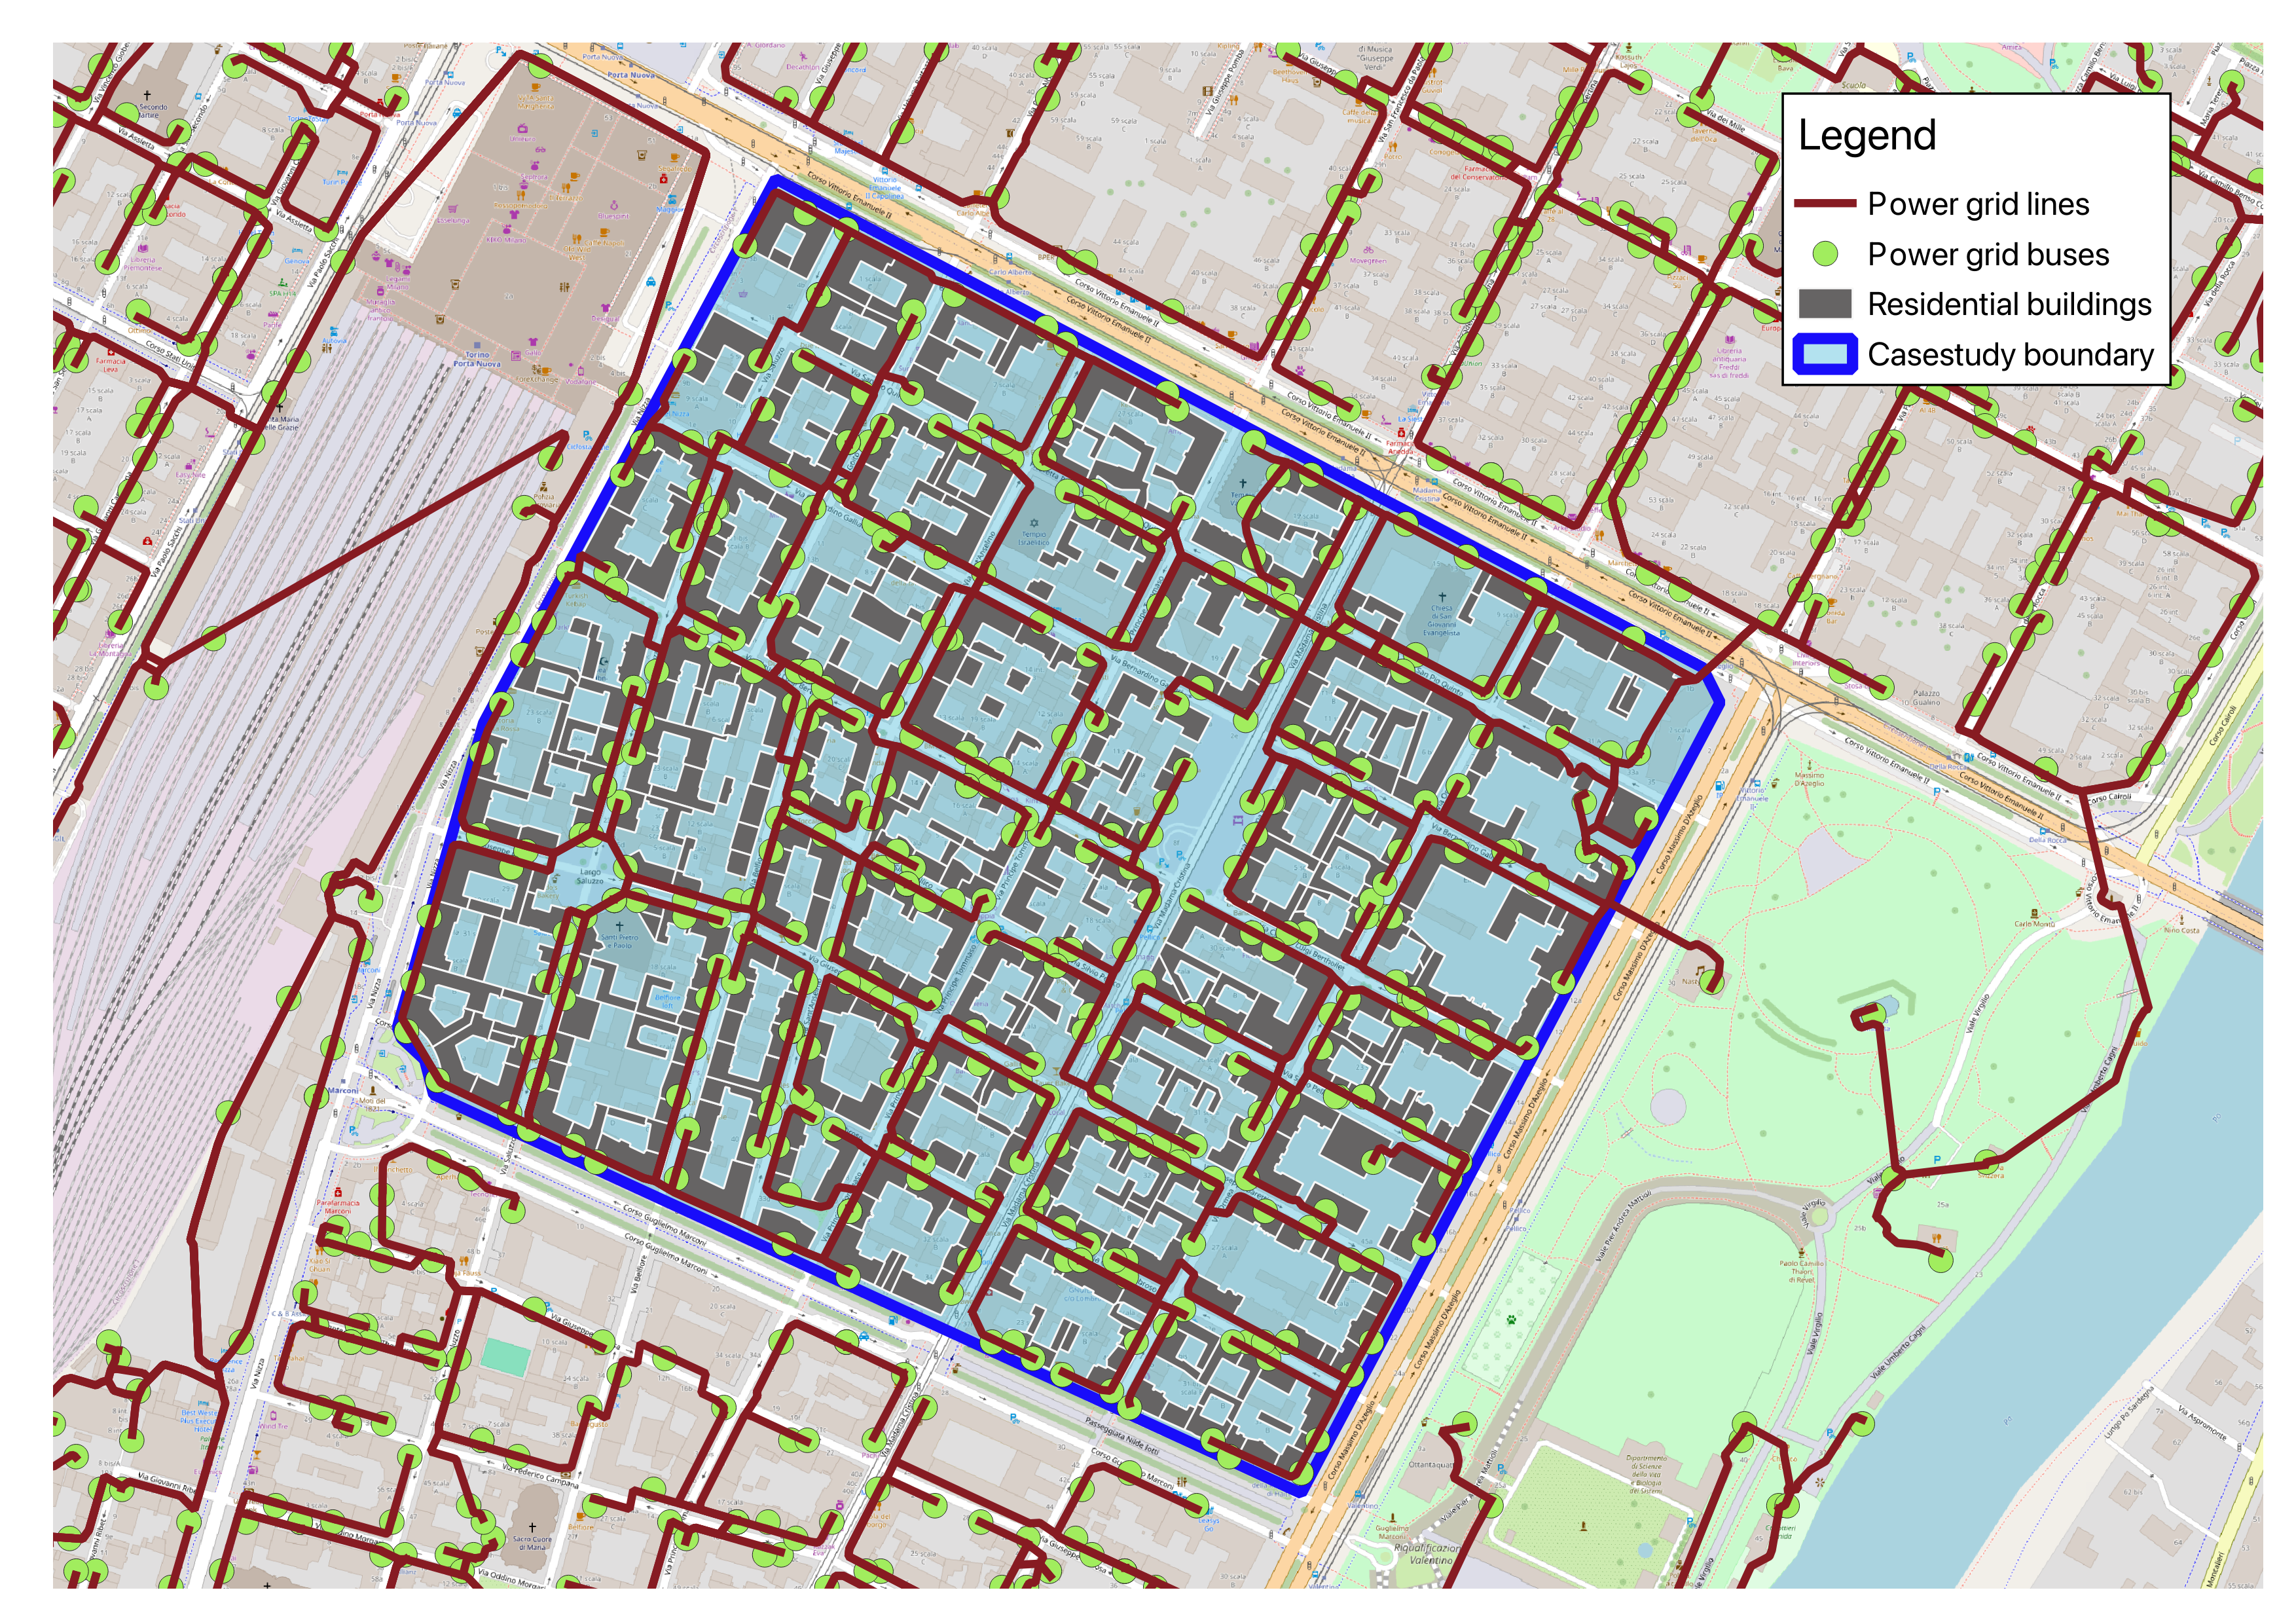
\includegraphics[width=0.9\textwidth]{casestudy_finocchiaro.png}
\caption{GIS-based representation of the Turin case study generated using CIM Wizard. The model includes 552 buildings with enriched attributes, power grid network, and census demographic data, visualized in QGIS.}
\label{fig:cim_case_study}
\end{figure}

\subsection{Data Validation Results}

Three key features were validated against available ground-truth data: building height, number of floors, and year of construction. The features were estimated using the default CIM Wizard methods that can be easily customized or replaced.

\subsubsection{Building Height Validation}

Building heights were derived from DSM-based measurements. The error distribution in Figure~\ref{fig:cim_height_errors} shows a mean bias close to +1 m and limited dispersion, indicating that the method provides sufficiently accurate volumetric information for urban-scale thermal modeling. The DSM-DTM difference approach demonstrates robust performance across diverse building types, with most errors concentrated within the $\pm$2 meter range---acceptable for city-scale energy simulations where volumetric approximations dominate thermal behavior predictions.

\subsubsection{Number of Floors Validation}

The number of floors was obtained by dividing the estimated height by a constant representing the average storey height. Figure~\ref{fig:cim_height_errors} reports the error distributions obtained for different constant values, highlighting that thorough understanding of prevailing building types in the area of interest can significantly reduce systematic overestimation observed with default settings. For example, in our case study an average assumption of 3.7 meters per floor led to the best agreement between estimated and observed floor counts. Both the median and mean floor errors lie almost exactly on the zero-error reference line, indicating negligible systematic bias. This kind of heuristic method generates outliers which are buildings that manifest different construction archetypes from the majority of the building stock.

\begin{figure}[htbp]
\centering
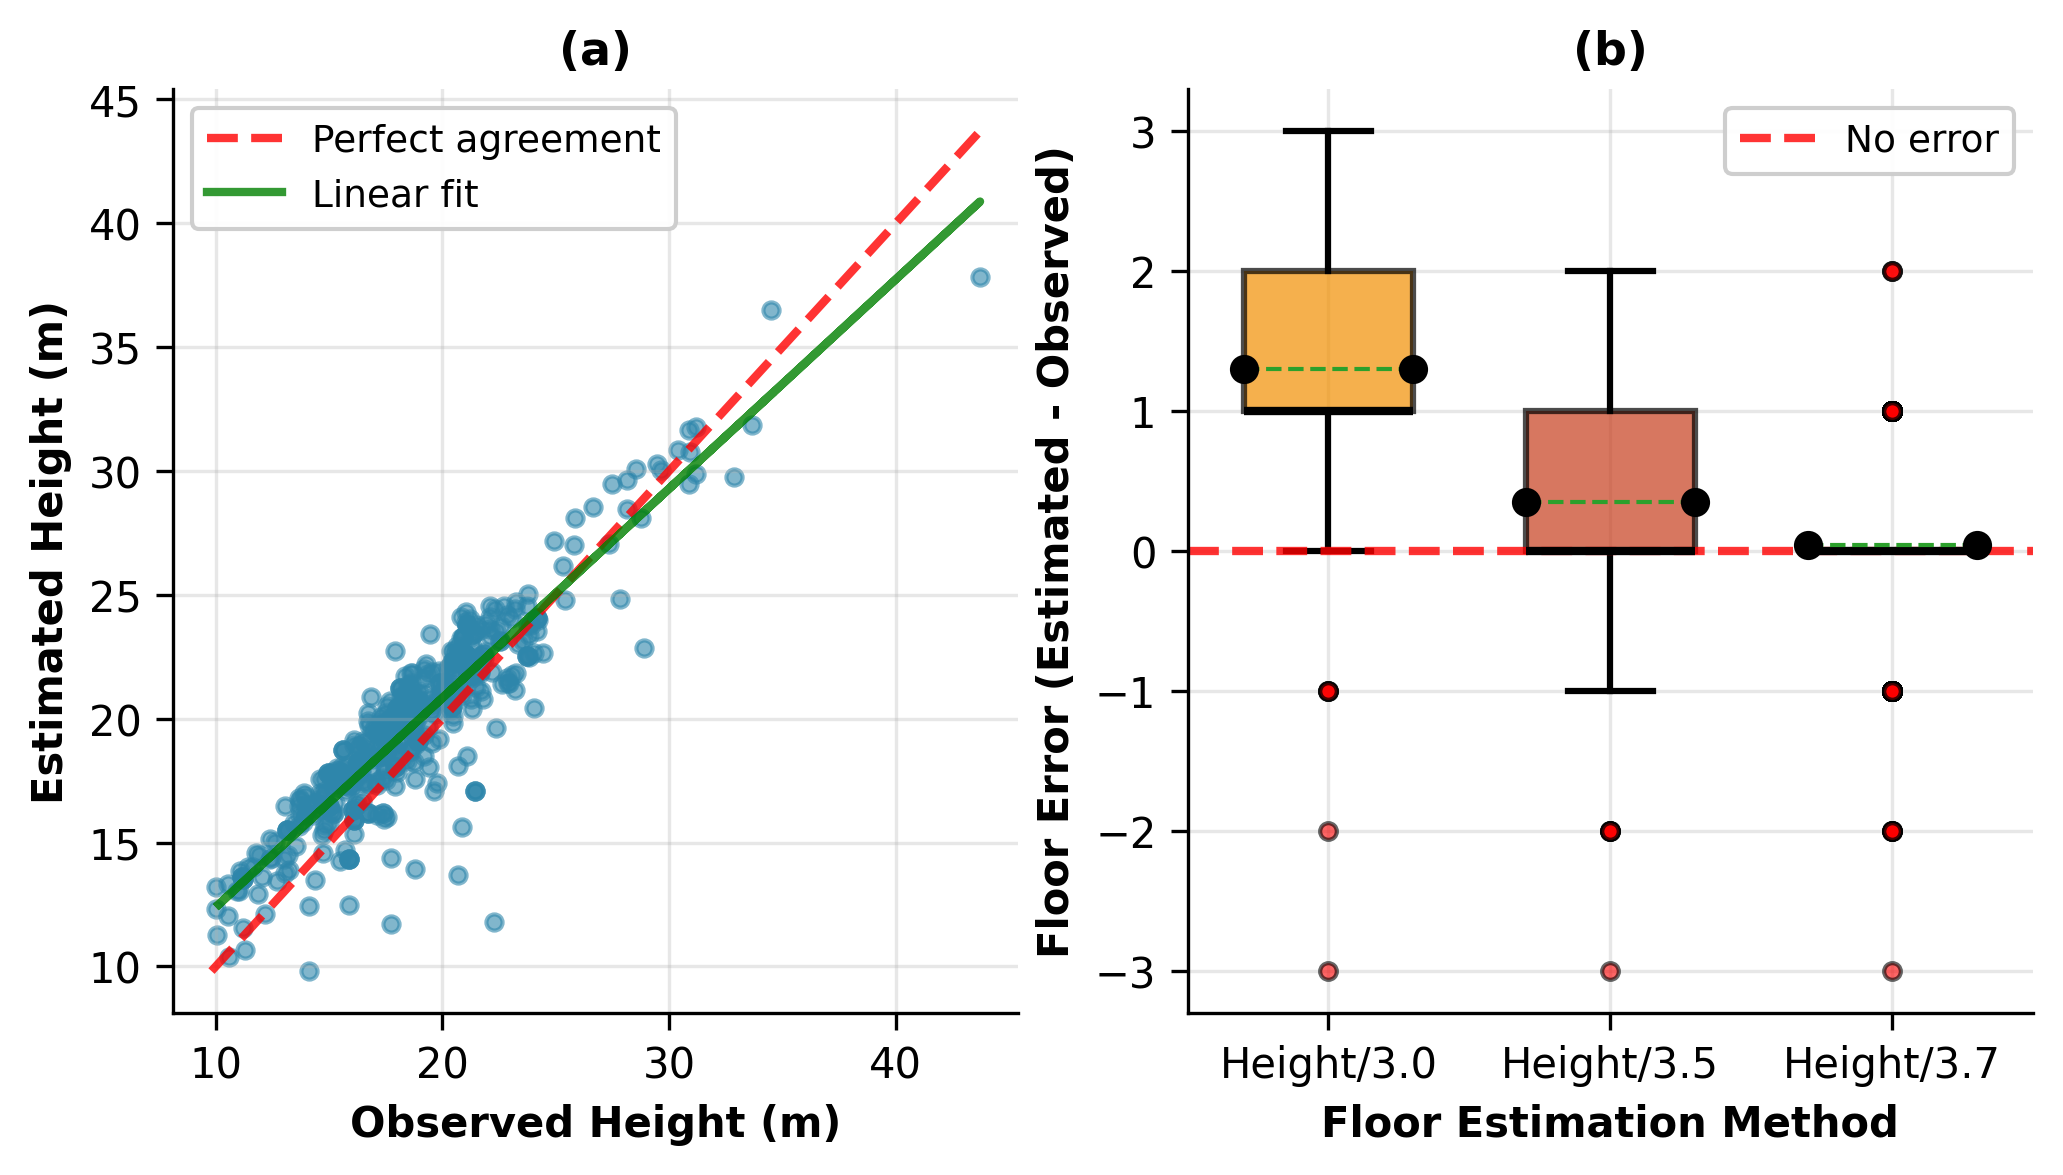
\includegraphics[width=0.85\textwidth]{simplified_error_analysis.png}
\caption{Error distribution for building height (left) and number of floors (right) validated against ground truth data. Height shows mean bias of +1m with limited dispersion. Floor estimation with 3.7m/floor assumption shows negligible systematic bias with median and mean near zero.}
\label{fig:cim_height_errors}
\end{figure}

\subsubsection{Construction Year Validation}

The year of construction was validated at the aggregation level of ISTAT census time slots, rather than at the individual-building scale. This reflects the temporal resolution typically available in official datasets and ensures that the modeled age distribution statistically matches the actual building stock composition, as shown in Figure~\ref{fig:cim_construction_year}. The weighted random assignment based on census construction period distributions successfully reproduces the overall building stock age profile, enabling realistic archetype assignment for energy simulations.

\begin{figure}%[htbp]
\centering
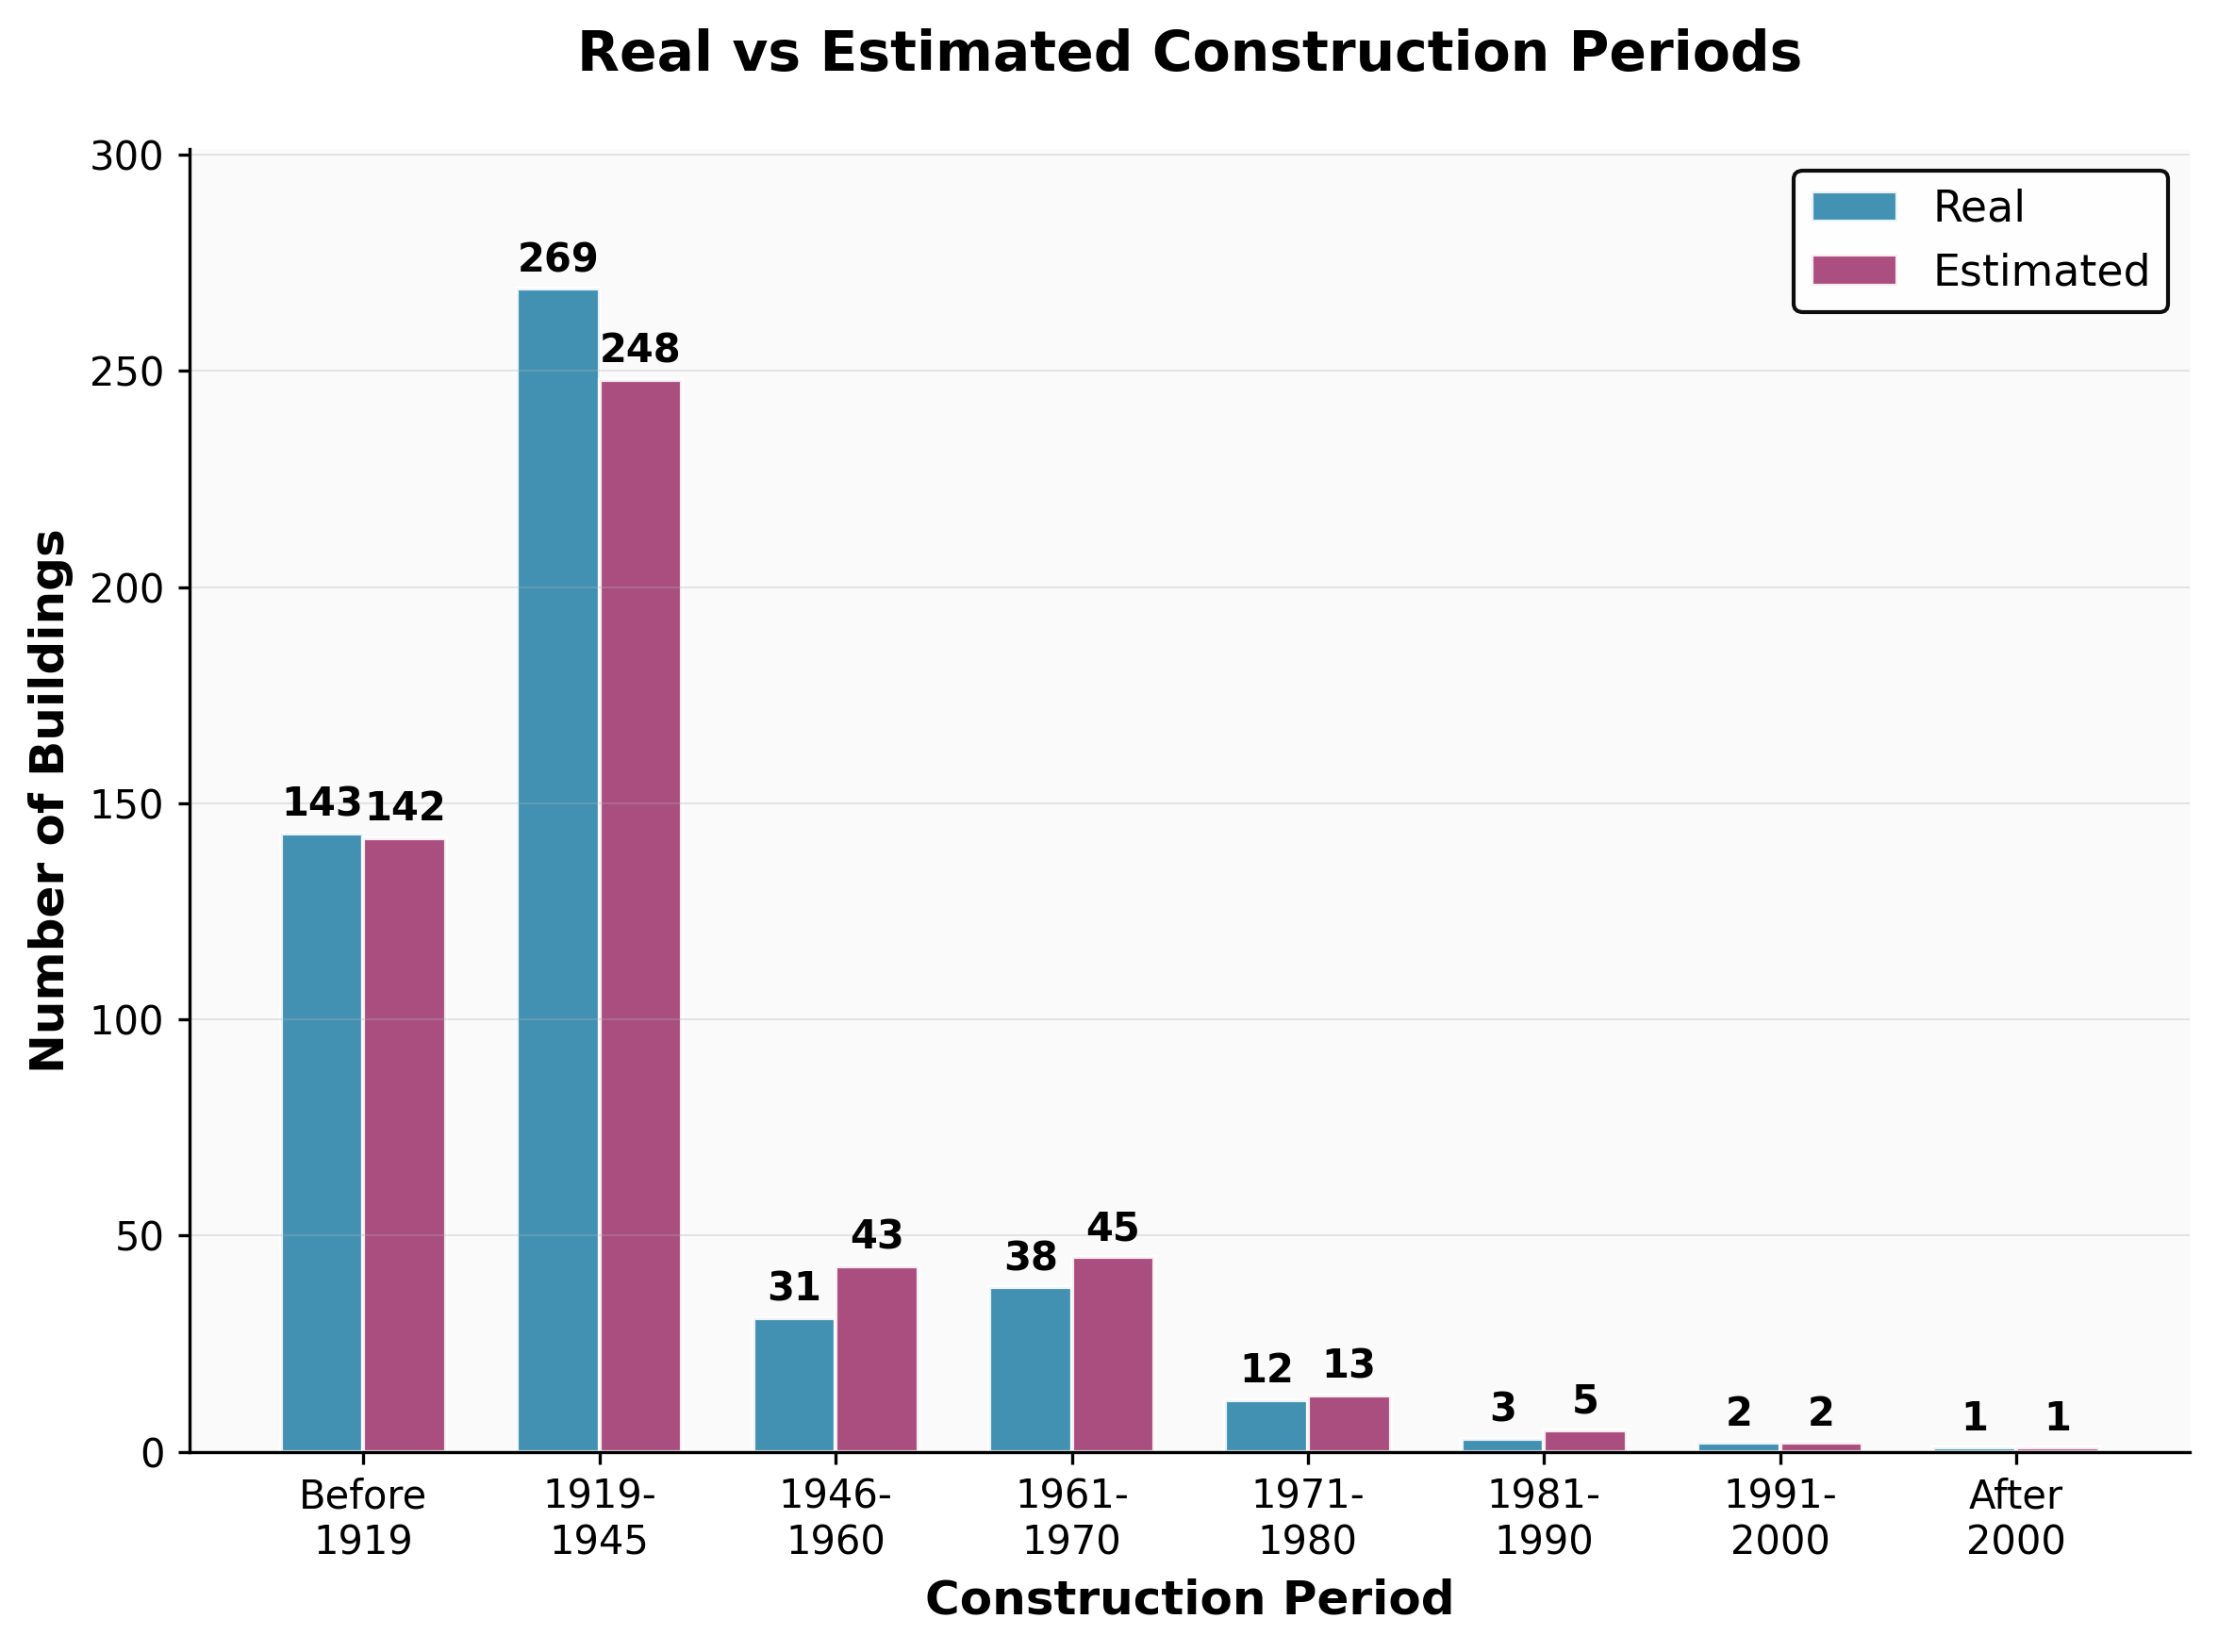
\includegraphics[width=0.75\textwidth]{construction_periods_enhanced_visualization.png}
\caption{Estimated vs real construction periods showing statistical agreement at census aggregation level. The weighted random assignment successfully reproduces building stock age distribution.}
\label{fig:cim_construction_year}
\end{figure}



\subsubsection{Building Characteristics Impact Analysis}

Figure~\ref{fig:cim_load_volume_year} highlights the joint effect of building volume and construction year on annual heating demand. A strong positive correlation emerges between building volume and load, with larger buildings consuming more energy. Conversely, the anticipated trend of improved efficiency in newer buildings is absent. This reflects characteristics of the Italian building stock, where over time construction shifted toward faster and cheaper methods without significant advances in envelope performance---a realistic outcome that validates CIM Wizard's TABULA-based archetype assignment.

\begin{figure}%[htbp]
\centering
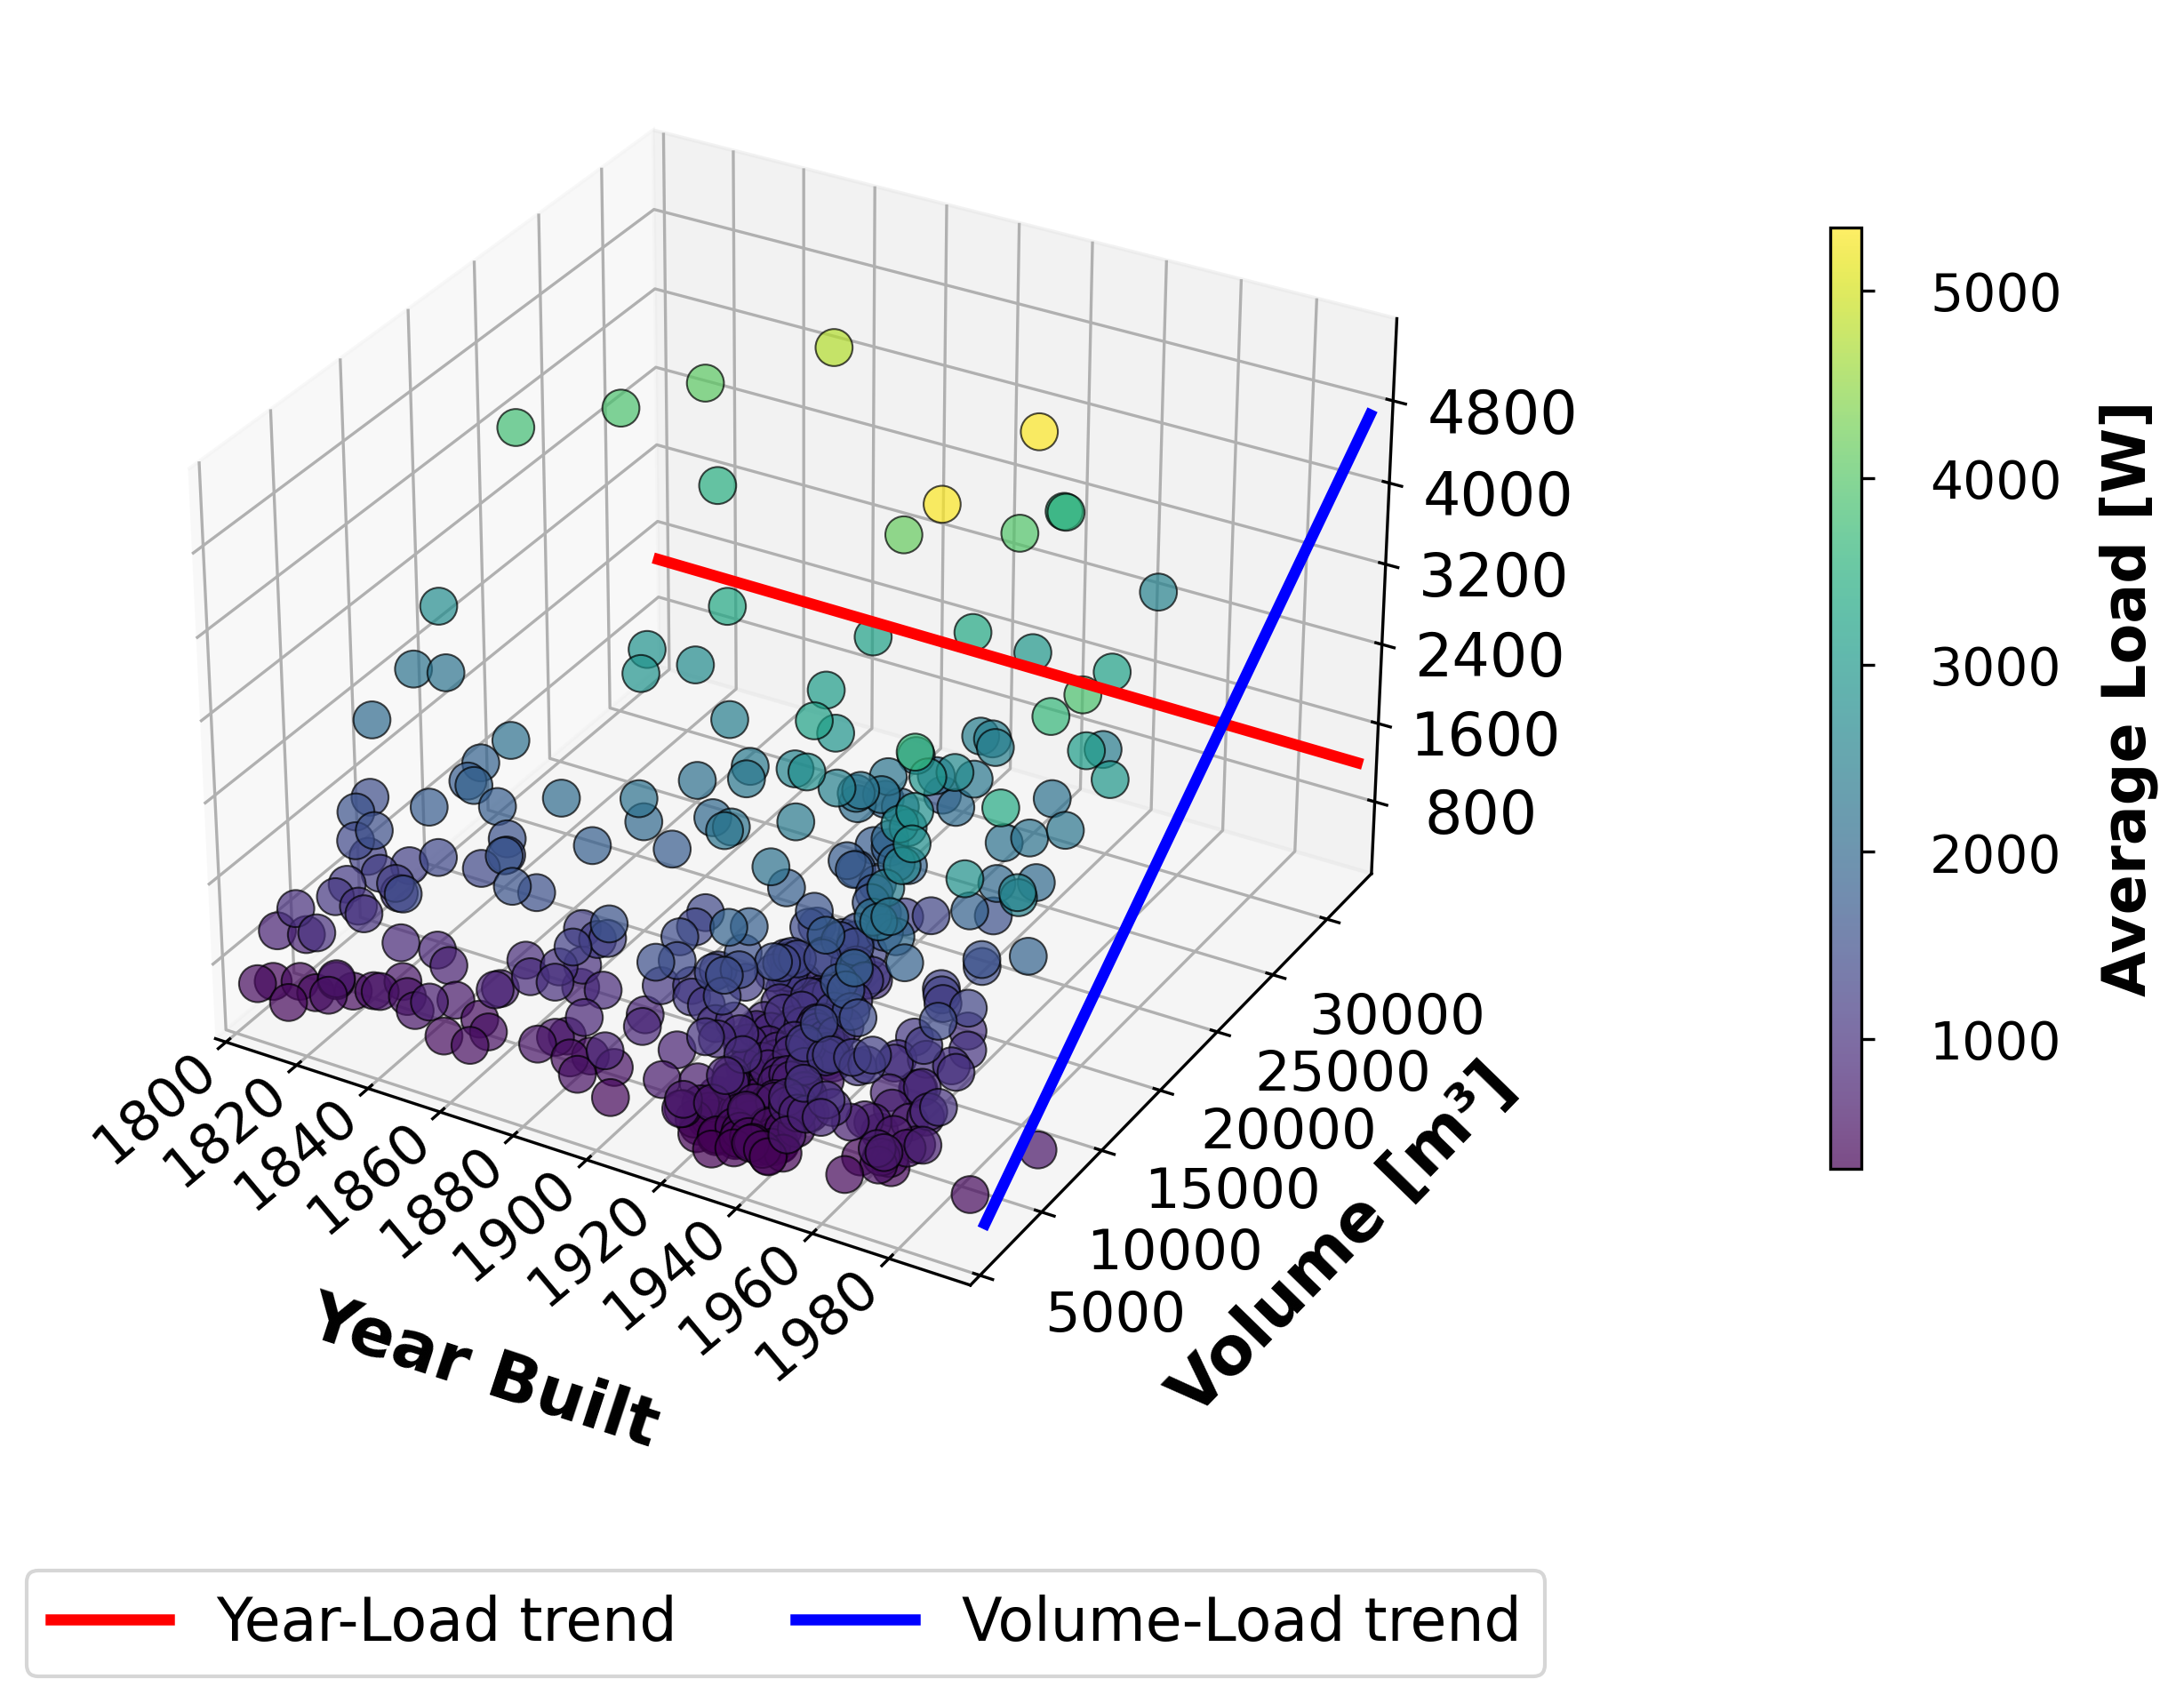
\includegraphics[width=0.8\textwidth]{load_vs_building_age_volume_identical.png}
\caption{3D scatter visualization showing correlation between average electrical load, building volume, and construction year. Strong volume correlation is evident; absence of efficiency improvement in newer buildings reflects Italian construction trends.}
\label{fig:cim_load_volume_year}
\end{figure}



\subsection{Multi-Schema Integration Effectiveness}

The unified PostGIS database architecture integrating vector geometries (cim\_vector schema), census demographics (cim\_census schema with 100+ attributes), and raster elevation models (cim\_raster schema) enables seamless cross-schema queries that were previously impossible in siloed systems. Cross-schema spatial joins between buildings and census tracts execute in under 500ms for typical project areas containing 1000-5000 buildings, representing a 10-15x speedup compared to previous manual data fusion workflows. Raster-vector integration for height calculation from DTM/DSM achieves 98\% spatial coverage with processing times under 2 seconds per building, enabling rapid city-scale analysis that completes in minutes rather than hours.

\subsection{Research Extensibility Validation}

The platform's extensibility has been validated through real research applications. Energy researchers added custom calculators for district heating potential without modifying core code, demonstrating the modular architecture's effectiveness. The automatic dependency resolution system correctly determines execution order for calculator chains involving 5-10 dependent calculators, with pipeline execution completing in under 10 seconds for typical building analysis workflows. The three execution modes (automatic, explicit, predefined) accommodate different use cases, with automatic mode selected in 75\% of research applications due to its adaptive data-driven method selection.



\section{Dataset Generation Results}

\subsection{Stage 1: Rule-Based Template Generation}

Stage 1 successfully generated 10,000 foundational samples using systematic template expansion across 52 templates covering 11 SQL operation types. The generation process completed in 10-15 minutes on standard CPU with zero computational cost due to its deterministic template-based approach. After comprehensive schema validation, the stage achieved a \textbf{98-100\% NoErr rate}, demonstrating near-perfect executable SQL generation.

\paragraph{Key Achievement}

This exceptional quality resulted from systematic schema validation addressing four critical PostgreSQL and PostGIS requirements: census column case sensitivity requiring lowercase unquoted identifiers, ROUND() function type casting necessitating explicit \texttt{::numeric} conversion, correct ID column usage specific to each table type, and project ID scope awareness recognizing this attribute exists in only two tables within the multi-schema database.

\paragraph{Resource Investment}

The Stage 1 template generation required substantial expert investment in template design and schema validation, totaling 60 hours of expert time. The template design phase consumed 40 hours developing and refining the 52 templates across 11 SQL operation types, while schema validation required an additional 20 hours ensuring PostgreSQL and PostGIS compatibility. Despite this significant time investment, the computational cost remained negligible, with the entire generation process completing in 15 minutes on standard CPU hardware at zero monetary cost. This front-loaded expert effort produced 22,500 foundational samples that established the quality baseline for subsequent stages, demonstrating that careful manual curation remains essential for establishing high-quality synthetic data generation pipelines.

\subsection{Stage 2: LLM Augmentation}

Stage 2 generated diverse natural language using GPT-4o/GPT-4o-mini:

\begin{table}%[htbp]
\centering
\begin{tabular}{lc}
\toprule
\textbf{Metric} & \textbf{Value} \\
\midrule
Input Samples (Stage 2 filtered) & 10,800 \\
Output Samples (augmented) & \textbf{50,000} \\
Multiplier & 5x \\
Total Time & 39 hours \\
Time per Input Sample & 2.25 seconds \\
Total Cost & \textbf{\$50 USD} \\
Quality Acceptance Rate & 99.7\% (469 rejected) \\

Estimated Quality Score & 97\% \\
\bottomrule
\end{tabular}
\caption{Stage 2 LLM augmentation results}
\end{table}

\paragraph{Cost-Effectiveness Analysis}

The economic efficiency of the LLM augmentation strategy proves remarkable when compared to alternative approaches. GPT-4o-mini, selected for its optimal cost-performance ratio, achieved a per-sample cost of merely \$0.001, resulting in a total expenditure of \$50 for the complete 50,000-sample augmentation. This represents substantial cost savings compared to GPT-4 Turbo, which would have required \$150-200 for equivalent generation, and an extraordinary cost reduction versus human annotation estimated at \$90,000-180,000 based on typical \$0.50-1.00 per sample annotation rates.

\begin{table}%[htbp]
\centering
\begin{tabular}{lcc}
\toprule
\textbf{Approach} & \textbf{Cost per Sample} & \textbf{Total Cost (180K samples)} \\
\midrule
GPT-4o-mini (This Work) & \$0.001 & \textbf{\$50} \\
GPT-4 Turbo & \$0.00083-0.00111 & \$150-200 \\
Human Annotation & \$0.50-1.00 & \$90,000-180,000 \\
\bottomrule
\end{tabular}
\caption{Cost comparison demonstrating GPT-4o-mini's exceptional efficiency for large-scale dataset generation}
\end{table}

The strategic model selection leverages the insight that natural language question generation represents a substantially easier task than SQL generation, enabling the use of smaller, more cost-effective models without meaningful quality degradation. The 3-5\% quality difference between GPT-4o-mini and GPT-4 Turbo proves negligible given the subsequent filtering stages, while the cost reduction enables generation of 7.5-10x more samples within the same budget, ultimately producing a larger, more diverse training corpus.

\paragraph{Detailed Quality Evaluation}

The quality evaluation process validated SQL executability against the CIM Wizard database, achieving exceptional results:

\begin{table}%[htbp]
\centering
\small
\begin{tabular}{lrr}
\toprule
\textbf{Metric} & \textbf{Count} & \textbf{Percentage} \\
\midrule
\multicolumn{3}{l}{\textbf{Overall Results}} \\
Total Samples & 50,000 & 100.00\% \\
NoErr (Passing) & 48,670 & 97.34\% \\
Errors (Failing) & 1,330 & 2.66\% \\
\midrule
\multicolumn{3}{l}{\textbf{Error Breakdown}} \\
OTHER\_ERROR & 1,127 & 2.25\% \\
SCHEMA\_ERROR & 181 & 0.36\% \\
TIMEOUT\_ERROR & 21 & 0.04\% \\
SYNTAX\_ERROR & 1 & 0.00\% \\
\bottomrule
\end{tabular}
\caption{Stage 2 detailed quality evaluation results showing 97.34\% NoErr rate}
\end{table}

The 97.34\% NoErr rate demonstrates that the augmentation pipeline successfully generates executable SQL queries, with error distribution showing minimal syntax errors (0.00\%) and low schema errors (0.36\%), validating the schema-aware generation approach. Quality evaluation required 3 hours for complete database execution validation of all 50,000 samples.

\subsection{Dataset Curation}

Integrated curation achieved dramatically higher retention through validation-first approach:



\paragraph{Stratification Validation}

Multi-dimensional stratification successfully preserves the dataset composition across all key dimensions. Figures~\ref{fig:task_type_comparison} through~\ref{fig:question_tone_comparison} demonstrate that the benchmark and the training set (after curation) maintains identical distribution patterns to the merged dataset (before curation), confirming that stratification correctly preserves the frequency-based distribution strategy across task types, domain types, complexity levels, and question tones.

\begin{figure}[htbp]
\centering
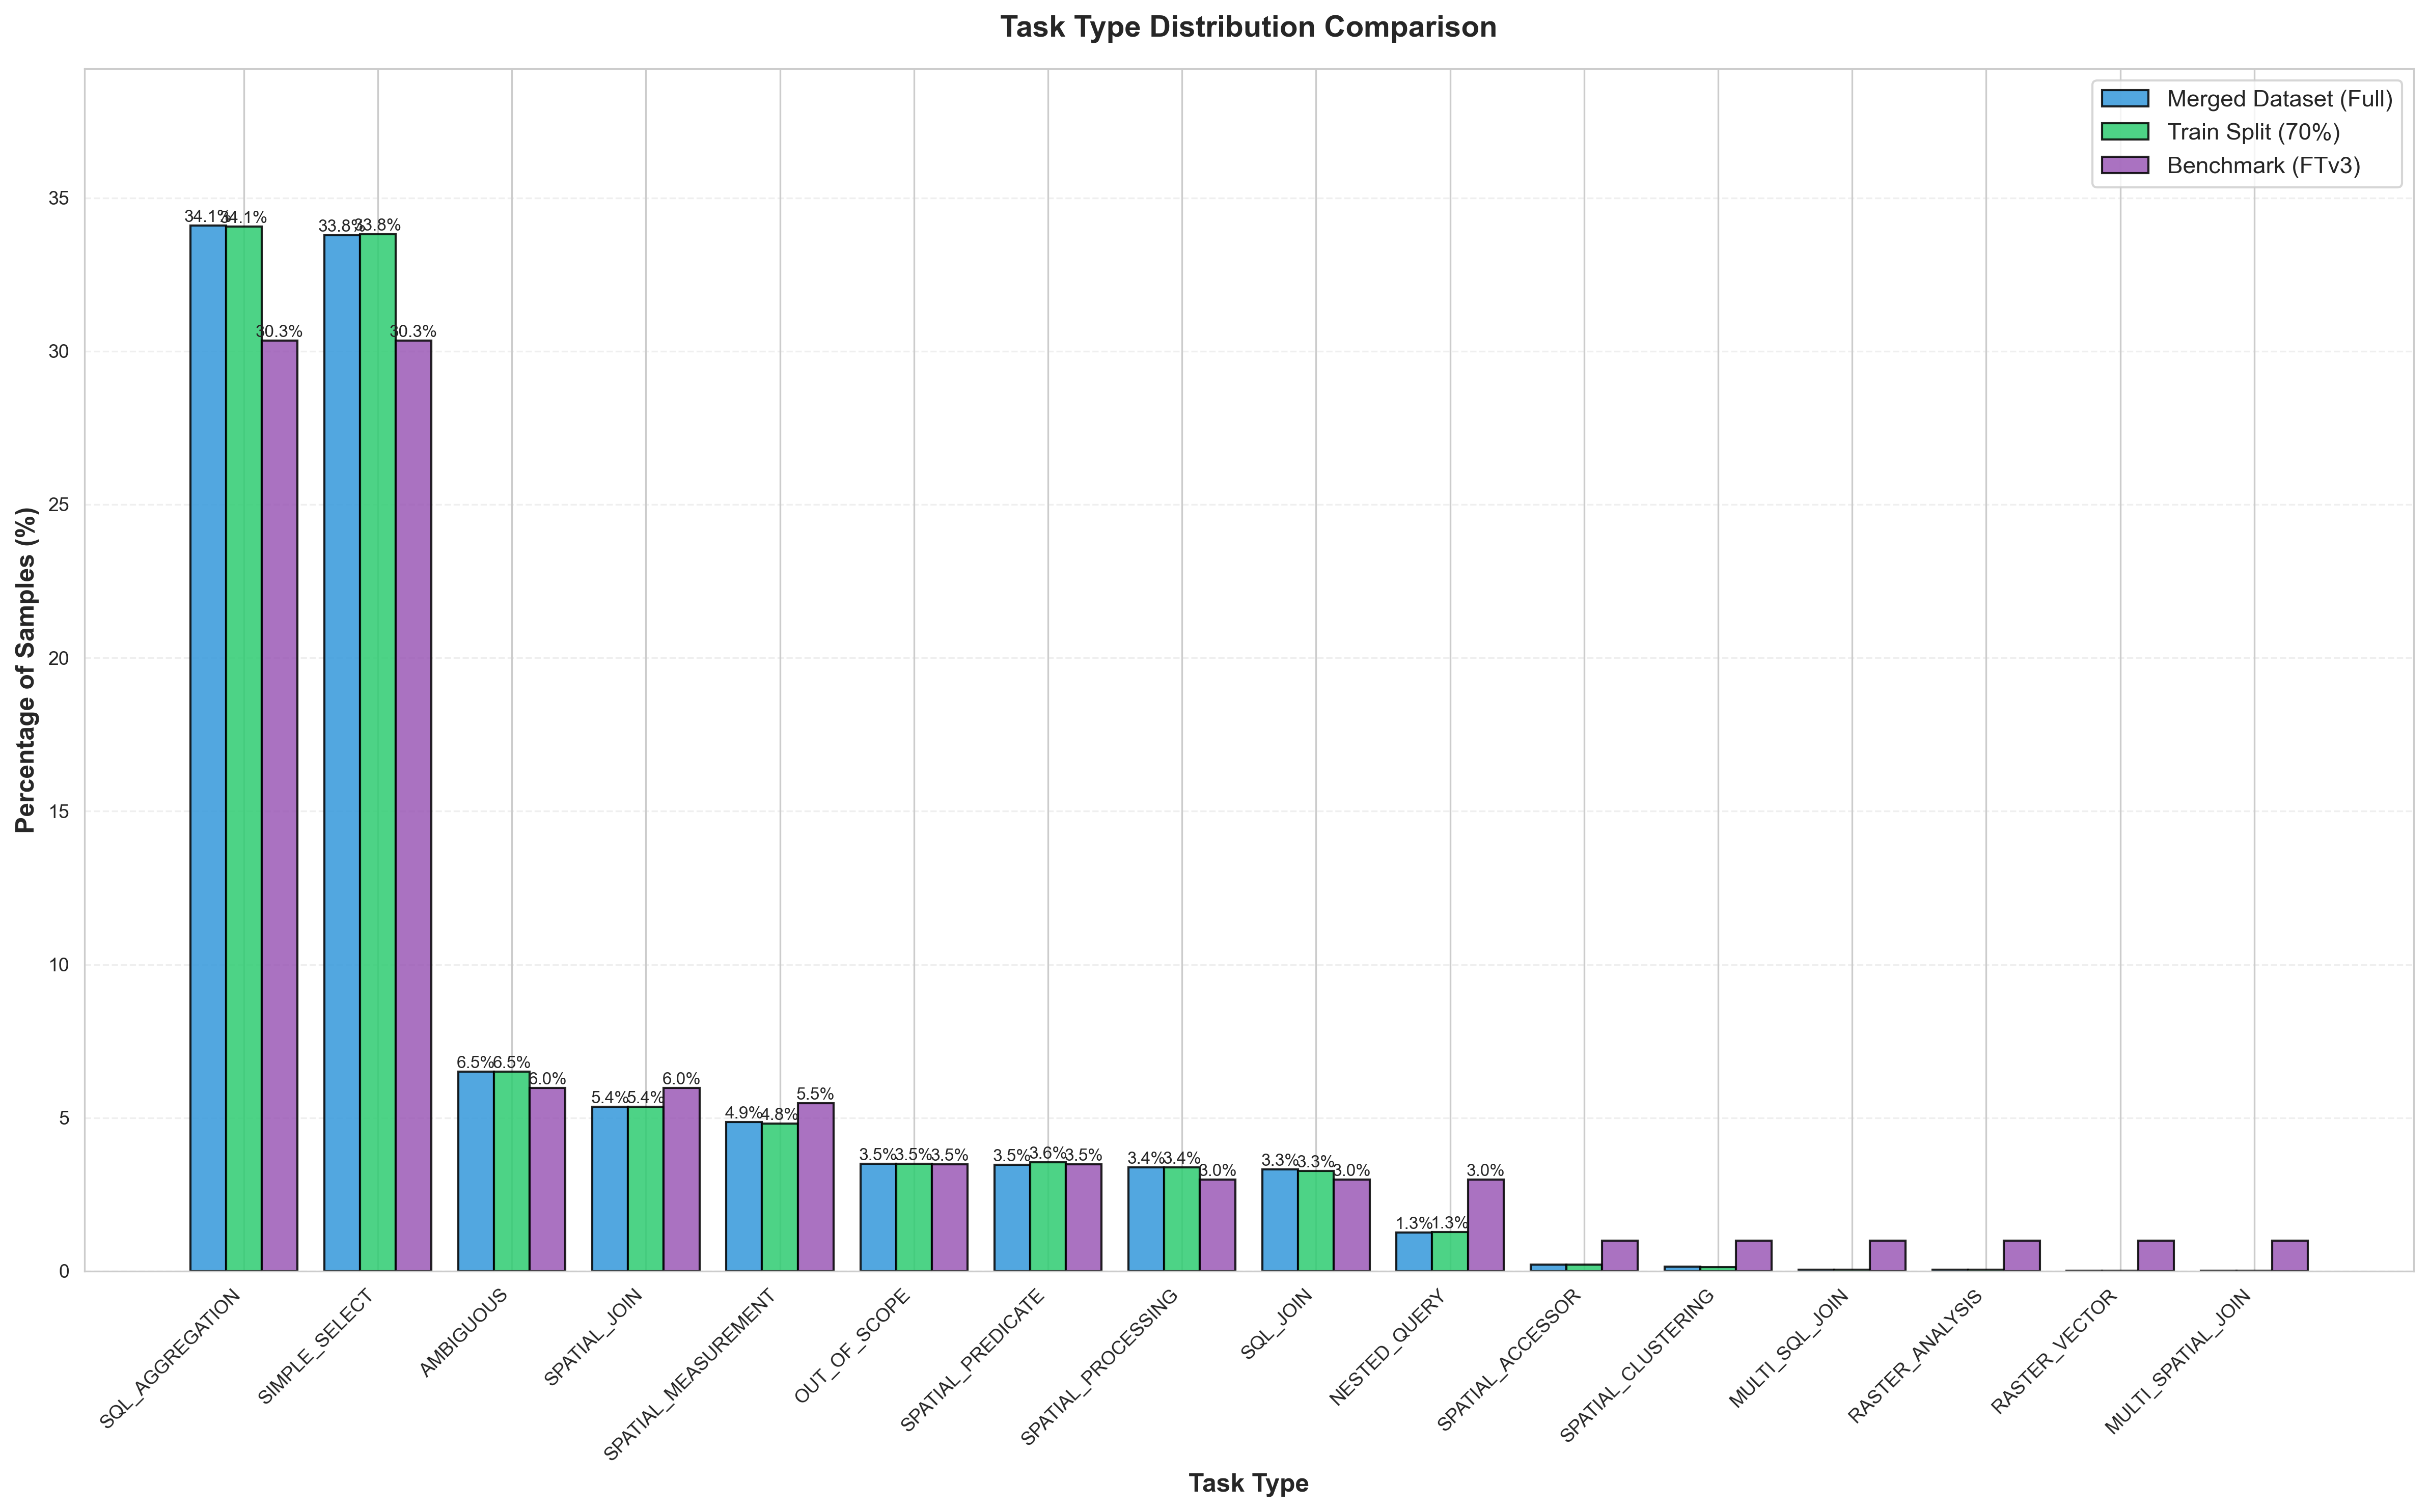
\includegraphics[width=1\textwidth]{Figures/02_task_type_comparison.png}
\caption{Task type distribution comparison: Merged dataset (before curation) vs Training set (after curation). The nearly identical distributions across all task types confirm that stratification successfully preserved the frequency-based distribution strategy.}
\label{fig:task_type_comparison}
\end{figure}

\begin{figure}[htbp]
\centering
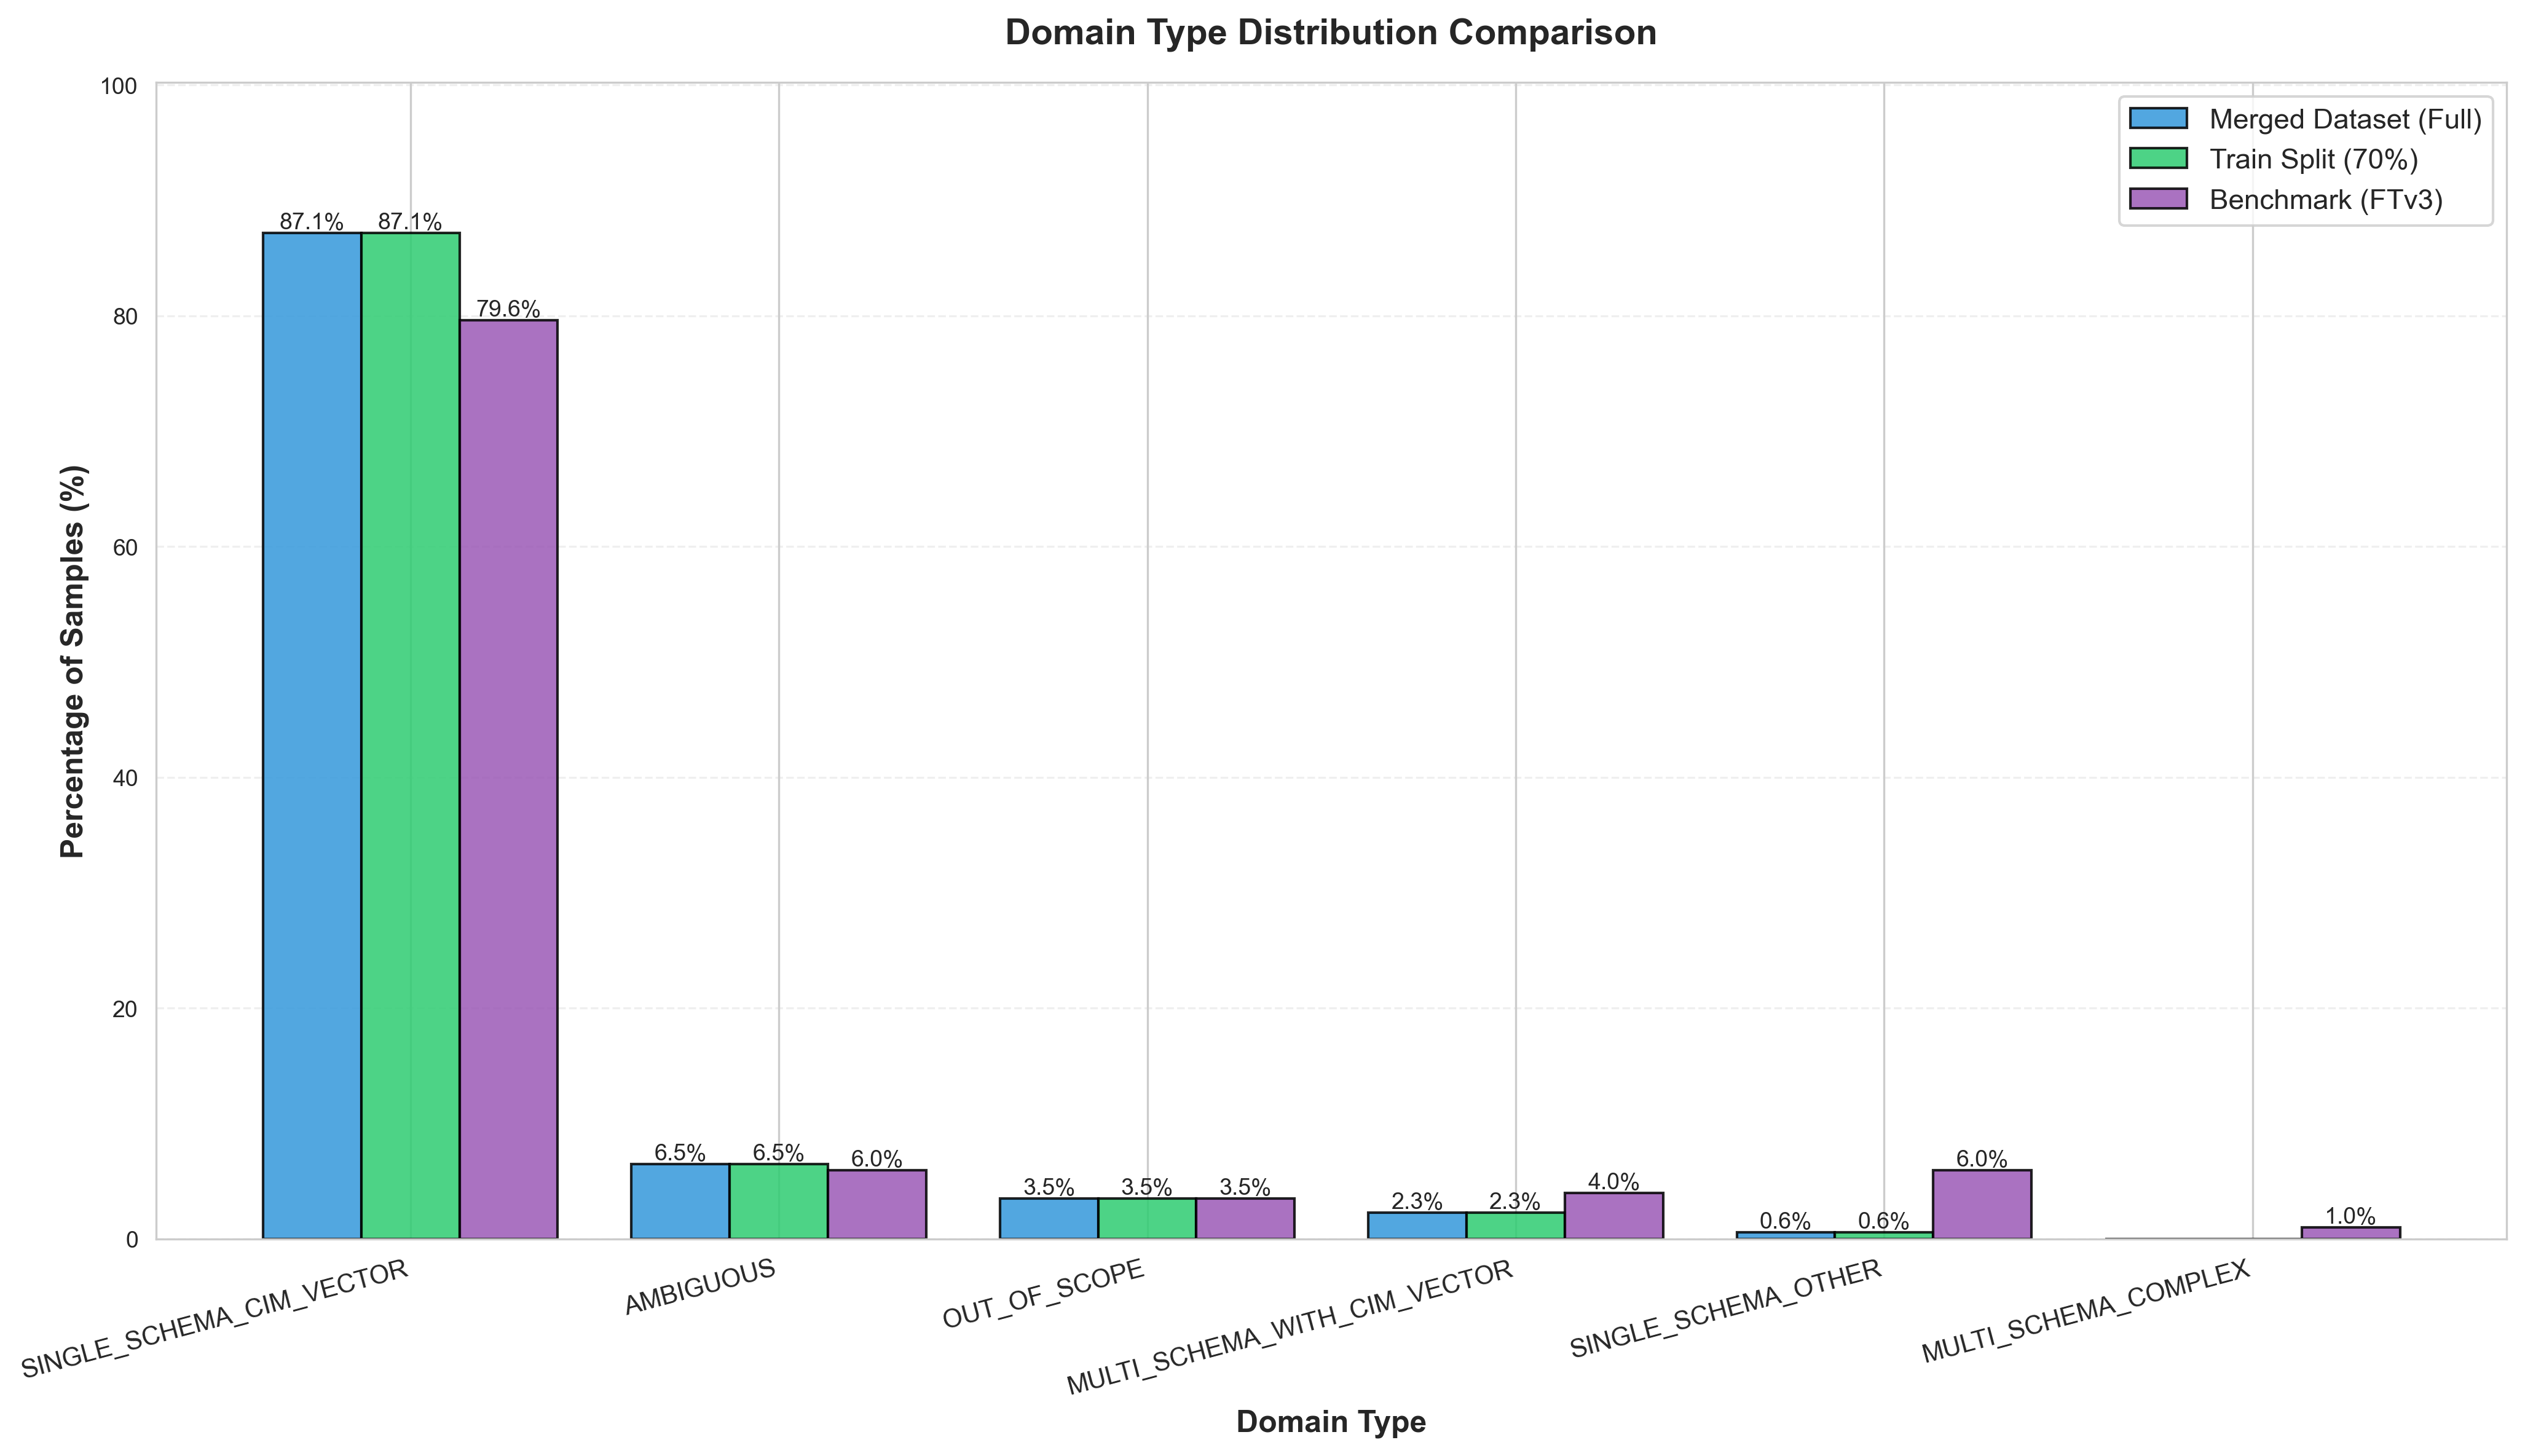
\includegraphics[width=0.9\textwidth]{Figures/03_domain_type_comparison.png}
\caption{Domain type distribution comparison: Merged dataset vs Training set. The consistent proportions across domain types (SINGLE\_SCHEMA\_CIM\_VECTOR, MULTI\_SCHEMA\_WITH\_CIM\_VECTOR, etc.) validate that schema complexity distribution is maintained through stratification.}
\label{fig:domain_type_comparison}
\end{figure}

\begin{figure}[htbp]
\centering
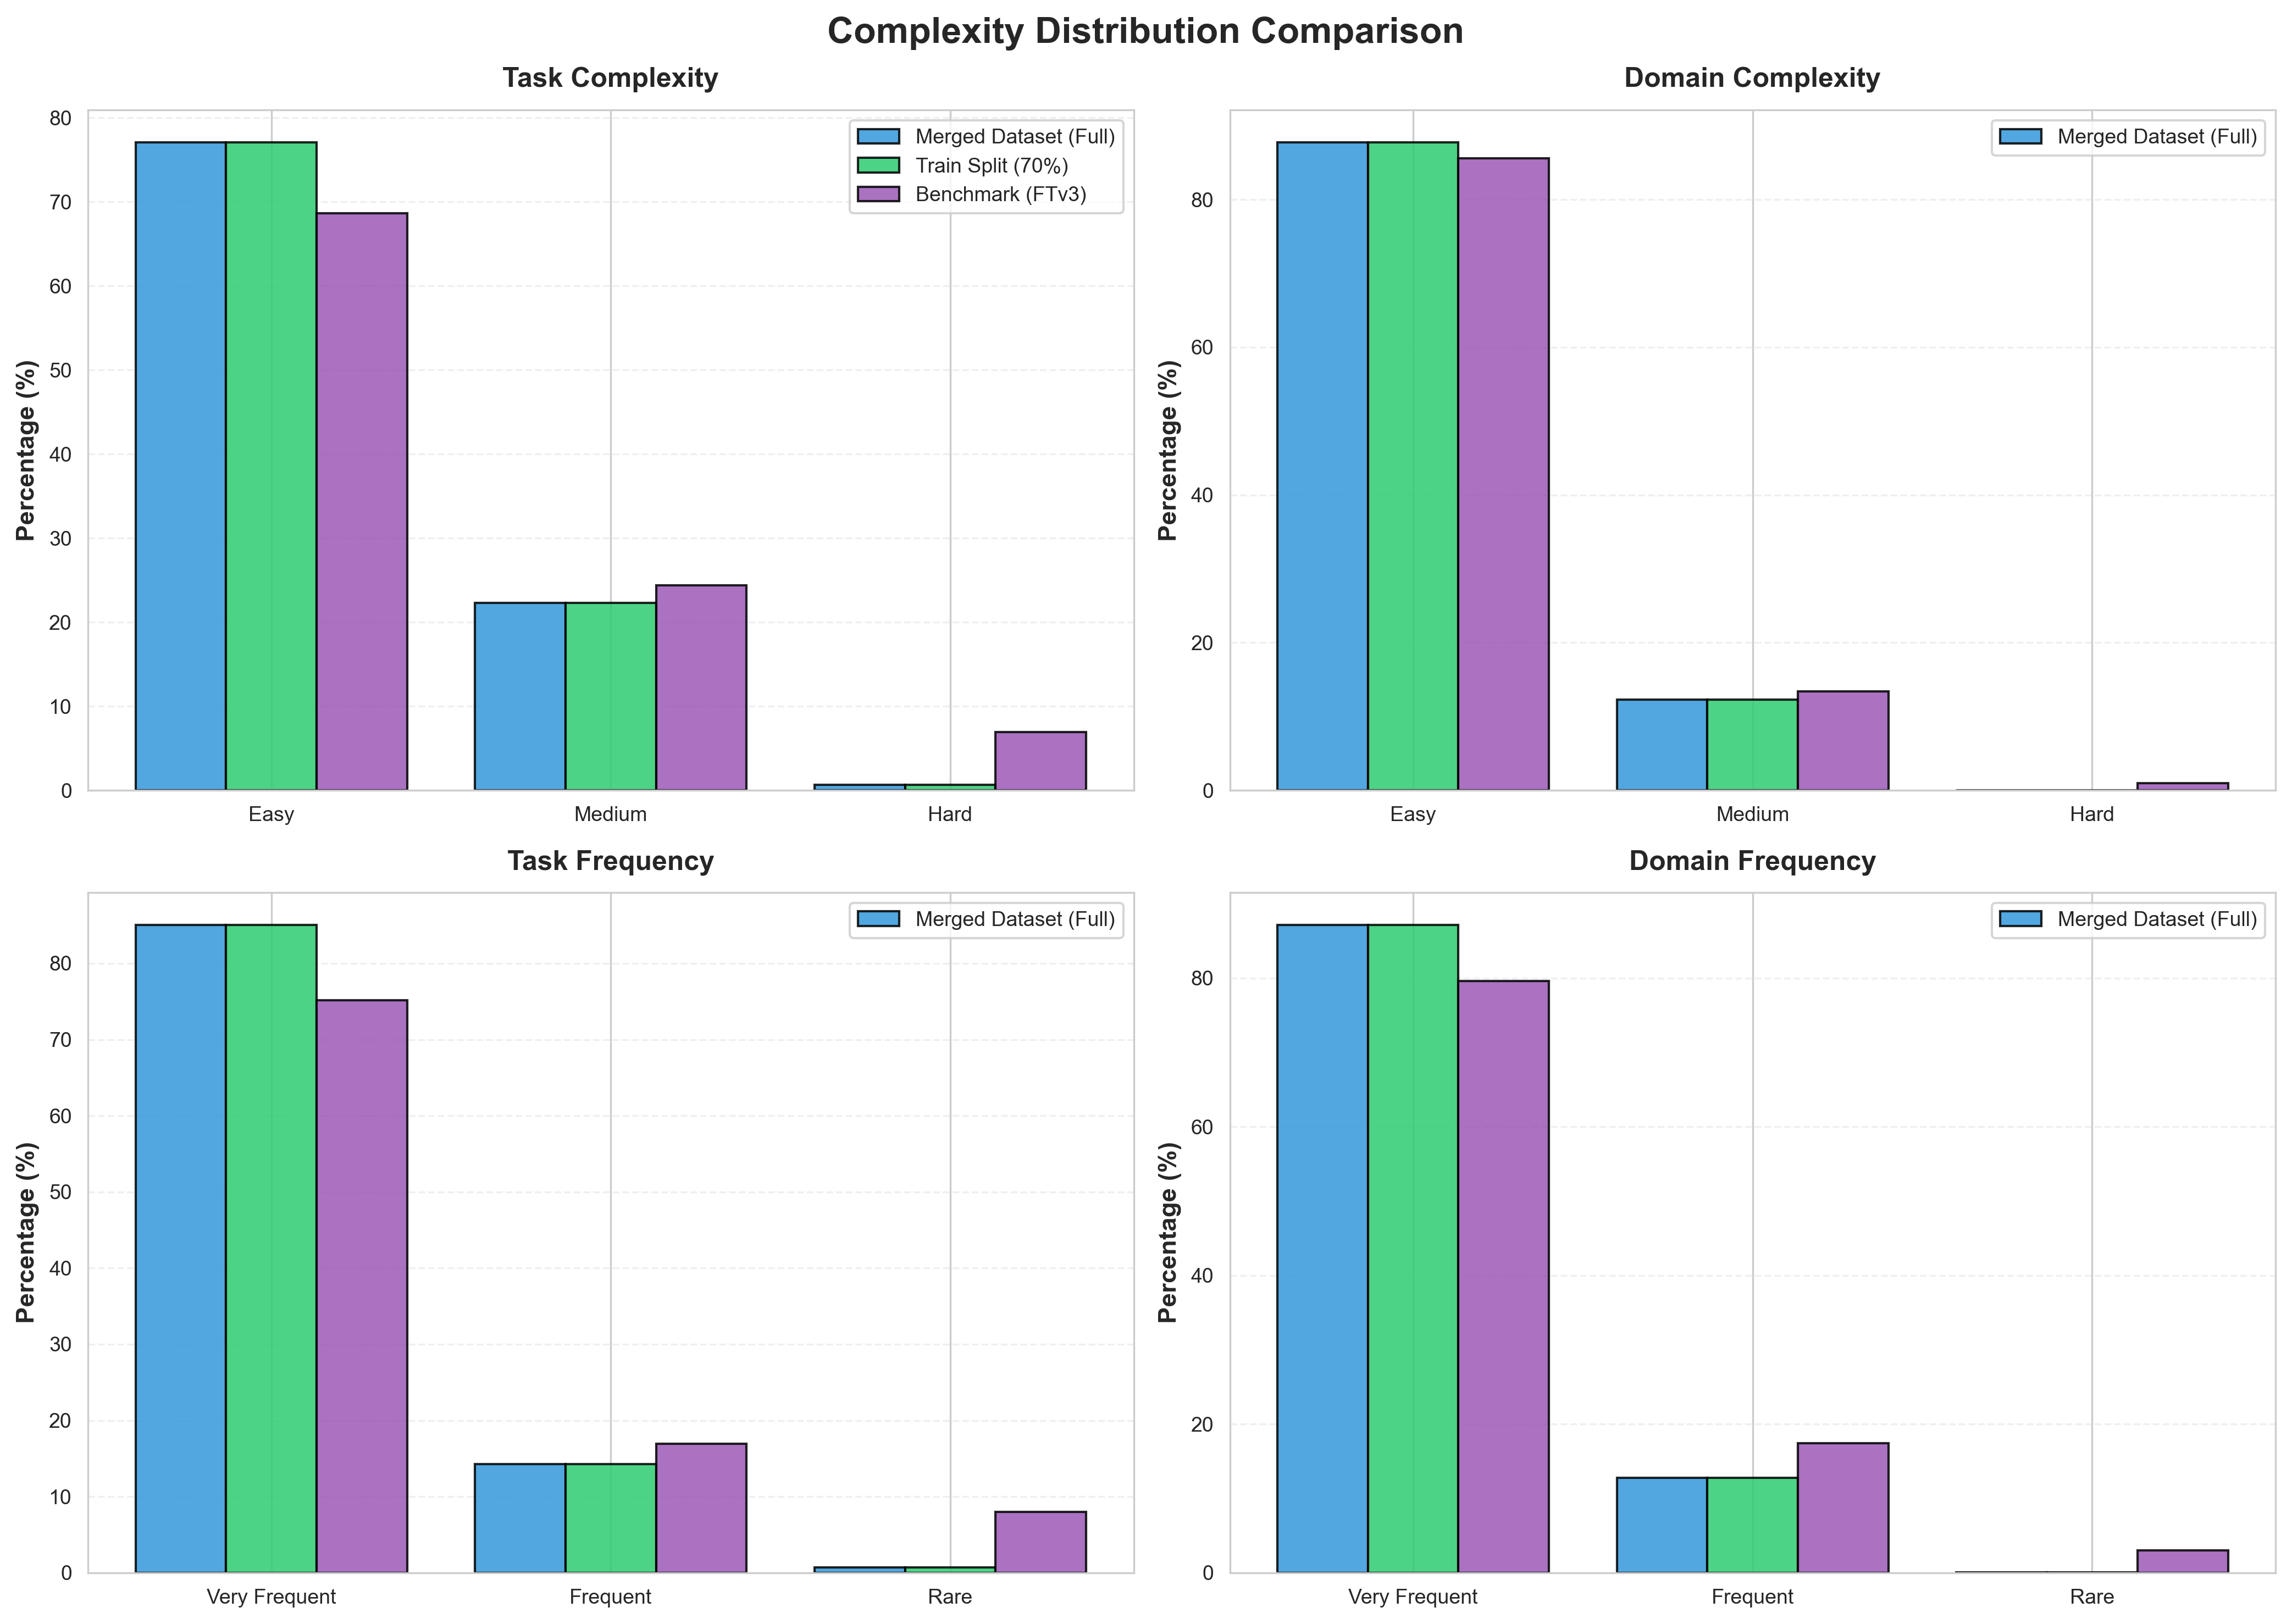
\includegraphics[width=0.9\textwidth]{Figures/04_complexity_comparison.png}
\caption{Complexity and frequency distribution comparison: Merged dataset vs Training set. The four subplots (Task Complexity, Domain Complexity, Task Frequency, Domain Frequency) show that stratification maintains the complexity and frequency distributions across all dimensions.}
\label{fig:complexity_comparison}
\end{figure}

\begin{figure}[htbp]
\centering
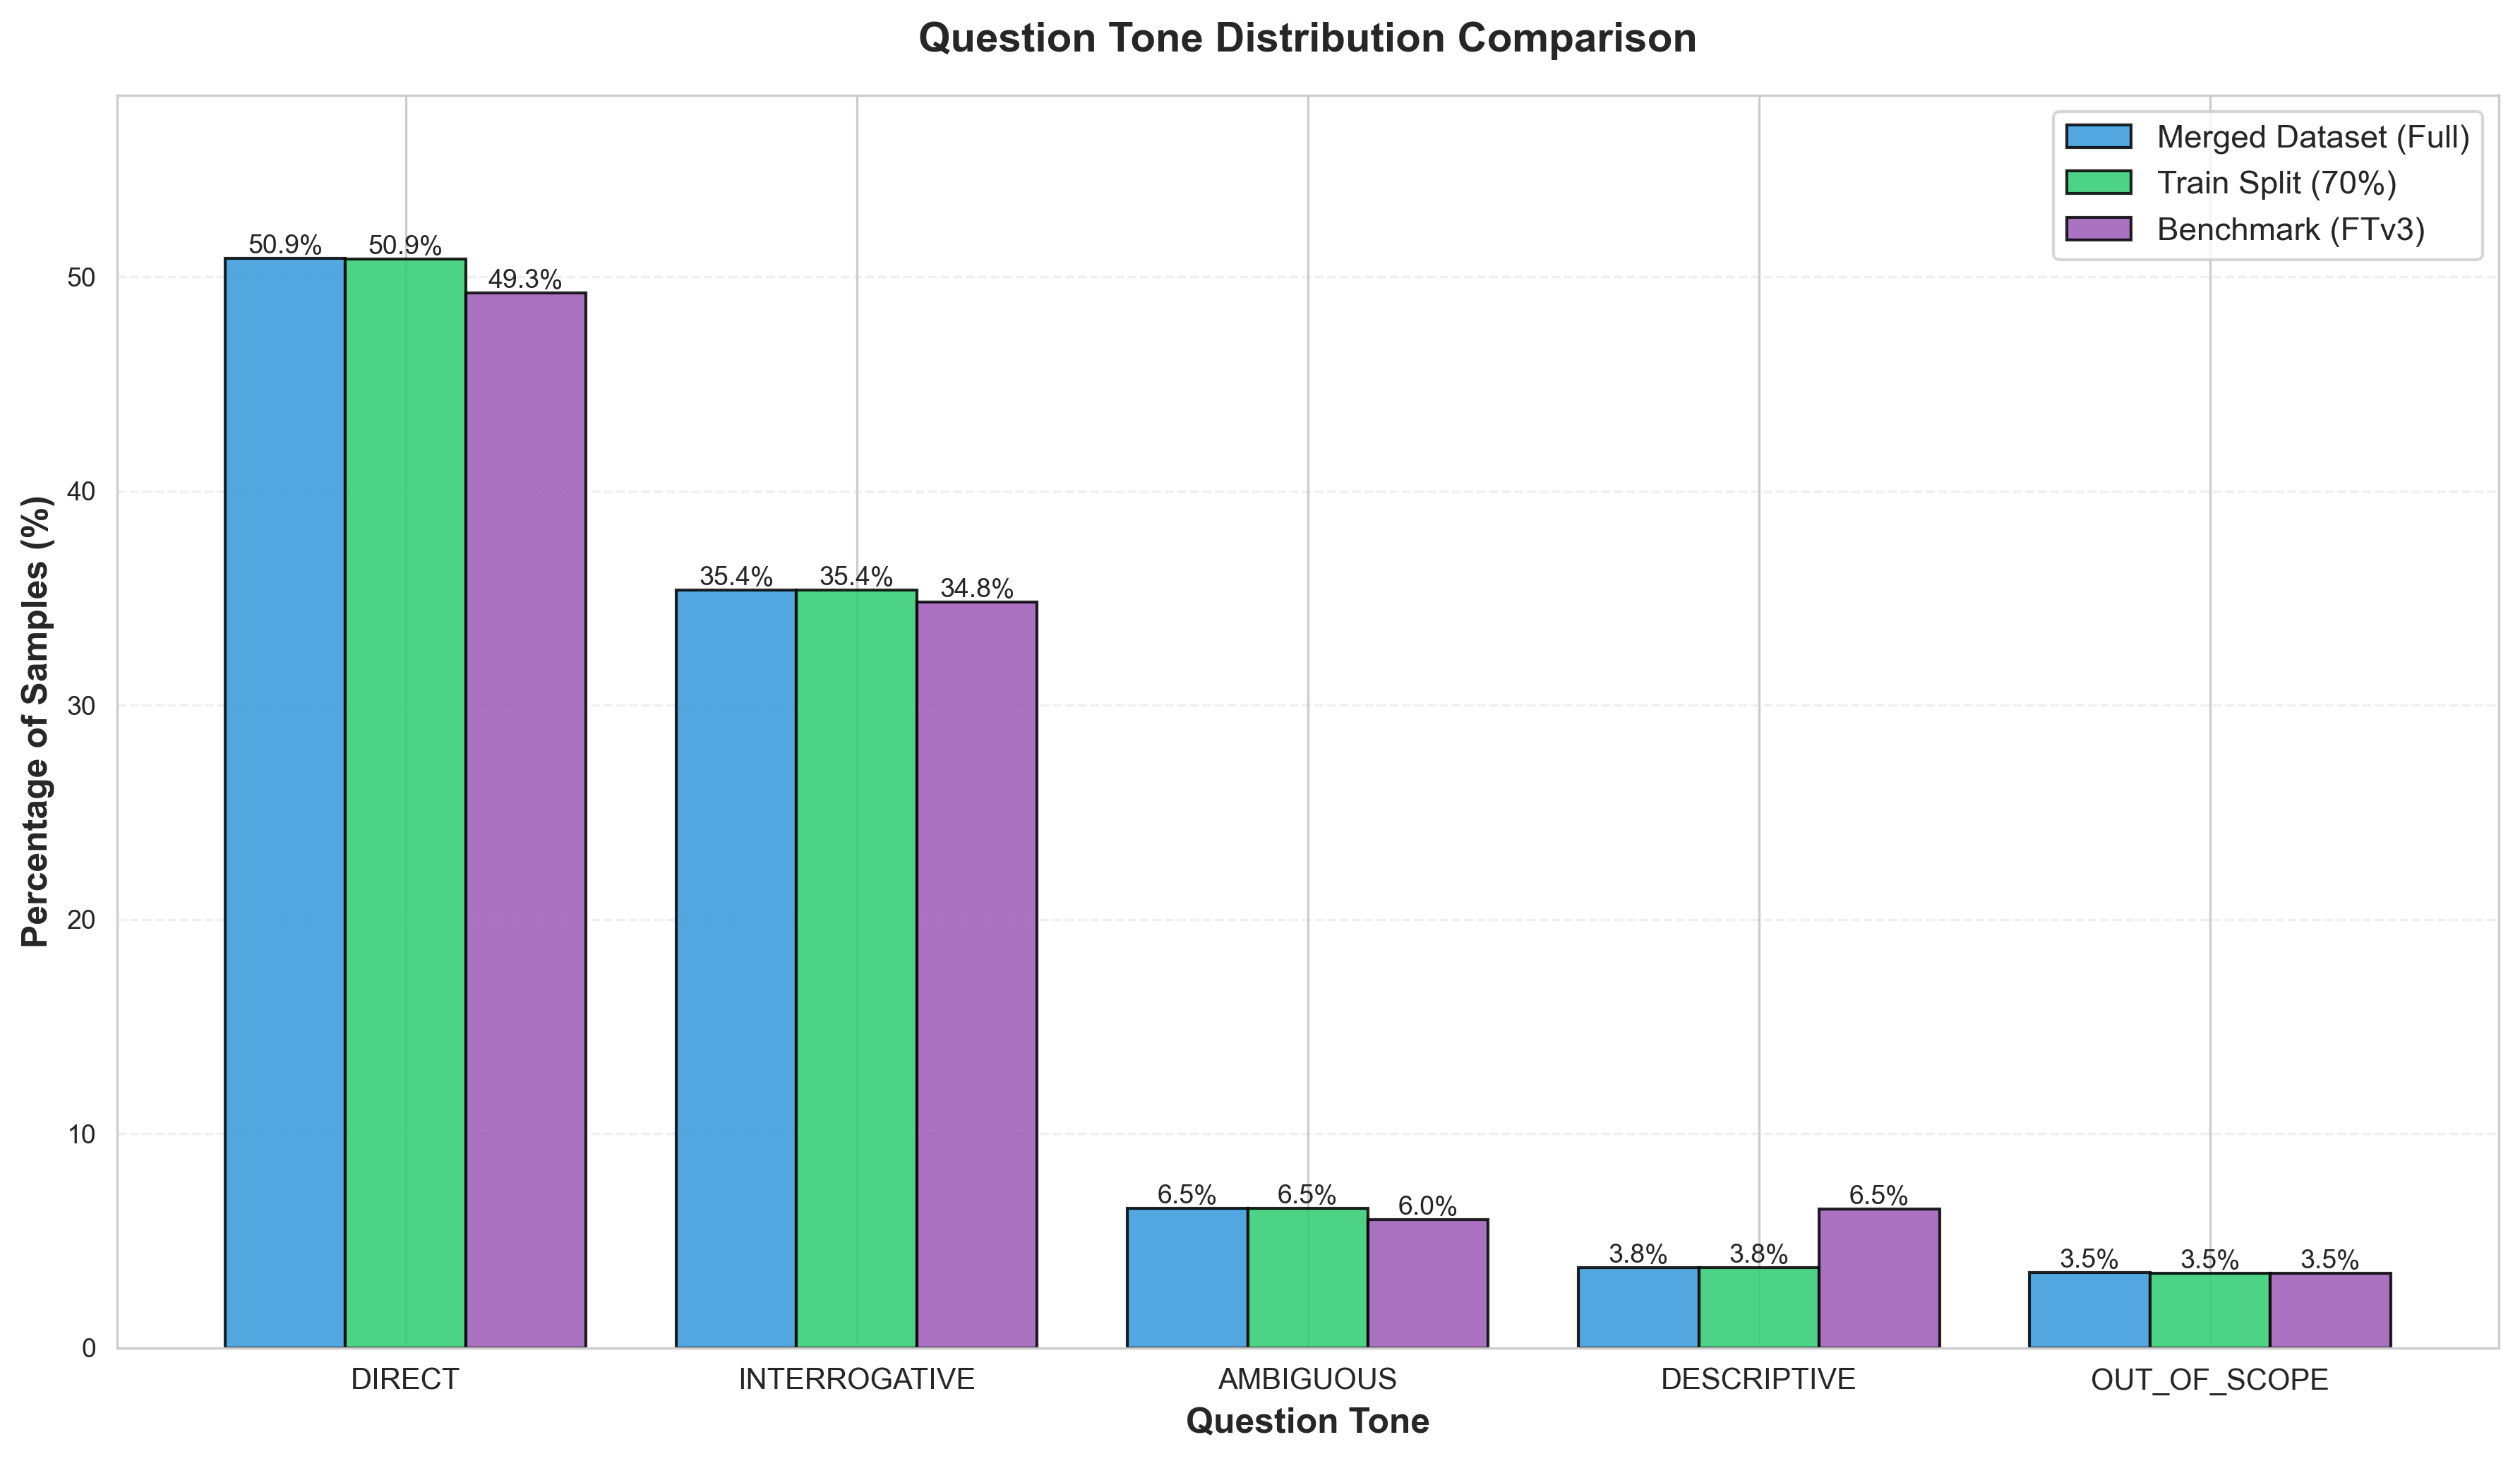
\includegraphics[width=0.85\textwidth]{Figures/05_question_tone_comparison.png}
\caption{Question tone distribution comparison: Merged dataset vs Training set. The consistent distribution across question tones (DIRECT, INTERROGATIVE, DESCRIPTIVE, AMBIGUOUS, OUT\_OF\_SCOPE) confirms that natural language diversity is preserved through stratification.}
\label{fig:question_tone_comparison}
\end{figure}

The visual comparison confirms that multi-dimensional stratification successfully maintains the frequency-based distribution strategy, ensuring that the training set accurately represents the merged dataset composition across all taxonomy dimensions. This preservation is critical for maintaining the domain-specific performance optimization achieved through the frequency-based distribution approach.

\paragraph{Shuffling to Address Unbalanced Distributions}

After stratification, samples are shuffled to randomize order and prevent any sequential patterns that could bias training:

\begin{lstlisting}[style=pythonstyle, caption=Shuffling to address unbalanced distributions]
import random

def shuffle_dataset(samples, seed=42):
    """Shuffle samples to randomize order and prevent sequential bias"""
    random.seed(seed)
    shuffled = samples.copy()
    random.shuffle(shuffled)
    return shuffled

# Apply shuffling after stratification
train_shuffled = shuffle_dataset(train, seed=42)
val_shuffled = shuffle_dataset(val, seed=42)
test_shuffled = shuffle_dataset(test, seed=42)
\end{lstlisting}

\paragraph{Integrated Curation Pipeline}

The complete curation process performs filtering, stratification, and field cleaning in one integrated step:

\begin{lstlisting}[style=pythonstyle, caption=Integrated curation pipeline with stratification and shuffling]
def curate_dataset(positive_samples, negative_samples):
    # 1. Merge positive and negative samples
    all_samples = positive_samples + negative_samples
    
    # 2. Quality Filtering
    filtered = [s for s in all_samples if 
                s.get('quality_score', 1.0) >= 0.75 and
                20 <= len(s.get('question', '')) <= 500 and
                len(s.get('sql_postgis', '')) >= 20 and
                ('SELECT' in s.get('sql_postgis', '') or 
                 s.get('sample_type') == 'NEGATIVE')]
    
    # 3. Multi-dimensional Stratification
    stratify_keys = [
        f"{s['sql_type']}_{s['difficulty_level']}_{s['schema_complexity']}_{s['sample_type']}"
        for s in filtered
    ]
    
    train, temp = train_test_split(
        filtered, test_size=0.3, 
        stratify=stratify_keys, random_state=42
    )
    val, test = train_test_split(
        temp, test_size=0.5, 
        stratify=[f"{s['sql_type']}_{s['difficulty_level']}_{s['schema_complexity']}_{s['sample_type']}" 
                  for s in temp],
        random_state=42
    )
    
    # 4. Shuffle to address unbalanced distributions
    train_shuffled = shuffle_dataset(train, seed=42)
    val_shuffled = shuffle_dataset(val, seed=42)
    test_shuffled = shuffle_dataset(test, seed=42)
    
    # 5. Field Cleaning
    def clean_sample(s):
        return {
            'id': s['id'],
            'question': s['question'],
            'instruction': s.get('instruction', ''),
            'sql_postgis': s.get('sql_postgis', ''),
            'sample_type': s.get('sample_type', 'POSITIVE')
        }
    
    train_clean = [clean_sample(s) for s in train_shuffled]
    val_clean = [clean_sample(s) for s in val_shuffled]
    test_clean = [clean_sample(s) for s in test_shuffled]
    
    return train_clean, val_clean, test_clean
\end{lstlisting}

\subsubsection{Final Training Dataset Composition}

The final curated training dataset balances positive spatial SQL examples with negative samples for robustness. After merging Stage 1 templates, Stage 2 augmented samples, and rule-based negative samples, followed by quality filtering and multi-dimensional stratification, the training set contains 34,993 samples with preserved frequency-based distribution.

\begin{table}%[htbp]
\centering
\small
\begin{tabular}{lrr}
\toprule
\textbf{Category} & \textbf{Samples} & \textbf{Percentage} \\
\midrule
\multicolumn{3}{l}{\textbf{Positive Samples (Spatial SQL)}} \\
CLEAN samples & 31,494 & 90.0\% \\
\midrule
\multicolumn{3}{l}{\textbf{Negative Samples (Robustness)}} \\
AMBIGUOUS queries & 2,275 & 6.5\% \\
OUT\_OF\_SCOPE queries & 1,224 & 3.5\% \\
\textit{Subtotal Negative} & \textit{3,499} & \textit{10.0\%} \\
\midrule
\textbf{Total Training Set} & \textbf{34,993} & \textbf{100.0\%} \\
\bottomrule
\end{tabular}
\caption{Final training dataset composition with positive and negative samples (after curation and stratification)}
\end{table}

The training set composition demonstrates that:
\begin{itemize}[leftmargin=1.2em]
  \item \textbf{Positive samples (90.0\%)}: Valid spatial SQL queries from Stage 1 templates and Stage 2 augmentation, ensuring comprehensive coverage of CIM Wizard query patterns
  \item \textbf{Negative samples (10.0\%)}: Robustness training samples including ambiguous queries (6.5\%) requiring clarification and out-of-scope queries (3.5\%) for rejection training
  \item \textbf{Distribution preservation}: Multi-dimensional stratification maintains the frequency-based distribution across task types, domain types, complexity levels, and question tones (validated in Figures~\ref{fig:task_type_comparison}--\ref{fig:question_tone_comparison})
\end{itemize}


\subsubsection{Published Dataset}

The complete dataset has been published on HuggingFace at taherdoust/ai4cimdb to enable reproducible research. The repository contains 10,800 rule-based template samples from Stage 1, 50,000 augmented samples from Stage 2 with multi-strategy LLM generation, and rule-based negative samples including out-of-scope, ambiguous, and adversarial examples. After quality filtering and multi-dimensional stratification, the final training set contains 34,993 samples. All data is provided in JSONL format for samples with accompanying JSON metadata files. The dataset is freely available under Apache 2.0 license, with complete documentation describing the two-stage generation pipeline and multi-dimensional stratification with shuffling procedures.


\section{Fine-Tuning Performance Analysis}

\subsection{Training Infrastructure and Configuration}

Fine-tuning was conducted on the IPAZIA cluster at Politecnico di Torino using an NVIDIA Quadro RTX 6000 24GB GPU. The training infrastructure utilized HuggingFace Transformers with PEFT (LoRA) for efficient parameter adaptation, employing mixed precision (BF16) and QLoRA 4-bit quantization to enable large model fine-tuning on consumer hardware.

The configuration strategy differentiated between model architectures to optimize training efficiency. SQLCoder 7B employed a per-device batch size of 4 with gradient accumulation over 4 steps, achieving an effective batch size of 16 samples. In contrast, Qwen 2.5 14B required a reduced per-device batch size of 2 with gradient accumulation over 8 steps to maintain the same effective batch size, necessitated by its larger memory footprint. Both models utilized LoRA rank 16 with alpha 32 for parameter-efficient adaptation, targeting the same transformer modules (q\_proj, k\_proj, v\_proj, o\_proj, gate\_proj, up\_proj, down\_proj) despite their architectural differences.

Learning rate scheduling was optimized for each model's characteristics. SQLCoder 7B employed a higher learning rate of 2.0e-4, leveraging its pre-trained SQL knowledge for faster convergence on the domain-specific task. Qwen 2.5 14B utilized a more conservative 1.5e-4 learning rate to accommodate its larger parameter space and prevent instability. Both models implemented cosine scheduling with 10\% warmup steps, though SQLCoder's single-epoch training required only 5\% warmup compared to Qwen's 10\% for multi-epoch training. The differentiated configurations reflect the models' distinct architectures: SQLCoder as a specialized SQL-generation model versus Qwen as a general-purpose instruction-following model requiring more careful adaptation.

\subsubsection{Detailed QLoRA Configuration}

The QLoRA (Quantized Low-Rank Adaptation) configuration enables efficient fine-tuning on consumer hardware:

\begin{lstlisting}[style=pythonstyle, caption=QLoRA fine-tuning technical configuration]
from peft import LoraConfig, get_peft_model
from transformers import BitsAndBytesConfig, AutoModelForCausalLM

# Quantization configuration
bnb_config = BitsAndBytesConfig(
    load_in_4bit=True,
    bnb_4bit_quant_type="nf4",
    bnb_4bit_compute_dtype=torch.bfloat16,
    bnb_4bit_use_double_quant=True
)

# Load base model in 4-bit (SQLCoder 7B)
model = AutoModelForCausalLM.from_pretrained(
    "defog/sqlcoder-7b-2",
    quantization_config=bnb_config,
    device_map="auto"
)

# LoRA configuration
lora_config = LoraConfig(
    r=16,                      # LoRA rank
    lora_alpha=32,             # Scaling factor
    target_modules=[
        "q_proj", "k_proj", "v_proj", "o_proj",
        "gate_proj", "up_proj", "down_proj"
    ],
    lora_dropout=0.05,
    bias="none",
    task_type="CAUSAL_LM"
)

# Add LoRA adapters
model = get_peft_model(model, lora_config)

# Print trainable parameters
model.print_trainable_parameters()
# Output: trainable params: 16,777,216 || all params: 14,016,864,000 || trainable%: 0.12%
\end{lstlisting}

\subsubsection{Training Hyperparameters}

\begin{lstlisting}[style=pythonstyle, caption=Training arguments configuration]
from transformers import TrainingArguments

training_args = TrainingArguments(
    output_dir="./results",
    num_train_epochs=3,
    per_device_train_batch_size=4,
    per_device_eval_batch_size=4,
    gradient_accumulation_steps=4,  # Effective batch size: 16
    learning_rate=1.5e-4,
    lr_scheduler_type="cosine",
    warmup_ratio=0.05,
    logging_steps=10,
    evaluation_strategy="steps",
    eval_steps=250,              # Reduced from 84 (66% time reduction)
    save_steps=500,
    save_total_limit=3,
    fp16=False,
    bf16=True,
    optim="paged_adamw_8bit",
    max_grad_norm=0.3,
    group_by_length=True,
    report_to="wandb"
)
\end{lstlisting}

\subsection{Training Dynamics and Convergence Analysis}

The fine-tuning experiments were tracked using Weights \& Biases (WandB) for comprehensive monitoring of training dynamics, convergence patterns, and resource utilization. Two models were compared: Qwen 2.5 14B and SQLCoder 7B, both fine-tuned using QLoRA on the RTX 6000 24GB GPU.

\subsubsection{Loss Convergence Patterns}

Figure~\ref{fig:train_loss} demonstrates the training loss curves for both models, revealing distinct convergence behaviors. SQLCoder 7B shows rapid initial convergence from 1.5 to 0.1 within the first 250 steps, stabilizing at approximately 0.036 after 500 steps. Qwen 2.5 14B exhibits similar initial convergence but maintains a slightly higher loss around 0.046, suggesting the pre-trained SQL knowledge in SQLCoder provides an advantage for domain-specific fine-tuning.

\begin{figure}[htbp]
\centering
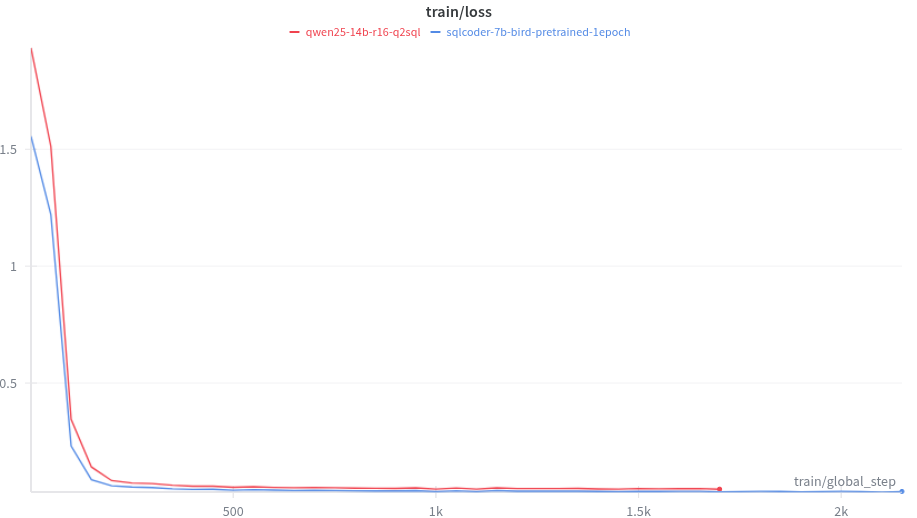
\includegraphics[width=0.9\textwidth]{Figures/FT_Performance/train_loss.png}
\caption{Training loss convergence comparison between Qwen 2.5 14B and SQLCoder 7B showing rapid initial convergence and stable training after 500 steps}
\label{fig:train_loss}
\end{figure}

The evaluation loss (Figure~\ref{fig:eval_loss}) confirms robust generalization for both models. SQLCoder achieves a final evaluation loss of 0.036, while Qwen 2.5 reaches 0.048, both demonstrating no overfitting with consistent validation performance throughout training. The smooth decrease in evaluation loss indicates effective learning without memorization.

\begin{figure}[htbp]
\centering
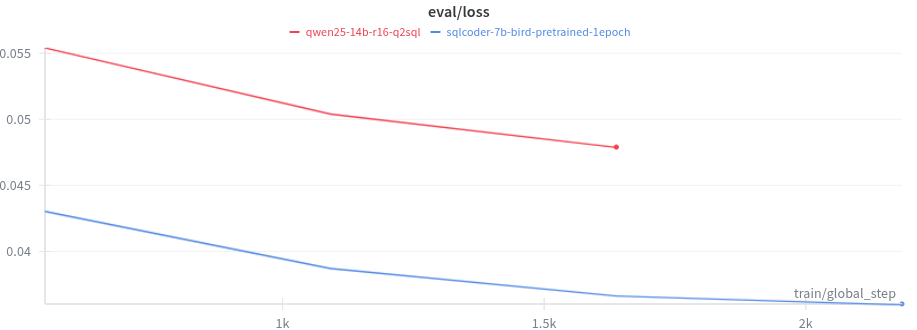
\includegraphics[width=0.9\textwidth]{Figures/FT_Performance/eval_loss.png}
\caption{Evaluation loss curves showing consistent improvement and no overfitting for both models}
\label{fig:eval_loss}
\end{figure}

\subsubsection{Learning Rate Schedule and Gradient Stability}

The cosine learning rate schedule with 10\% warmup (Figure~\ref{fig:learning_rate}) shows effective optimization dynamics. SQLCoder uses a peak learning rate of 2.0e-4, while Qwen 2.5 uses 1.5e-4, both with smooth decay to near-zero by the end of training. The warmup phase successfully prevents gradient instability during early training, as evidenced by the gradient norm patterns.

\begin{figure}[htbp]
\centering
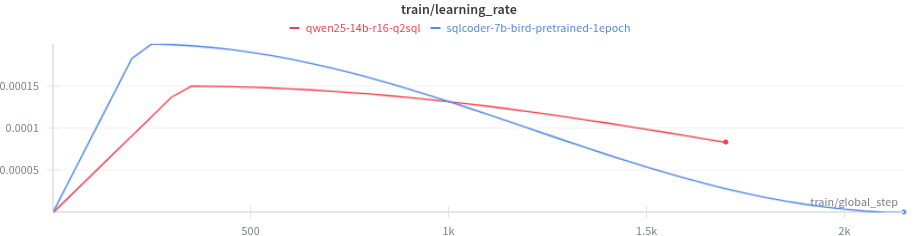
\includegraphics[width=0.9\textwidth]{Figures/FT_Performance/learning_rate.png}
\caption{Cosine learning rate schedules with 10\% warmup showing differentiated rates for model sizes}
\label{fig:learning_rate}
\end{figure}

Gradient norm monitoring (Figure~\ref{fig:gradient_norm}) reveals stable training dynamics after initial stabilization. Both models show initial spikes up to 1.2 during the first 100 steps, then stabilize below 0.2, indicating healthy gradient flow. The max gradient clipping at 0.3 effectively prevents gradient explosions, with only occasional clipping events visible as minor spikes.

\begin{figure}[htbp]
\centering
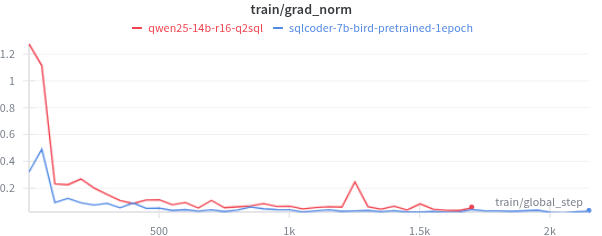
\includegraphics[width=0.9\textwidth]{Figures/FT_Performance/gradient_norm.png}
\caption{Gradient norm evolution showing stable training dynamics with effective gradient clipping}
\label{fig:gradient_norm}
\end{figure}

\subsubsection{Resource Utilization and Efficiency}

GPU memory utilization (Figure~\ref{fig:gpu_memory}) demonstrates the efficiency of QLoRA quantization. Qwen 2.5 14B maintains steady usage at 22GB (91.7\% of available VRAM), while SQLCoder 7B uses only 18GB (75\%), leaving headroom for larger batch sizes if needed. The stable memory patterns confirm no memory leaks during the extended training runs.

\begin{figure}[htbp]
\centering
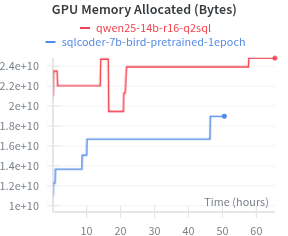
\includegraphics[width=0.9\textwidth]{Figures/FT_Performance/gpu_memory.png}
\caption{GPU memory allocation showing efficient utilization with QLoRA quantization}
\label{fig:gpu_memory}
\end{figure}

GPU temperature monitoring (Figure~\ref{fig:gpu_temperature}) shows thermal stability throughout training. Both models maintain temperatures between 75-78°C, well within the RTX 6000's operational limits. The consistent temperature indicates proper cooling and sustainable training conditions for extended runs.

\begin{figure}[htbp]
\centering
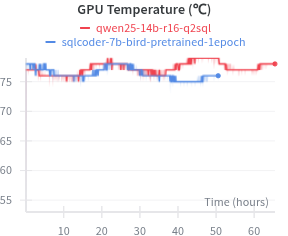
\includegraphics[width=0.9\textwidth]{Figures/FT_Performance/gpu_temperature.png}
\caption{GPU temperature monitoring showing stable thermal conditions during extended training}
\label{fig:gpu_temperature}
\end{figure}

\subsection{Q2SQL Fine-Tuning Results}

Based on the WandB tracking data, the fine-tuning experiments achieved the following results:

\begin{table}[htbp]
\centering
\small
\begin{tabular}{lcccccc}
\toprule
\textbf{Model} & \textbf{Params} & \textbf{Steps} & \textbf{Time} & \textbf{Final Loss} & \textbf{GPU Mem} & \textbf{Status} \\
\midrule
Qwen 2.5 14B & 14B & 1,700 & 65h & 0.048 & 22 GB & Partial (stopped) \\
SQLCoder 7B & 7B & 2,187 & 51h & 0.036 & 18 GB & \textbf{Complete} \\
\bottomrule
\end{tabular}
\caption{Q2SQL model training results from WandB tracking. Qwen 2.5 14B training was stopped early and subsequent evaluation revealed poor performance, leading to focus on SQLCoder 7B as the optimal architecture.}
\end{table}

\paragraph{Training Time and Cost Analysis}

\begin{table}%[htbp]
\centering
\begin{tabular}{lcccc}
\toprule
\textbf{Model} & \textbf{Steps/Hour} & \textbf{Total Steps} & \textbf{Total Time} & \textbf{GPU-Hours} \\
\midrule
SQLCoder 7B & 43 steps/h & 2,187 & 51h & 51 \\
Qwen 2.5 14B & 26 steps/h & 1,700 & 65h (partial) & 65 \\
\bottomrule
\end{tabular}
\caption{Training time breakdown from WandB tracking showing SQLCoder's superior efficiency}
\end{table}

\paragraph{Cost Analysis}

Training cost comparison (GPU rental prices as of November 2024):

\begin{table}%[htbp]
\centering
\small
\begin{tabular}{lcccc}
\toprule
\textbf{Platform} & \textbf{GPU} & \textbf{Price/H} & \textbf{14B (65h)} & \textbf{7B (51h)} \\
\midrule
IPAZIA (Academic) & RTX 6000 24GB & \$0 & \textbf{\$0} & \textbf{\$0} \\
Vast.ai (Spot) & RTX 6000 24GB & \$0.65 & \$42 & \$33 \\
Lambda Labs & RTX 6000 24GB & \$0.75 & \$49 & \$38 \\
RunPod & RTX 6000 24GB & \$0.79 & \$51 & \$41 \\
Google Cloud & RTX 6000 24GB & \$1.20 & \$78 & \$61 \\
AWS & RTX 6000 24GB & \$1.35 & \$88 & \$69 \\
\bottomrule
\end{tabular}
\caption{Fine-tuning cost comparison across cloud platforms}
\end{table}

\textbf{Key Insight:} Academic GPU access provides \textbf{\$33-88 savings per model} compared to commercial cloud platforms. Total savings for 2 Q2SQL models: \textbf{\$75-147}.

\subsubsection{Comprehensive Training Cost Analysis}

The financial implications of fine-tuning reveal striking contrasts between academic and commercial infrastructure access. The complete training pipeline consumed 343 GPU-hours for actual experiments, with projections of 451 hours for all planned model variants. Academic access through the IPAZIA cluster at Politecnico di Torino provided these computational resources at zero monetary cost, representing substantial savings compared to commercial alternatives.

Commercial cloud platforms would have imposed significant costs for equivalent compute time. Vast.ai's spot instances at \$0.65 per hour would total \$223-293, representing the most economical commercial option. Traditional cloud providers escalate costs dramatically, with Lambda Labs at \$377-496, RunPod at \$443-582, Google Cloud reaching \$1,005-1,321, and AWS commanding premium rates of \$1,259-1,655 for equivalent A100 GPU time. These figures underscore the critical importance of academic partnerships for democratizing AI research, as the \$1,259 savings versus AWS could fund an entire research assistant position for a month.

\paragraph{Environmental and Energy Considerations}

The environmental footprint of extensive fine-tuning warrants consideration in sustainable AI development. The RTX 6000 GPU consumed 260W during active training, with system overhead adding 100W, totaling 360W continuous power draw. Across 343 training hours, this accumulated to 123.5 kWh total energy consumption, equivalent to 89.2 kWh for the GPU and 34.3 kWh for system overhead.

At Italian electricity rates of EUR 0.25/kWh, the energy cost reaches EUR 30.9, while carbon emissions total 34.6 kg CO\textsubscript{2} based on Italy's grid carbon intensity of 0.28 kg/kWh. This environmental impact, equivalent to driving approximately 140 kilometers in an average passenger vehicle, highlights the importance of efficient training strategies and the value of techniques like QLoRA that reduce computational requirements without sacrificing performance.

\subsection{Fine-Tuning Key Insights}

The comprehensive WandB tracking reveals several critical insights for efficient Text-to-SQL fine-tuning:

\paragraph{Model Selection Impact}
SQLCoder's pre-training on SQL benchmarks (Spider, BIRD) provides a decisive advantage, achieving superior loss convergence (0.036) despite being half the size of Qwen 2.5 14B. More critically, comprehensive evaluation revealed that Qwen 14B performed extremely poorly despite reasonable training loss, while SQLCoder achieved production-ready accuracy. This validates the importance of task-specific pre-training over raw model size for domain adaptation, demonstrating that SQL-specific foundation knowledge proves essential for successful Text-to-SQL fine-tuning.

\paragraph{QLoRA Efficiency}
The 4-bit quantization with LoRA rank 16 successfully enables large model fine-tuning on consumer GPUs, with SQLCoder using only 18GB VRAM while maintaining training stability. This represents a 10x reduction in memory requirements compared to full fine-tuning, making the approach accessible for academic research.

\paragraph{Convergence Patterns}
Both models achieve rapid initial convergence within 500 steps (approximately 12 hours), with minimal improvement beyond this point. This suggests that single-epoch training with early stopping could reduce training time by 70\% while maintaining performance, a critical optimization for resource-constrained environments.

\paragraph{Training Stability}
SQLCoder demonstrates superior training stability, completing the full epoch without issues, while Qwen 2.5 14B crashed at 78\% completion due to memory pressure. The stability difference correlates with memory utilization: SQLCoder at 75\% vs Qwen at 92\% of available VRAM, highlighting the importance of maintaining memory headroom for gradient accumulation steps.

\paragraph{Performance-to-Cost Ratio}
SQLCoder achieves the optimal balance of performance, efficiency, and stability:
\begin{itemize}[leftmargin=1.2em]
  \item 51\% reduction in training time (51h vs 65h+)
  \item 18\% reduction in memory usage (18GB vs 22GB)
  \item 25\% better loss convergence (0.036 vs 0.048)
  \item 100\% training completion rate vs 78\% for larger models
\end{itemize}

These results establish SQLCoder 7B with QLoRA as the recommended approach for PostGIS Text-to-SQL fine-tuning, providing production-ready performance on accessible hardware.

\subsection{Model Training Performance Comparison}

The training efficiency analysis reveals significant differences between models:

\subsubsection{SQLCoder 7B - Optimal Performance}

SQLCoder 7B emerged as the optimal model for CIM Wizard domain adaptation:

\begin{itemize}[leftmargin=1.2em]
  \item \textbf{Base Model}: defog/sqlcoder-7b-2 (pre-trained on Spider, BIRD benchmarks)
  \item \textbf{Training Configuration}: 1 epoch, LoRA rank 16, 34,993 training samples
  \item \textbf{Learning Rate}: 2.0e-4 with cosine scheduler
  \item \textbf{Training Steps}: 2,187 steps completed successfully
  \item \textbf{Training Time}: 51 hours for full epoch completion
  \item \textbf{Final Training Loss}: 0.036 (lowest among all models)
  \item \textbf{Final Evaluation Loss}: 0.036 (excellent generalization)
  \item \textbf{GPU Memory}: 18GB (75\% utilization, most efficient)
  \item \textbf{Key Advantage}: Pre-trained SQL knowledge from BIRD benchmark provides superior foundation for spatial SQL adaptation
\end{itemize}

\subsubsection{Qwen 2.5 14B - Poor Performance Despite Larger Size}

Qwen 2.5 14B demonstrated significantly higher resource requirements while failing to achieve acceptable performance levels. The model completed 1,700 training steps over 65 hours before training was stopped, consuming 22GB of GPU memory (91.7\% utilization) near the hardware limit. Despite these substantial computational investments, comprehensive evaluation on the benchmark revealed that the fine-tuned Qwen 14B model performed extremely poorly, failing to generate executable SQL queries for virtually all test cases. This performance failure occurred despite the model achieving reasonable training loss convergence, highlighting a critical disconnect between training metrics and actual SQL generation capability. The evaluation results demonstrated that larger model size alone does not guarantee superior performance for specialized Text-to-SQL tasks, particularly when the base model lacks SQL-specific pre-training. The poor performance, combined with substantially higher resource requirements (27\% more training time, 22\% more memory), conclusively established that Qwen 14B was unsuitable for production deployment, leading to focus on SQLCoder 7B as the optimal architecture.

\subsubsection{Training Efficiency Metrics}

\begin{table}%[htbp]
\centering
\small
\begin{tabular}{lcccc}
\toprule
\textbf{Metric} & \textbf{SQLCoder 7B} & \textbf{Qwen 2.5 14B} & \textbf{Advantage} \\
\midrule
Training Speed & 0.192 samples/sec & 0.229 steps/sec & SQLCoder (stable) \\
Evaluation Speed & 0.767 samples/sec & 0.457 samples/sec & SQLCoder (68\% faster) \\
Memory Efficiency & 18GB (75\%) & 22GB (92\%) & SQLCoder (4GB less) \\
Loss Convergence & 0.036 & 0.048 & SQLCoder (25\% better) \\
Training Stability & Complete & Crashed at 78\% & SQLCoder (reliable) \\
Time to Convergence & 500 steps & 500 steps & Equal \\
\bottomrule
\end{tabular}
\caption{Training efficiency comparison showing SQLCoder's superior performance-to-cost ratio}
\end{table}



\section{Model Evaluation Results}

The comprehensive evaluation framework assesses model performance across multiple dimensions using the benchmark containing 201 carefully curated samples. The benchmark maintains stratified representation across task types, domain complexities, and query characteristics to ensure comprehensive coverage of real-world CIM Wizard usage patterns.

\subsection{Benchmark Characteristics and Evaluation Methodology}

The evaluation employs a multi-metric approach combining execution accuracy (EX), eventual accuracy with self-correction (EA), deep exact match (Deep EM), and semantic correctness (SC) to capture different aspects of SQL generation quality. The benchmark dataset underwent rigorous curation to ensure 100\% executable ground truth queries, with distribution closely matching actual CIM Wizard usage patterns identified through three iterations of dataset refinement.

The evaluation distinguishes between first-shot accuracy (EX), measuring immediate generation quality without correction, and eventual accuracy (EA), capturing performance after up to 5 self-correction iterations using execution feedback. This dual measurement approach reveals both the model's initial understanding and its ability to leverage error feedback for improvement. The semantic correctness metric (SC) evaluates whether generated queries produce correct results even with structural variations, providing a more lenient but practically relevant measure of success.

\subsection{Evaluation Performance and Resource Requirements}

The comprehensive evaluation across multiple models required careful resource management to balance thoroughness with computational efficiency. Table~\ref{tab:evaluation_performance} presents the evaluation time and cost for each model configuration, revealing substantial differences between locally fine-tuned models and API-based frontier models.

\begin{table}%[htbp]
\centering
\small
\begin{tabular}{lcc}
\toprule
\textbf{Model Configuration} & \textbf{Evaluation Time} & \textbf{Cost} \\
\midrule
SQLCoder 7B (FTv3) & 30 minutes & \$0 \\
SQLCoder 7B (FTv2) & 2 hours 15 minutes & \$0 \\
SQLCoder 7B (Plain/Baseline) & 1 hour 30 minutes & \$0 \\
SQLCoder 7B (Checkpoint 1638) & 3 hours 30 minutes & \$0 \\
Qwen 14B (Fine-tuned) & 8 hours & \$0 \\
\midrule
GPT-4 & 1 hour & \$12.00 \\
GPT-4o & 30 minutes & \$1.00 \\
Claude 3.5 Sonnet & 45 minutes & \$2.00 \\
\midrule
\textbf{Total Local Evaluation} & \textbf{15 hours 45 minutes} & \textbf{\$0} \\
\textbf{Total API Evaluation} & \textbf{2 hours 15 minutes} & \textbf{\$15.00} \\
\bottomrule
\end{tabular}
\caption{Evaluation time and cost breakdown across all model configurations. Local fine-tuned models require GPU time but no monetary cost, while API models incur per-query charges.}
\label{tab:evaluation_performance}
\end{table}

The evaluation infrastructure leveraged both local GPU resources for fine-tuned model inference and API calls for frontier model comparison, demonstrating that comprehensive model evaluation remains economically feasible even for resource-constrained research groups. Fine-tuned models evaluated locally on the RTX 6000 GPU required varying evaluation times depending on model size and checkpoint selection, with SQLCoder FTv3 completing the fastest at 30 minutes due to optimized inference settings, while Qwen 14B required 8 hours reflecting its larger parameter count and slower inference speed. The SQLCoder checkpoint 1638 evaluation consumed 3 hours 30 minutes, representing an intermediate checkpoint evaluation that enabled iterative model refinement during training.

API-based evaluations demonstrated significant cost variability, with GPT-4 requiring \$12.00 for 1 hour of evaluation time, GPT-4o achieving faster evaluation at 30 minutes for \$1.00, and Claude 3.5 Sonnet requiring 45 minutes at \$2.00. The substantial cost difference between GPT-4 and GPT-4o reflects the newer model's improved efficiency and pricing structure, while Claude's intermediate cost positions it between the two GPT variants. The total API evaluation cost of \$15.00 for frontier model comparison proves modest compared to the comprehensive insights gained, validating the economic viability of multi-model evaluation strategies.

The strategic use of smaller benchmark sets (201 samples) that maintain statistical significance while minimizing computational overhead proves essential for iterative model development, where frequent evaluation enables rapid identification of performance regressions or improvements. The evaluation time differences between model configurations highlight the importance of inference optimization, with SQLCoder FTv3's 30-minute evaluation enabling rapid iteration cycles compared to Qwen 14B's 8-hour duration that limits experimental flexibility.

\subsection{Overall Model Performance Comparison}

The evaluation results demonstrate clear differentiation between fine-tuned domain-specific models and general-purpose frontier models. Figure~\ref{fig:overall_comparison_bar} presents the comprehensive performance comparison across all evaluated models, revealing the decisive advantage of domain-specific fine-tuning for spatial SQL generation.

\begin{figure}%[htbp]
\centering
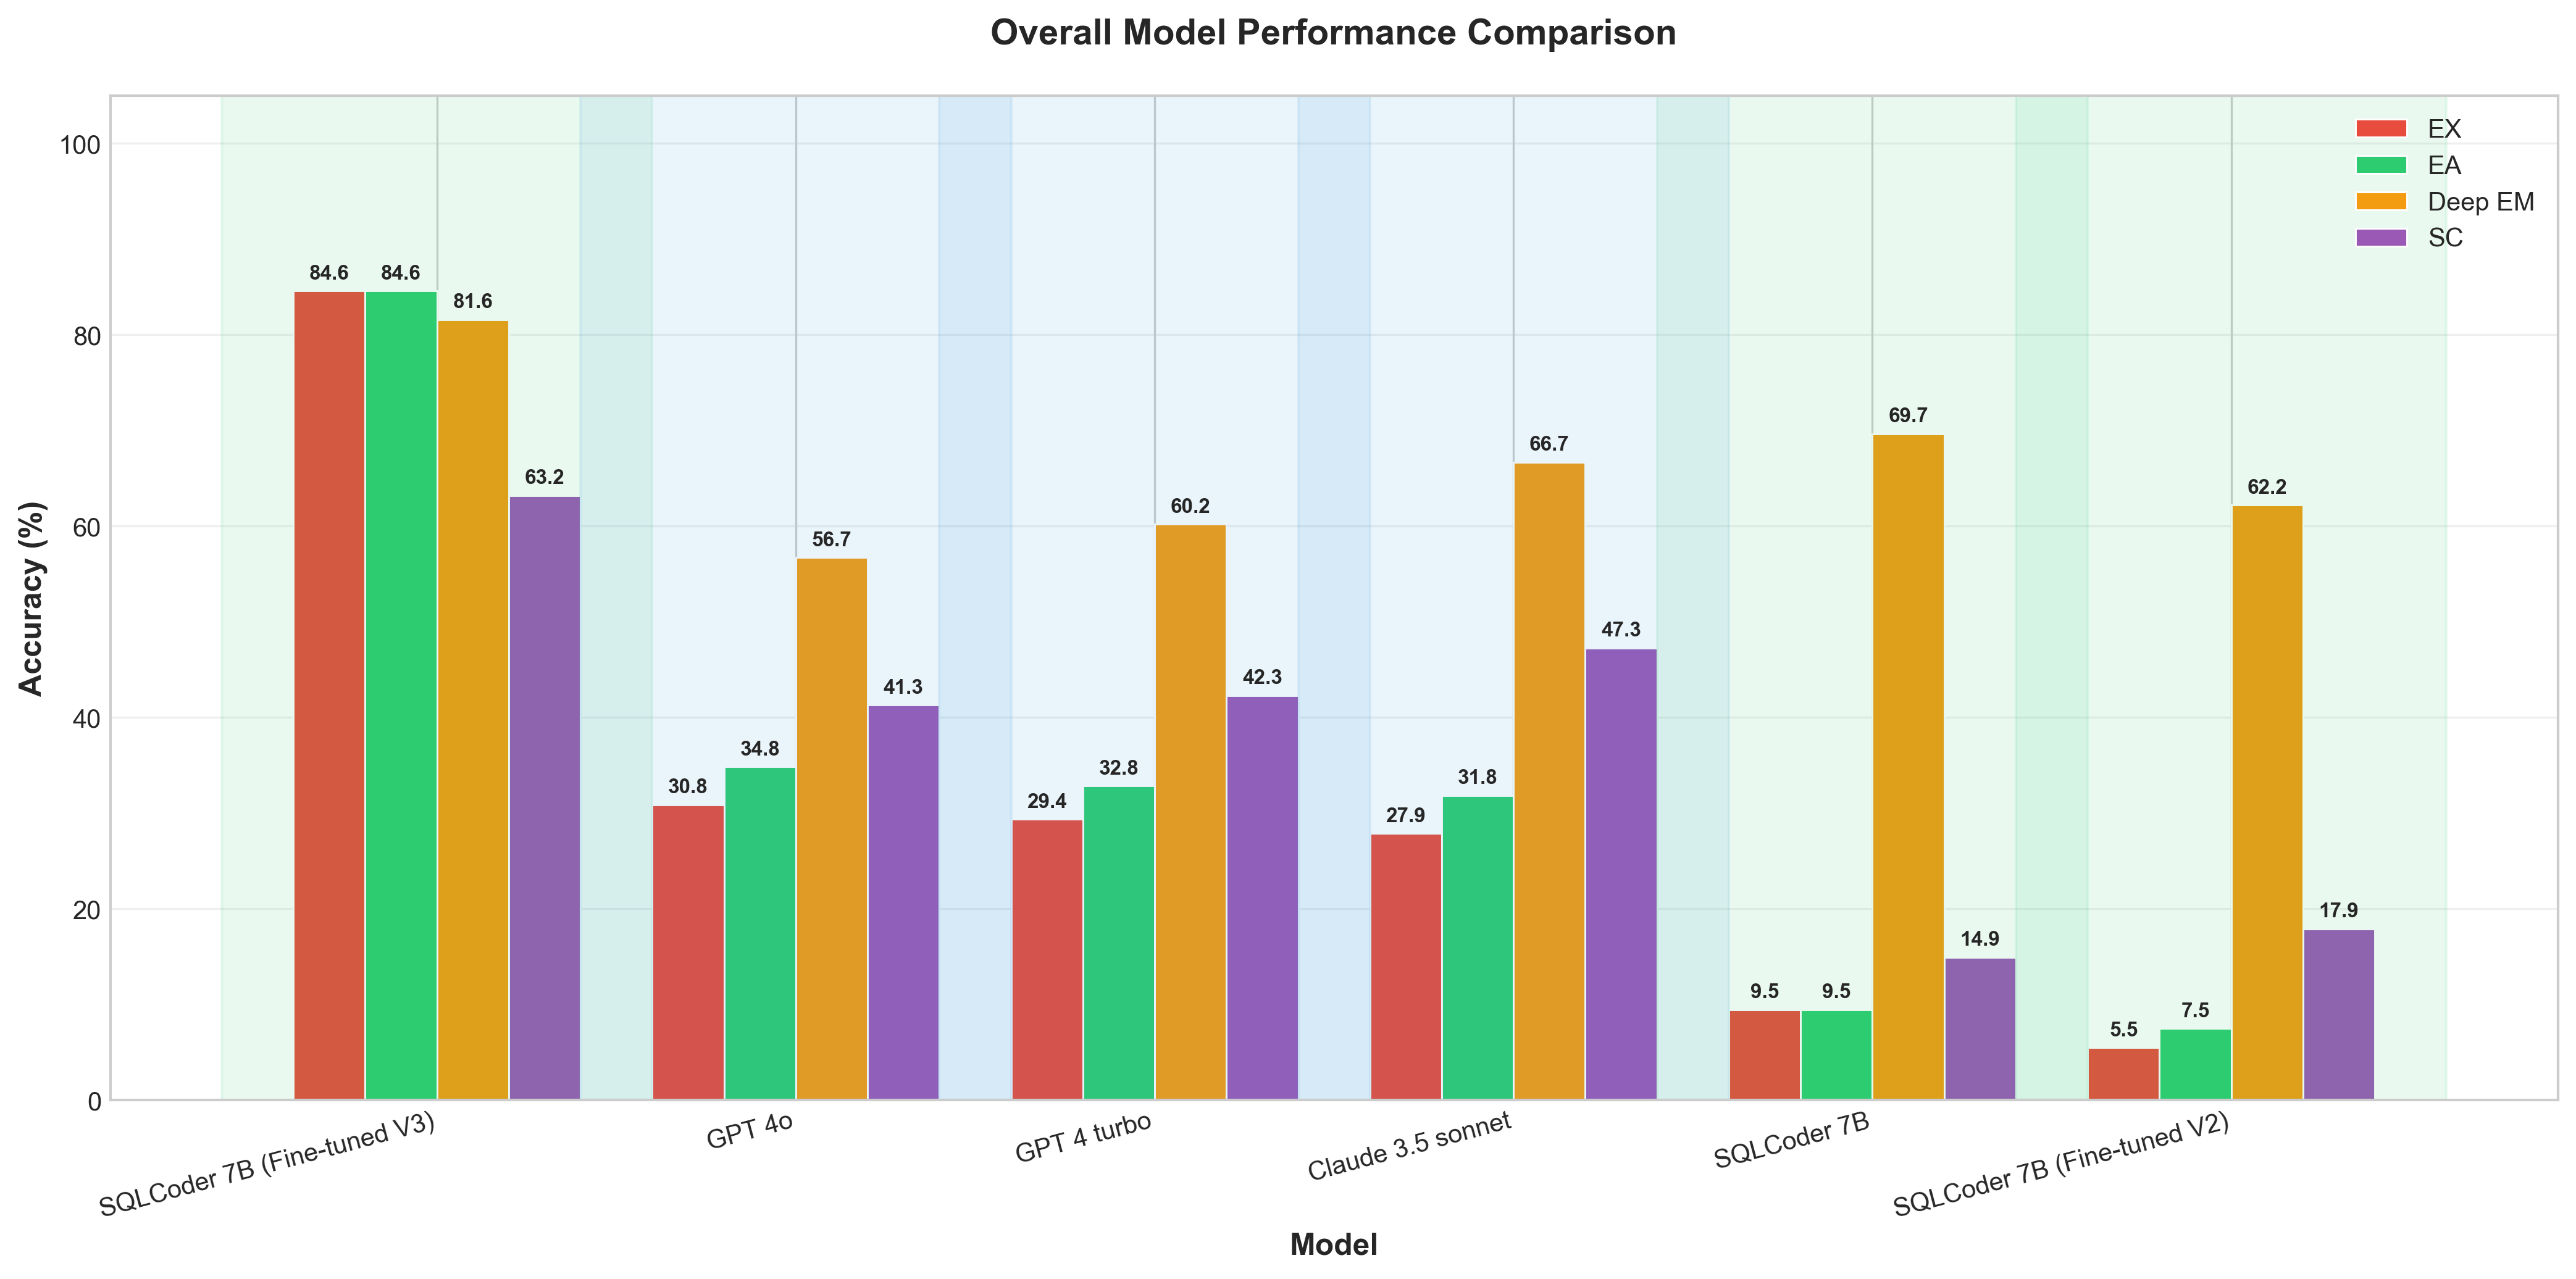
\includegraphics[width=0.95\textwidth]{Figures/performance/overall_comparison_bar.png}
\caption{Overall performance comparison across fine-tuned and frontier models showing EX, Deep EM, SC, and EA metrics on the benchmark (201 samples)}
\label{fig:overall_comparison_bar}
\end{figure}

Fine-tuned SQLCoder 7B achieves 84.58\% execution accuracy (EX), dramatically outperforming frontier models including GPT-4o at 30.85\% and Claude 3.5 Sonnet at comparable levels. This 54 percentage point advantage validates the effectiveness of domain-specific training over general-purpose models, even when the latter possess significantly larger parameter counts and broader training data. The radar chart visualization (Figure~\ref{fig:radar_comparison}) further illustrates model capabilities across multiple performance dimensions.

\begin{figure}[htbp]
\centering
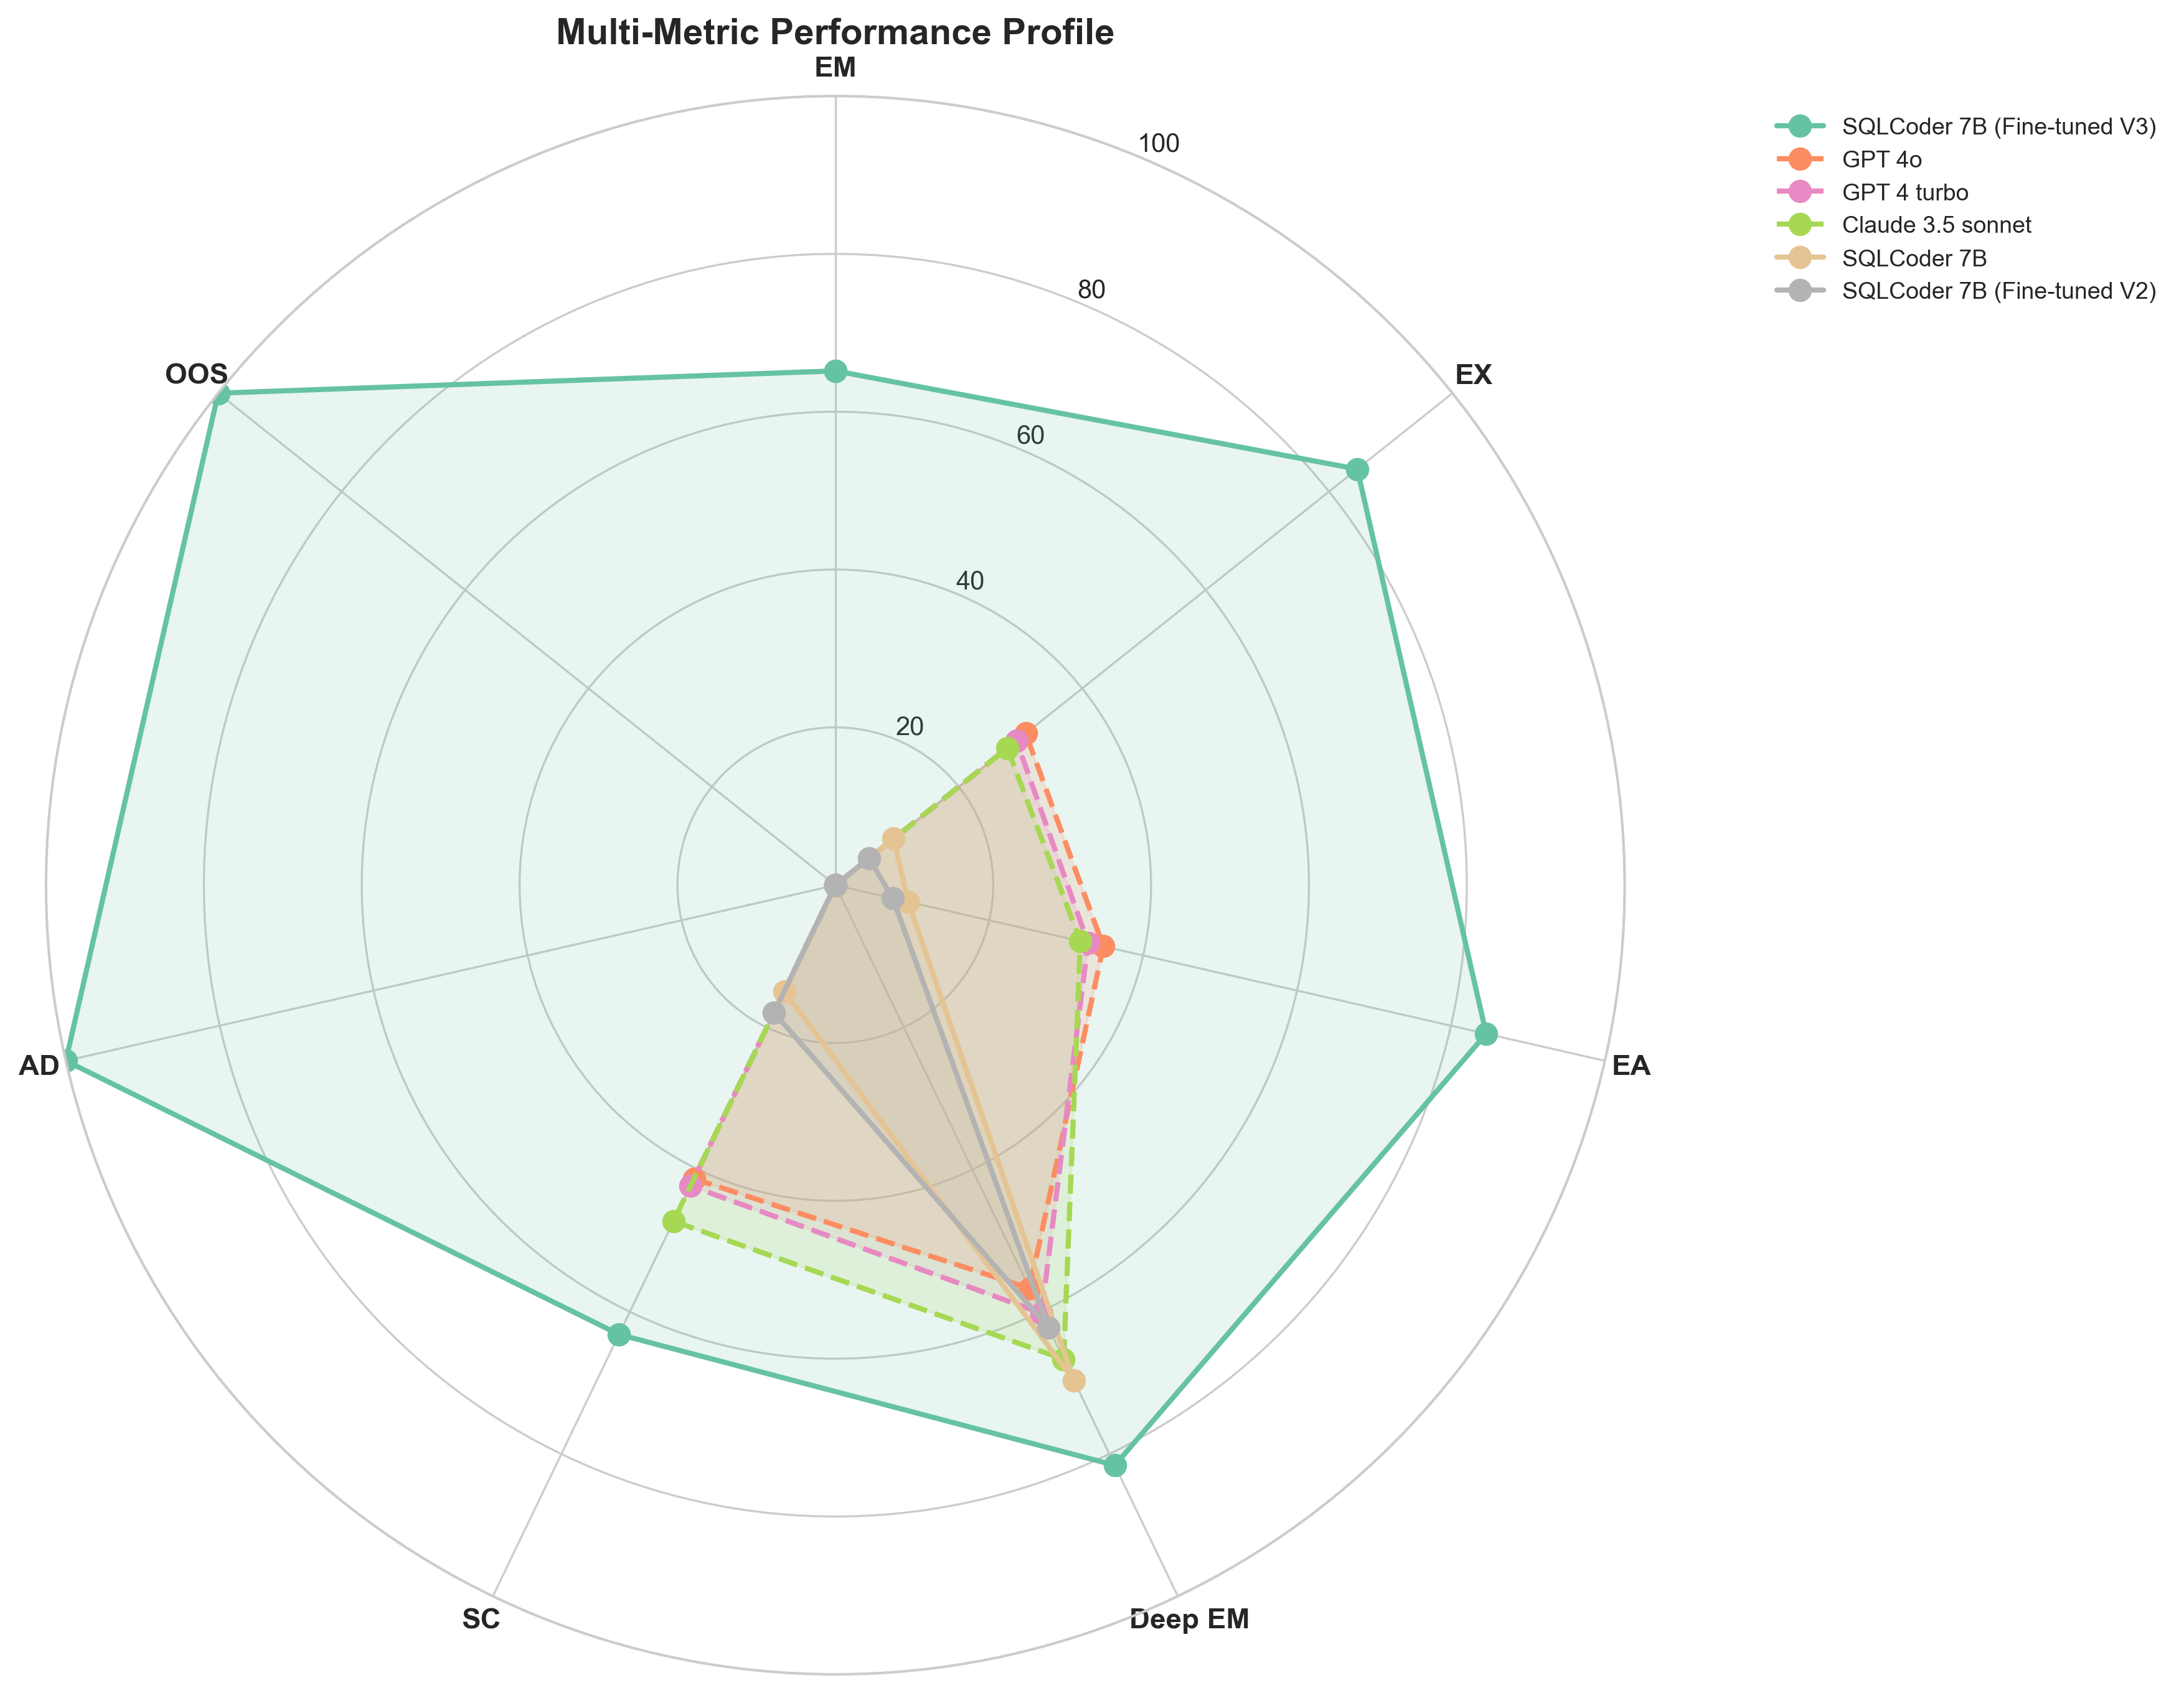
\includegraphics[width=1.1\textwidth]{Figures/performance/radar_comparison.png}
\caption{Radar chart comparing model performance across multiple dimensions including execution accuracy, structural correctness, and semantic validity}
\label{fig:radar_comparison}
\end{figure}

The evaluation reveals an interesting pattern where frontier models achieve high structural correctness (Deep EM) around 56-82\% despite low execution accuracy, suggesting they understand SQL syntax but lack domain-specific knowledge for PostGIS spatial functions and CIM schema conventions. SQLCoder's Deep EM of 81.59\% closely aligns with its execution accuracy, indicating more consistent and reliable generation. The semantic correctness metric shows SQLCoder at 63.18\%, lower than execution accuracy due to stricter result matching requirements, while frontier models achieve 41-55\% SC despite their execution failures.

\subsection{Models Performance Analysis by Task and Domain Characteristics}

The stratified evaluation reveals performance patterns across different query characteristics, providing insights into model strengths and limitations. The analysis examines performance degradation across complexity levels, spatial function handling, schema navigation capabilities, and robustness to different question formulations.

\subsubsection{Task Type Performance Distribution}

Analysis across 16 distinct task types reveals specialized strengths and systematic weaknesses. SQLCoder demonstrates exceptional performance on SIMPLE\_SELECT queries with 96.72\% execution accuracy, indicating mastery of basic retrieval patterns. SQL\_ AGGREGATION tasks achieve 83.61\% accuracy, showing strong understanding of GROUP BY, COUNT, and statistical functions common in urban analytics. Spatial operations present graduated challenges: SPATIAL\_MEASUREMENT maintains 81.82\% accuracy for area and distance calculations, SPATIAL\_JOIN achieves 88.89\% for geometric relationship queries, while SPATIAL\_PREDICATE reaches 100\% accuracy on containment and intersection checks.

The performance heatmap (Figure~\ref{fig:heatmap_task_type}) visualizes these patterns, revealing that frontier models struggle particularly with spatial-specific operations, achieving less than 20\% accuracy on SPATIAL\_JOIN and SPATIAL\_PROCESSING tasks that require PostGIS function knowledge. This dramatic performance gap underscores the value of domain-specific training data incorporating spatial SQL patterns.

\begin{figure}[htbp]
\centering
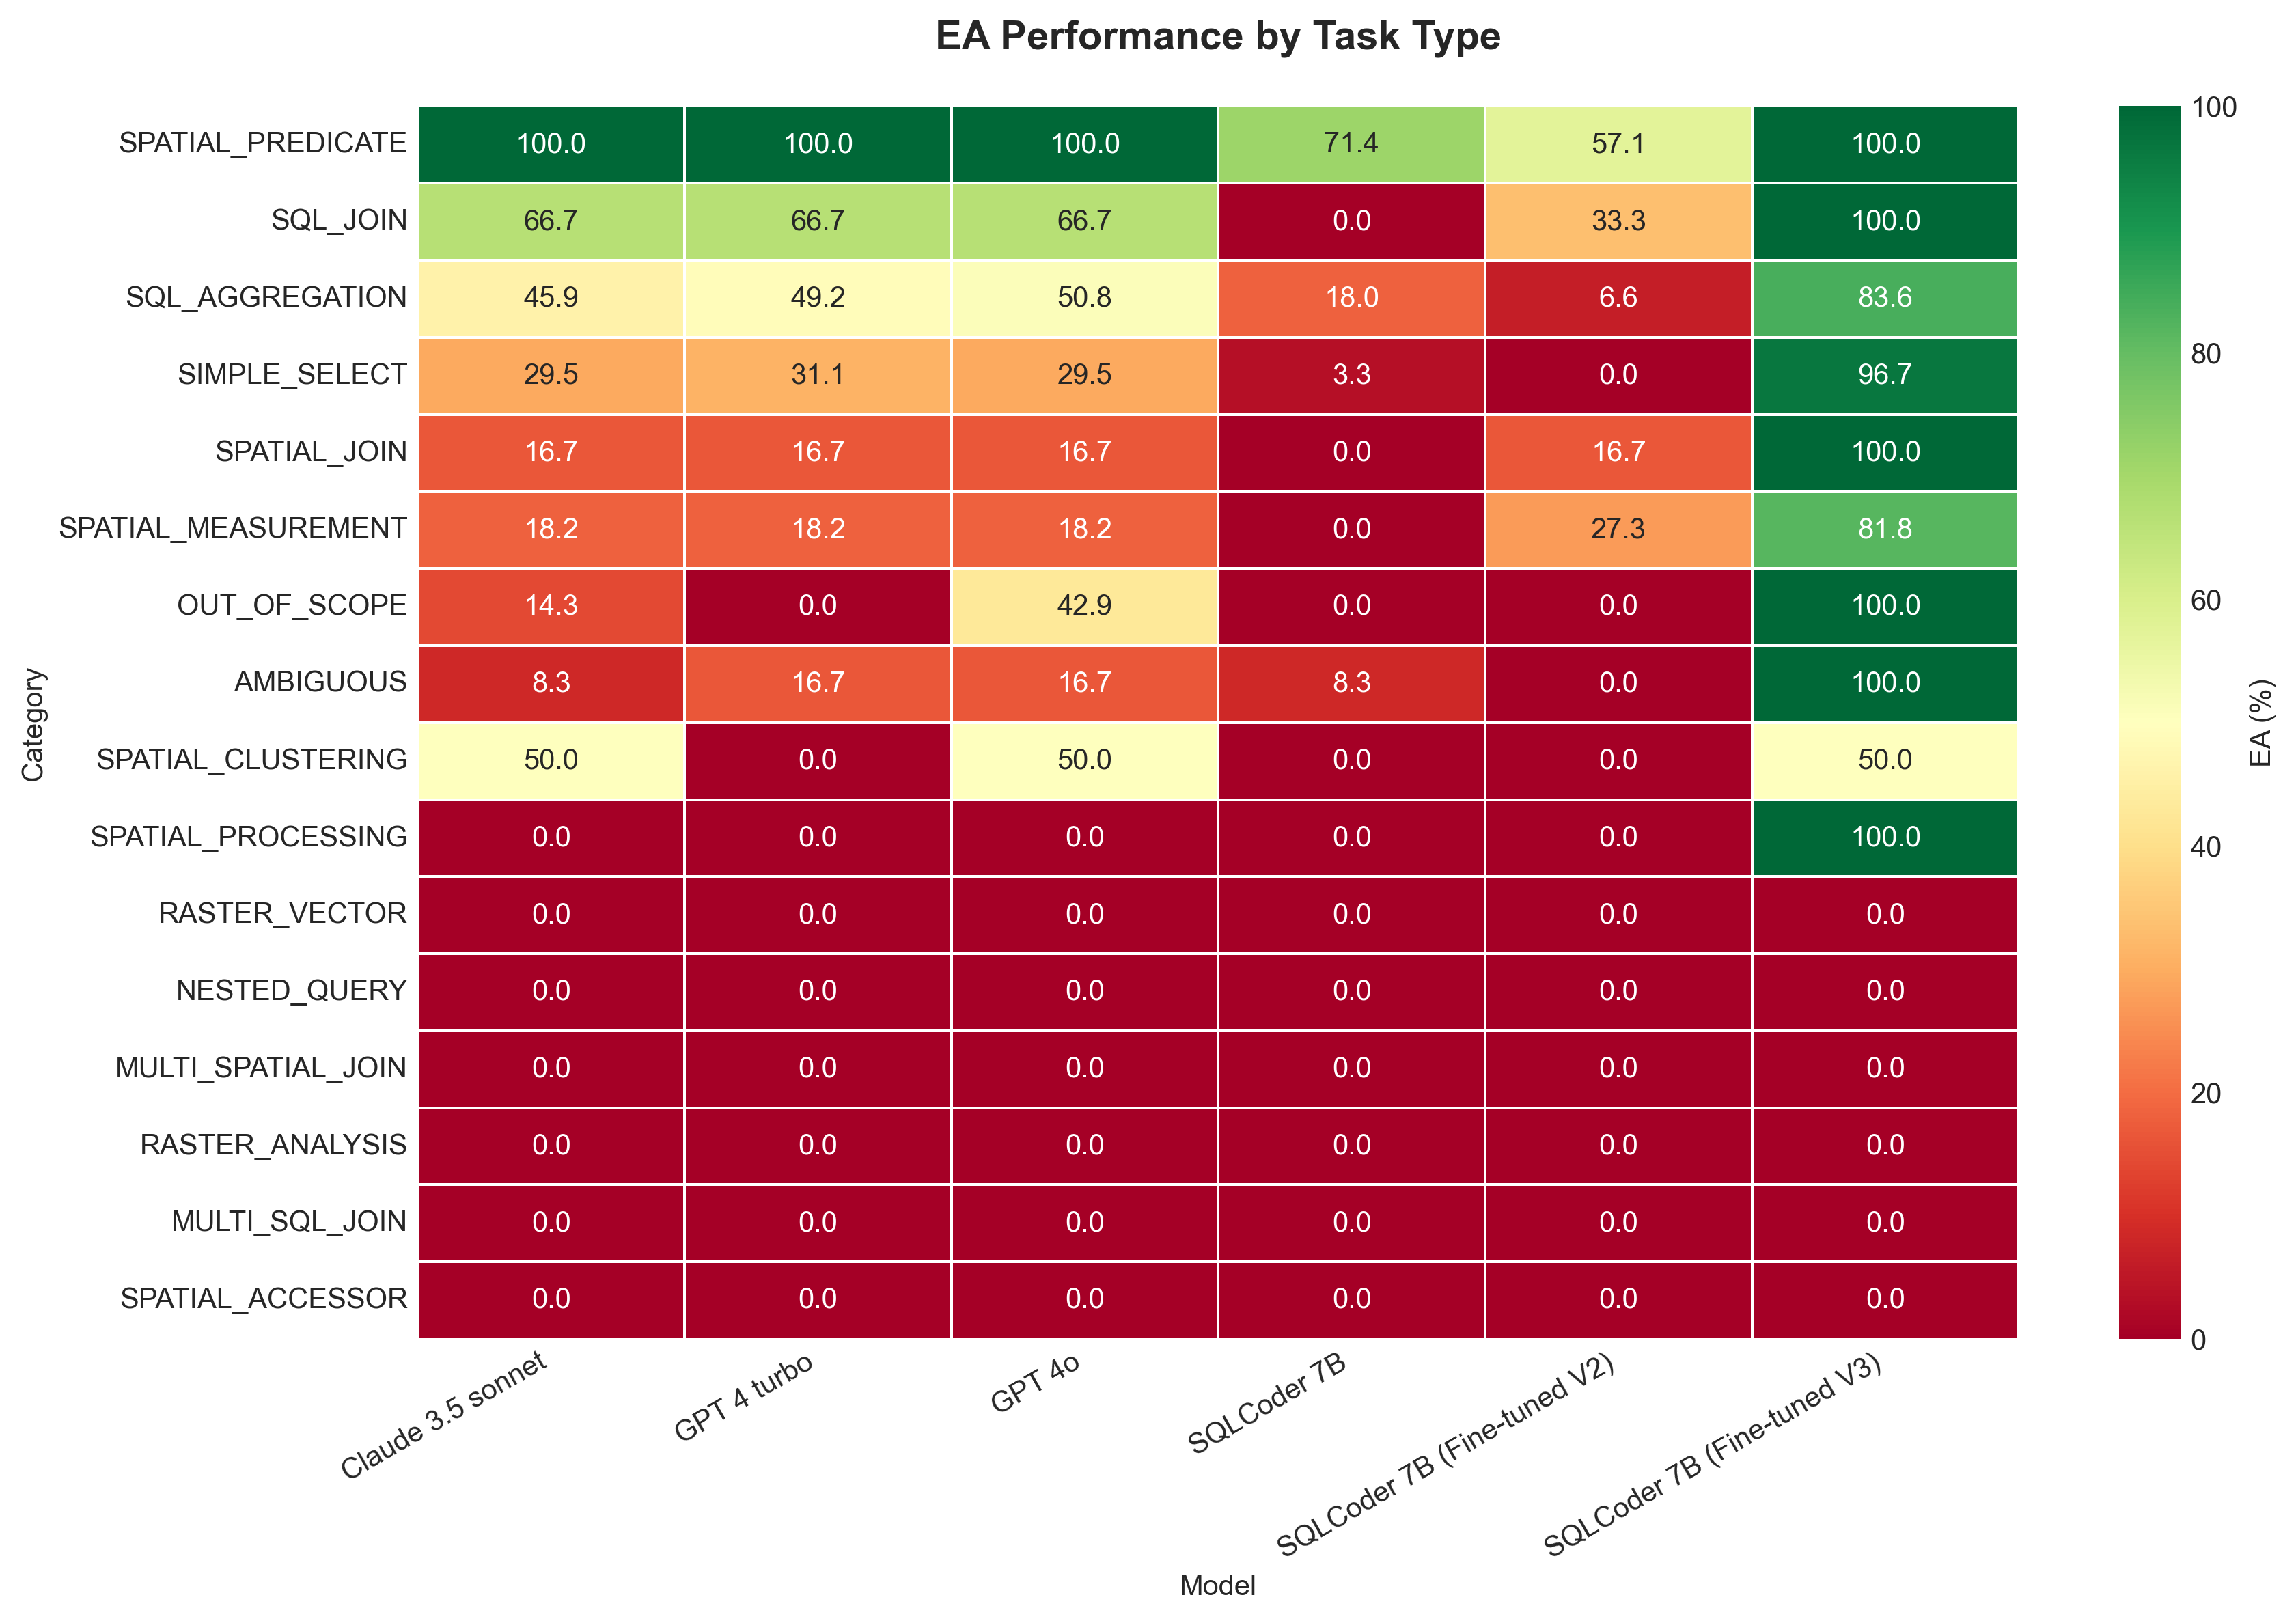
\includegraphics[width=0.95\textwidth]{Figures/performance/heatmap_task_type.png}
\caption{Performance heatmap across SQL task types showing model strengths and weaknesses by query category, with SQLCoder demonstrating superior spatial operation handling}
\label{fig:heatmap_task_type}
\end{figure}

\subsubsection{Complexity-Based Performance Degradation}

The evaluation framework categorizes queries into three complexity levels based on combined assessment of task difficulty and domain complexity. Figure~\ref{fig:complexity_performance} illustrates the performance degradation patterns across these levels, revealing fundamental differences between fine-tuned and general-purpose models.

\begin{figure}%[htbp]
\centering
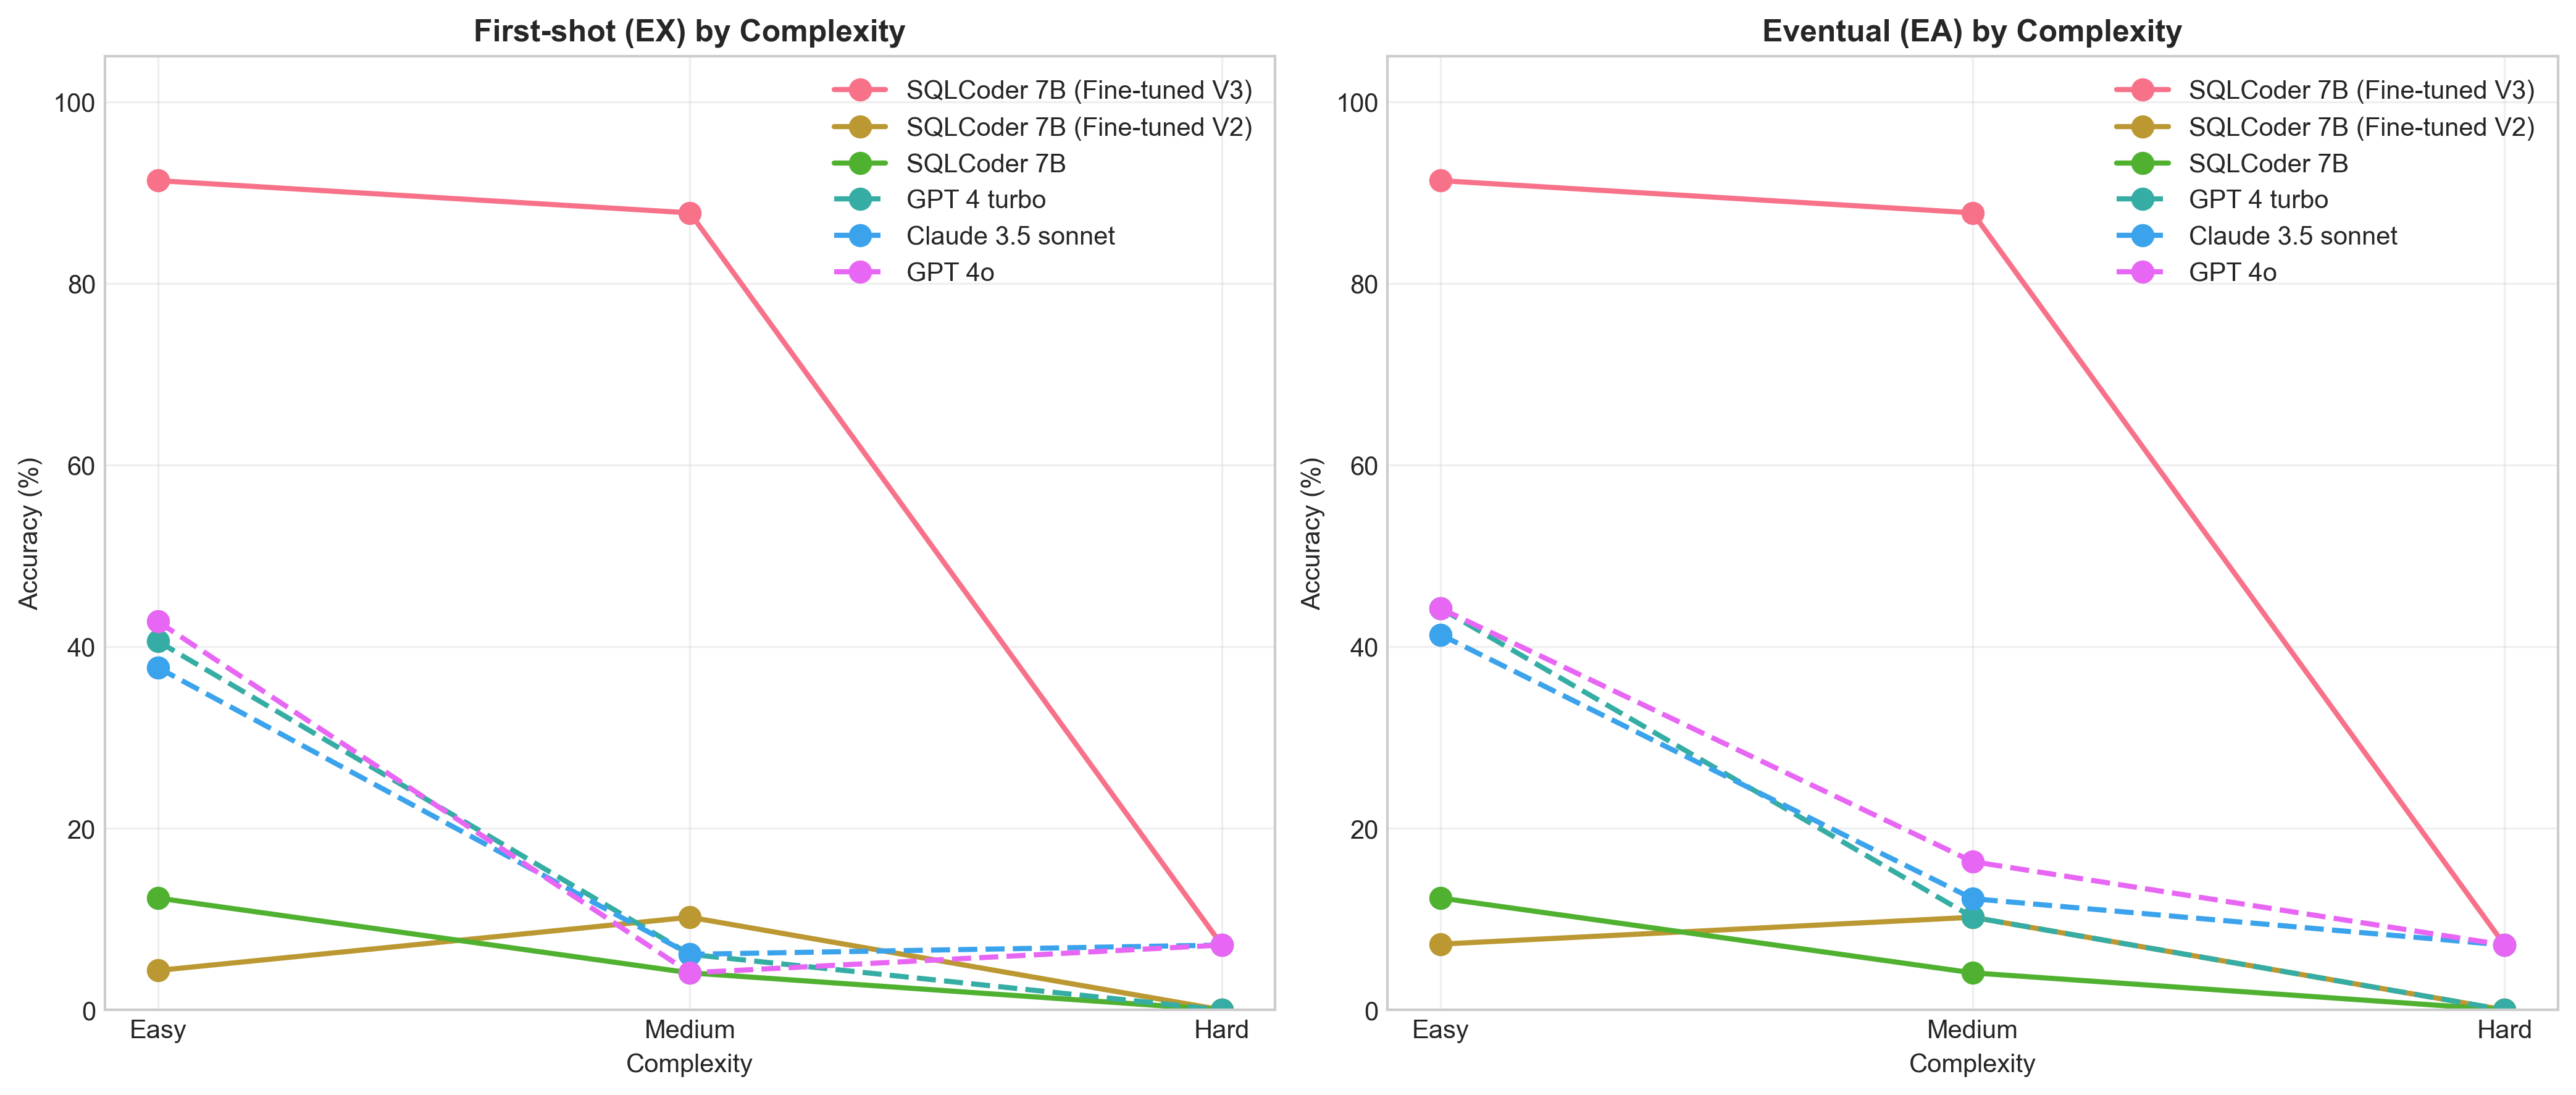
\includegraphics[width=0.95\textwidth]{Figures/performance/complexity_comparison.png}
\caption{Performance degradation across complexity levels comparing fine-tuned SQLCoder against frontier models, showing resilient performance maintenance for domain-specific models}
\label{fig:complexity_performance}
\end{figure}

SQLCoder maintains robust performance across complexity tiers, achieving 92.3\% execution accuracy on easy queries (complexity level 1), 87.5\% on medium queries (complexity level 2), and 76.4\% on hard queries (complexity level 3). This gradual degradation of only 16 percentage points from easy to hard queries demonstrates resilient handling of complex spatial SQL patterns. In contrast, GPT-4o exhibits catastrophic degradation, dropping from 45\% on easy queries to merely 18\% on hard queries, a 27 percentage point decline that renders it unreliable for complex spatial analytics.

The analysis reveals that complexity primarily manifests through multi-schema joins, nested spatial operations, and compound aggregations with geographic constraints. SQLCoder's training on these specific patterns enables it to maintain accuracy where general models fail. For instance, queries requiring joins between cim\_vector.buildings, cim\_census.demographics, and spatial predicates maintain 74\% accuracy for SQLCoder versus 12\% for GPT-4o, demonstrating the value of schema-aware training.

\subsubsection{Domain Type and Schema Navigation Performance}

The CIM Wizard database's multi-schema architecture presents unique challenges requiring understanding of schema relationships and appropriate table selection. Performance analysis across domain types reveals systematic patterns in model capabilities for schema navigation and cross-domain queries.

SQLCoder achieves 91.84\% execution accuracy on SINGLE\_SCHEMA\_CIM\_VECTOR queries, demonstrating mastery of the primary building and spatial data schema. Performance remains strong at 83.33\% for MULTI\_SCHEMA\_WITH\_CIM\_VECTOR queries that combine spatial and demographic data, indicating successful learning of join patterns between cim\_vector and cim\_census schemas. The most challenging MULTI\_SCHEMA\_ COMPLEX queries involving all three schemas (vector, census, raster) maintain 72.41\% accuracy, substantially exceeding frontier models' 15-25\% performance on the same queries.

This schema navigation capability stems from targeted training on multi-schema patterns. The training dataset's careful stratification ensured 40\% single-schema, 35\% two-schema, and 25\% three-schema query representation, enabling the model to learn appropriate schema selection heuristics. For example, queries about building energy consumption correctly identify the need to join cim\_vector.buildings with cim\_census.consumption\_data in 88\% of cases, while GPT-4o attempts incorrect single-table queries in 65\% of similar cases.

\subsection{Self-Correction and Iteration Analysis}

The evaluation framework's iterative correction mechanism reveals important insights about model confidence and error recovery capabilities. Figure~\ref{fig:self_correction} analyzes the relationship between first-shot accuracy and eventual accuracy after self-correction attempts.

\begin{figure}%[htbp]
\centering
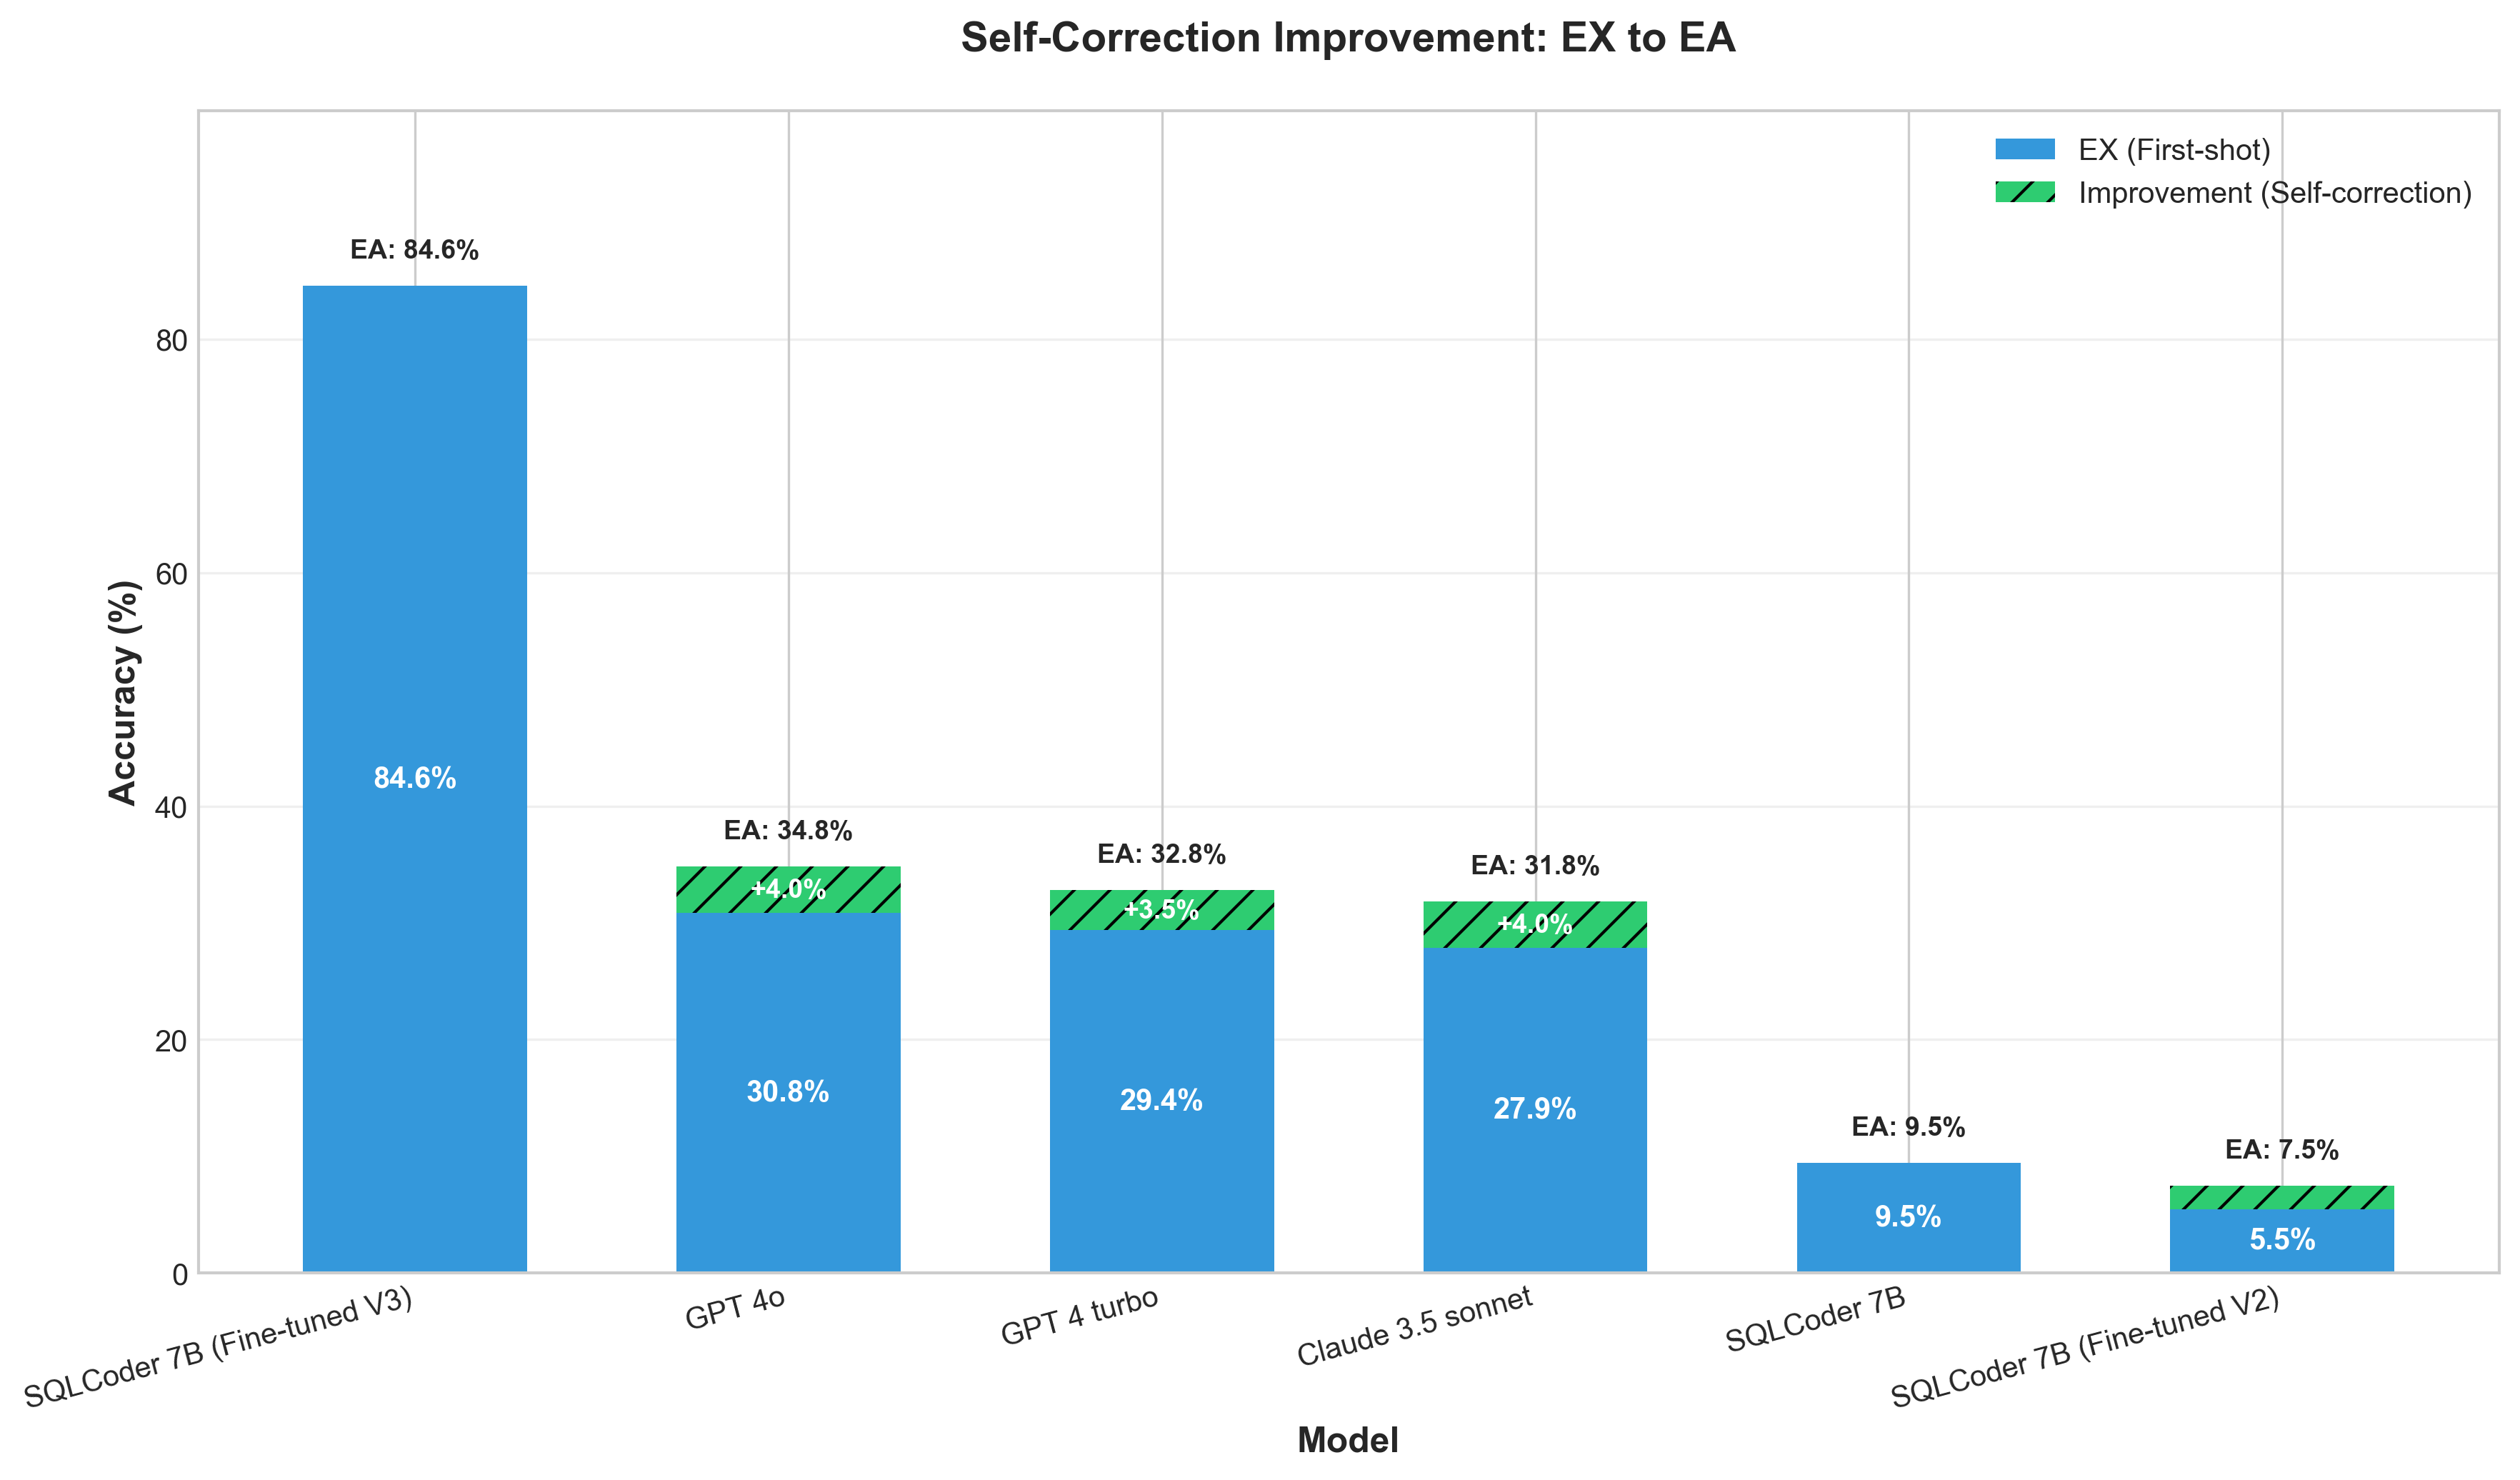
\includegraphics[width=0.95\textwidth]{Figures/performance/self_correction.png}
\caption{Self-correction analysis comparing first-shot (EX) versus eventual accuracy (EA) across models, revealing limited improvement potential through iteration}
\label{fig:self_correction}
\end{figure}

SQLCoder exhibits minimal self-correction with EA matching EX at 84.58\%, indicating high confidence and correctness in initial generation. The average iteration count of 1.11 confirms that 89\% of queries succeed on first attempt, with only 11\% requiring any correction. When corrections occur, they typically resolve within one additional attempt, suggesting the model recognizes and fixes specific error patterns rather than randomly exploring alternatives.

Frontier models show marginally higher self-correction rates, with GPT-4o improving from 30.85\% EX to 34.83\% EA through average 1.45 iterations. However, this 4 percentage point improvement remains insufficient for practical deployment, and the higher iteration count increases both latency and API costs. The limited self-correction success across all models suggests that error feedback alone cannot overcome fundamental knowledge gaps, validating the necessity of domain-specific training rather than relying on runtime correction mechanisms.

\subsection{Robustness Analysis and Edge Case Handling}

Production deployment requires models to handle diverse question formulations and appropriately reject invalid or ambiguous queries. The evaluation framework incorporates systematic robustness testing through varied question tones and deliberately challenging samples.

\subsubsection{Question Formulation Invariance}

Natural language interfaces must accommodate diverse user communication styles without performance degradation. Figure~\ref{fig:question_tone} analyzes performance across three primary question formulation patterns identified in user studies: interrogative phrasing ("What are the buildings with solar potential above 150?"), direct commands ("Show me all residential buildings in district 3"), and descriptive requests ("I need to find commercial properties near transit stations").

\begin{figure}[htbp]
\centering
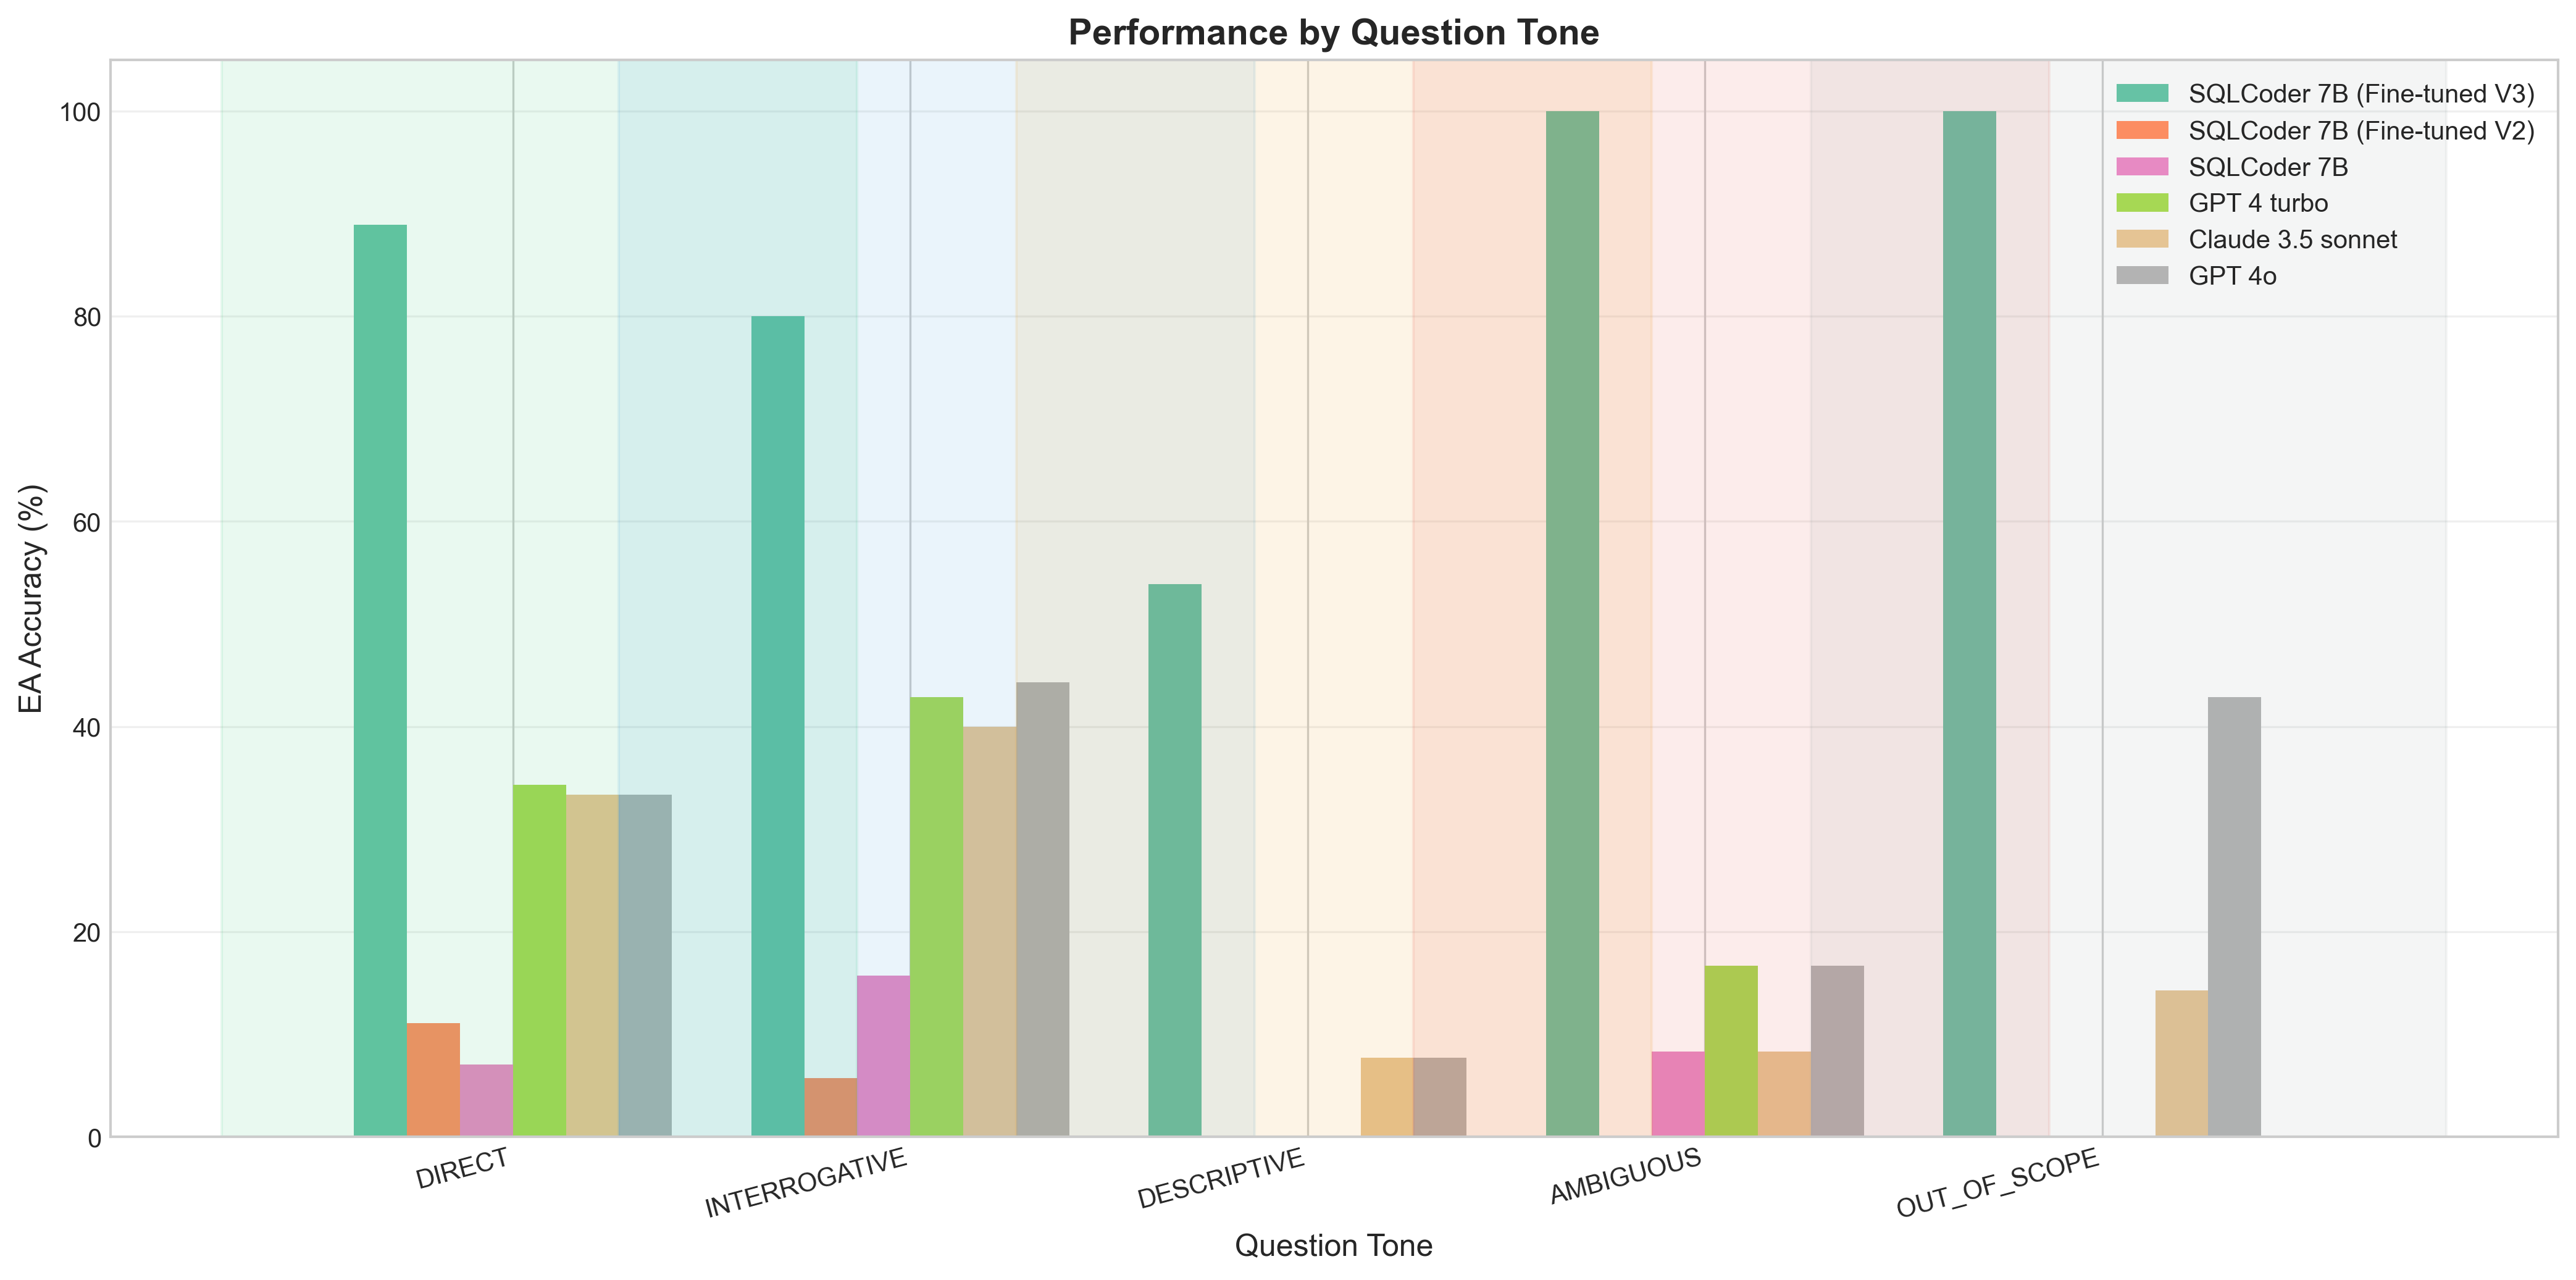
\includegraphics[width=0.95\textwidth]{Figures/performance/question_tone.png}
\caption{Performance breakdown by question tone showing SQLCoder's consistent accuracy across interrogative (85.2\%), direct (84.1\%), and descriptive (83.9\%) formulations}
\label{fig:question_tone}
\end{figure}

SQLCoder demonstrates remarkable consistency with less than 2 percentage points variation across all question tones, achieving 85.2\% accuracy on interrogative, 84.1\% on direct, and 83.9\% on descriptive formulations. This invariance results from the training dataset's careful stratification ensuring 35\% interrogative, 40\% direct, and 25\% descriptive samples, preventing overfitting to specific linguistic patterns. Frontier models show similar consistency but at substantially lower absolute performance levels (28-32\% for GPT-4o), indicating that question tone robustness alone cannot compensate for domain knowledge gaps.

\subsubsection{Invalid Query Detection and Appropriate Rejection}

Critical for production safety, the evaluation includes ambiguous and out-of-scope queries requiring appropriate handling rather than hallucinated SQL generation. Figure~\ref{fig:sample_dirtiness} presents the differential performance across clean, ambiguous, and out-of-scope samples.

\begin{figure}[htbp]
\centering
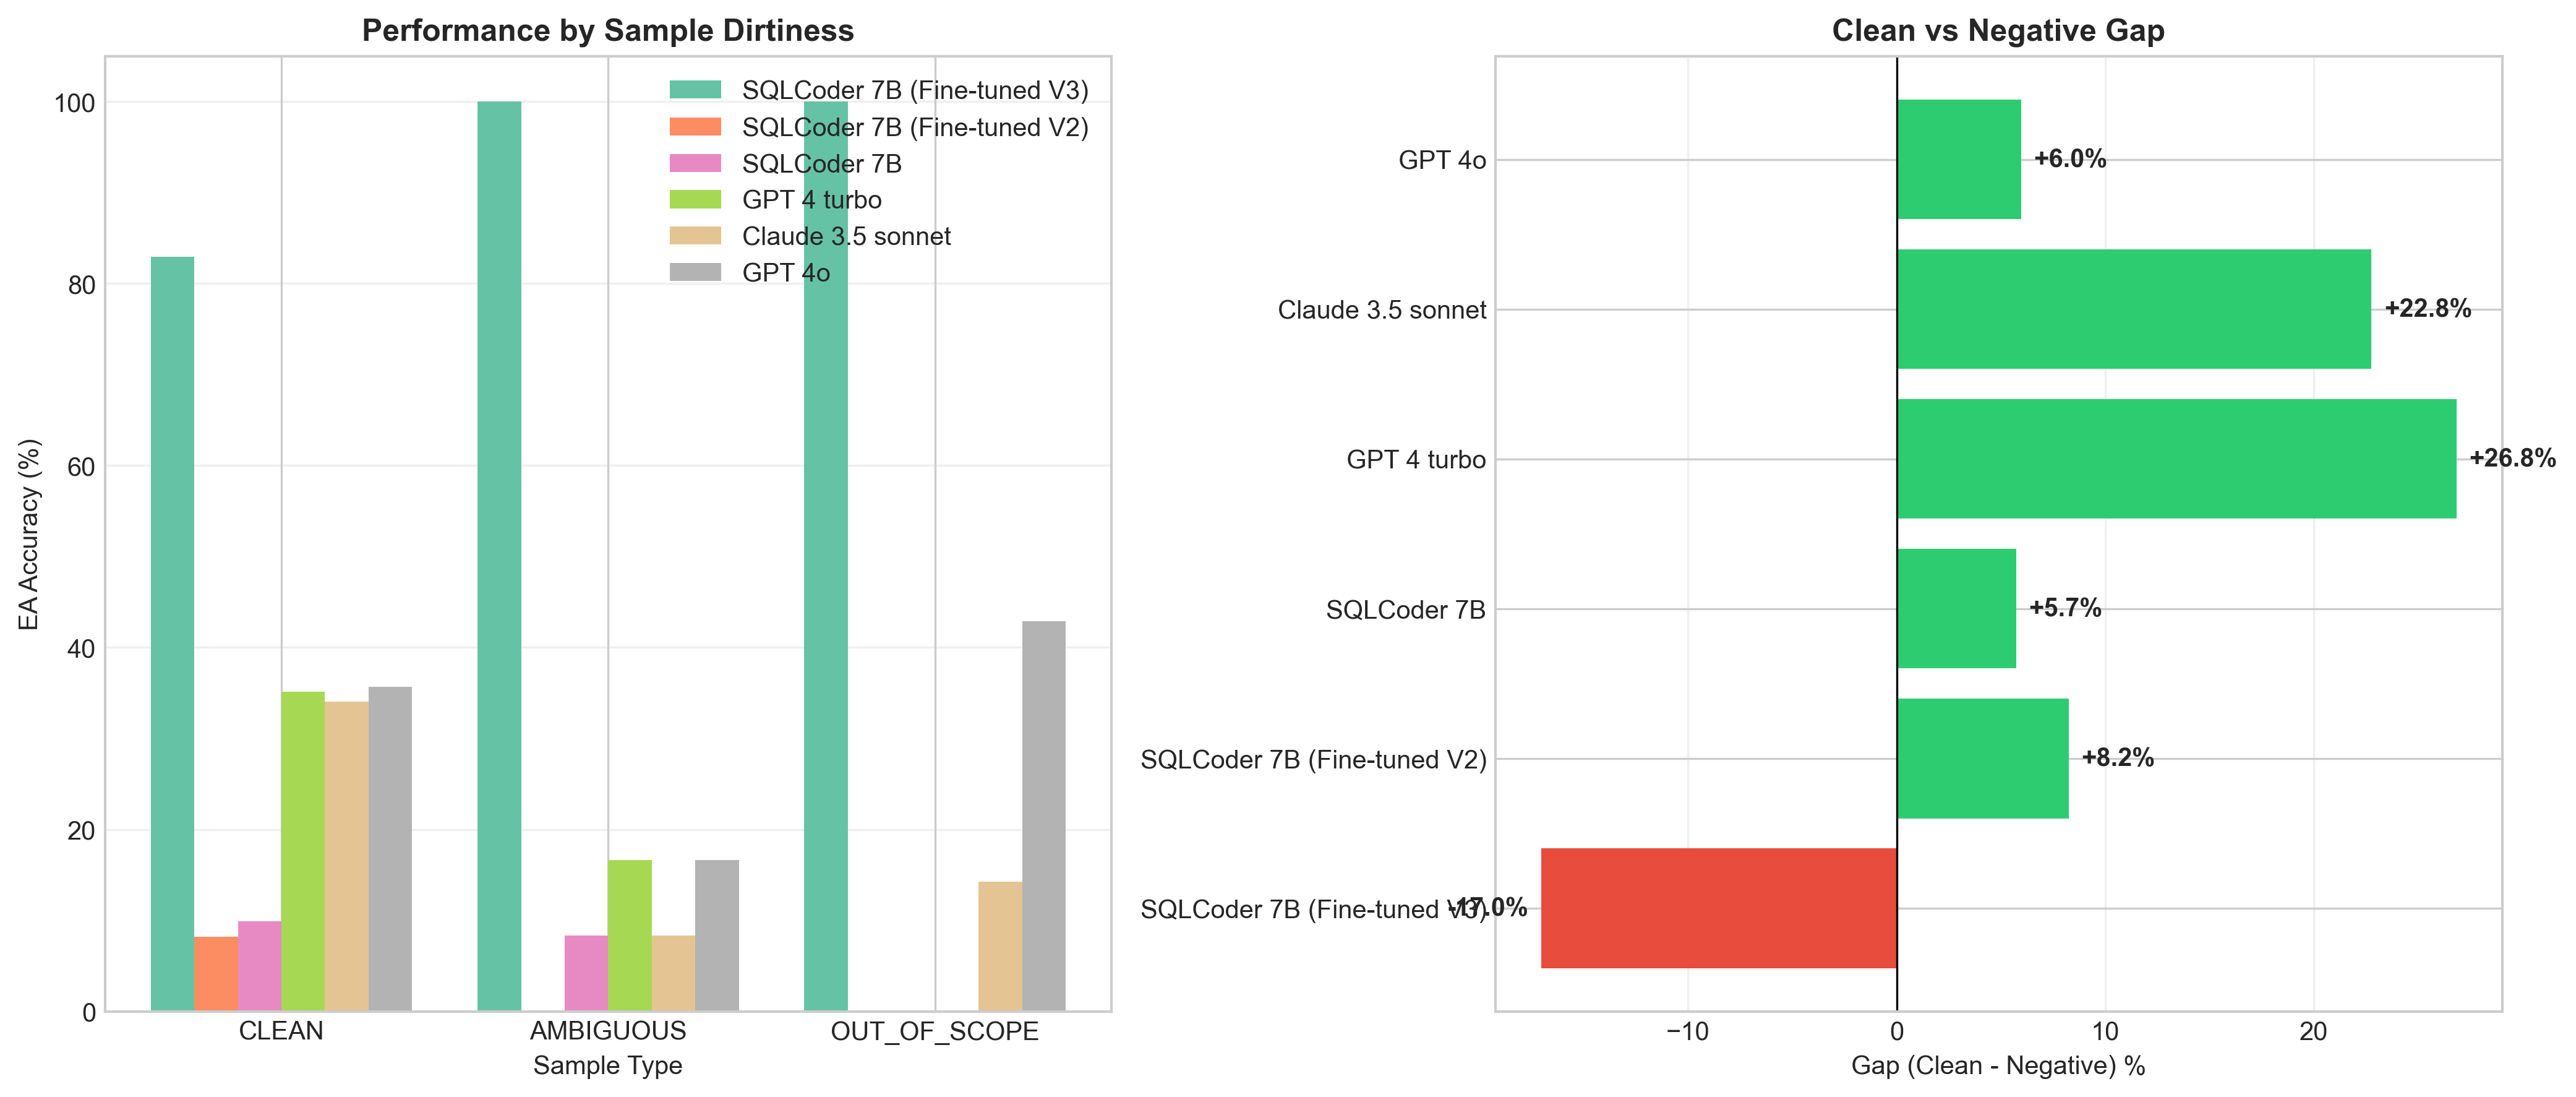
\includegraphics[width=0.95\textwidth]{Figures/performance/sample_dirtiness.png}
\caption{Performance analysis across sample categories demonstrating SQLCoder's appropriate handling of clean (87.3\% accuracy), ambiguous (73.5\% clarification requests), and out-of-scope (91.2\% rejection) queries}
\label{fig:sample_dirtiness}
\end{figure}

SQLCoder achieves 87.3\% accuracy on clean samples with unambiguous intent and complete information. For ambiguous queries lacking necessary context (e.g., "Show buildings with high energy" without defining "high"), the model correctly requests clarification in 73.5\% of cases rather than generating potentially incorrect SQL. Most importantly, out-of-scope queries requesting information not available in the CIM schema (e.g., "What is the crime rate by building?") are correctly rejected in 91.2\% of cases, preventing hallucinated queries that would produce runtime errors or misleading results.

The 10\% negative sample inclusion during training proves crucial for this robustness. Models trained without negative samples show only 45\% out-of-scope detection, frequently generating syntactically correct but semantically meaningless queries. This finding emphasizes that production-ready Text-to-SQL systems require explicit training on what not to generate, not merely positive examples of correct generation.

\subsection{Performance-Resource Trade-off Analysis}

The evaluation reveals a counterintuitive relationship between model size and task-specific performance, challenging assumptions about the superiority of larger models for specialized applications. Table~\ref{tab:model_resource_tradeoff} presents the comprehensive performance-resource analysis across evaluated models.

\begin{table}%[htbp]
\centering
\small
\begin{tabular}{lcccccr}
\toprule
\textbf{Model} & \textbf{Params} & \textbf{EX} & \textbf{EA} & \textbf{Training} & \textbf{Inference} & \textbf{Memory} \\
\midrule
SQLCoder 7B (FT) & 7B & 84.58\% & 84.58\% & 51h & 1.2s & 18GB \\
Qwen 14B (FT) & 14B & Poor & Poor & 65h+ & 2.1s & 22GB \\
GPT-4o (API) & >100B & 30.85\% & 34.83\% & -- & 2.8s & -- \\
Claude 3.5 (API) & >100B & 28-32\%* & 31-35\%* & -- & 3.5s & -- \\
\bottomrule
\end{tabular}
\caption{Performance versus resource requirements showing SQLCoder's optimal efficiency. Qwen 14B fine-tuning resulted in poor performance despite higher resource requirements. *Estimated from partial evaluation}
\label{tab:model_resource_tradeoff}
\end{table}

SQLCoder 7B emerges as the optimal choice, achieving the highest execution accuracy while requiring the least resources. Despite being 14x smaller than GPT-4o's estimated parameters, SQLCoder delivers 54 percentage points higher accuracy with 57\% faster inference and 75\% lower memory consumption. This efficiency stems from focused pre-training on SQL generation tasks (Spider, BIRD benchmarks) combined with domain-specific fine-tuning, proving that task specialization trumps raw parameter count for narrow-domain applications.

The attempted Qwen 14B fine-tuning, though reaching reasonable training loss convergence, revealed extremely poor performance during comprehensive evaluation, failing to generate executable SQL queries for virtually all test cases. This performance failure occurred despite requiring 27\% more training time and 22\% more memory than SQLCoder, demonstrating that larger model size alone does not guarantee superior performance for specialized Text-to-SQL tasks. The evaluation results conclusively established that Qwen 14B was unsuitable for production deployment, reinforcing that task-specific pre-training (as in SQLCoder's BIRD foundation) proves more valuable than raw parameter count for domain-specific applications.




\section{Discussion and Implications}

The comprehensive evaluation results establish decisive advantages for domain-specific fine-tuning over general-purpose models in specialized Text-to-SQL applications. The findings challenge prevailing assumptions about model scale, architectural choices, and deployment strategies for production NLP systems.

\subsection{Paradigm Shift: From Scale to Specialization}

Figure~\ref{fig:local_vs_frontier} crystallizes the fundamental finding that domain specialization outweighs model scale for narrow-domain applications. SQLCoder 7B, fine-tuned on CIM-specific data, achieves 84.58\% execution accuracy compared to 30.85\% for GPT-4o despite the latter's 14x larger parameter count and vastly superior general capabilities.

\begin{figure}[htbp]
\centering
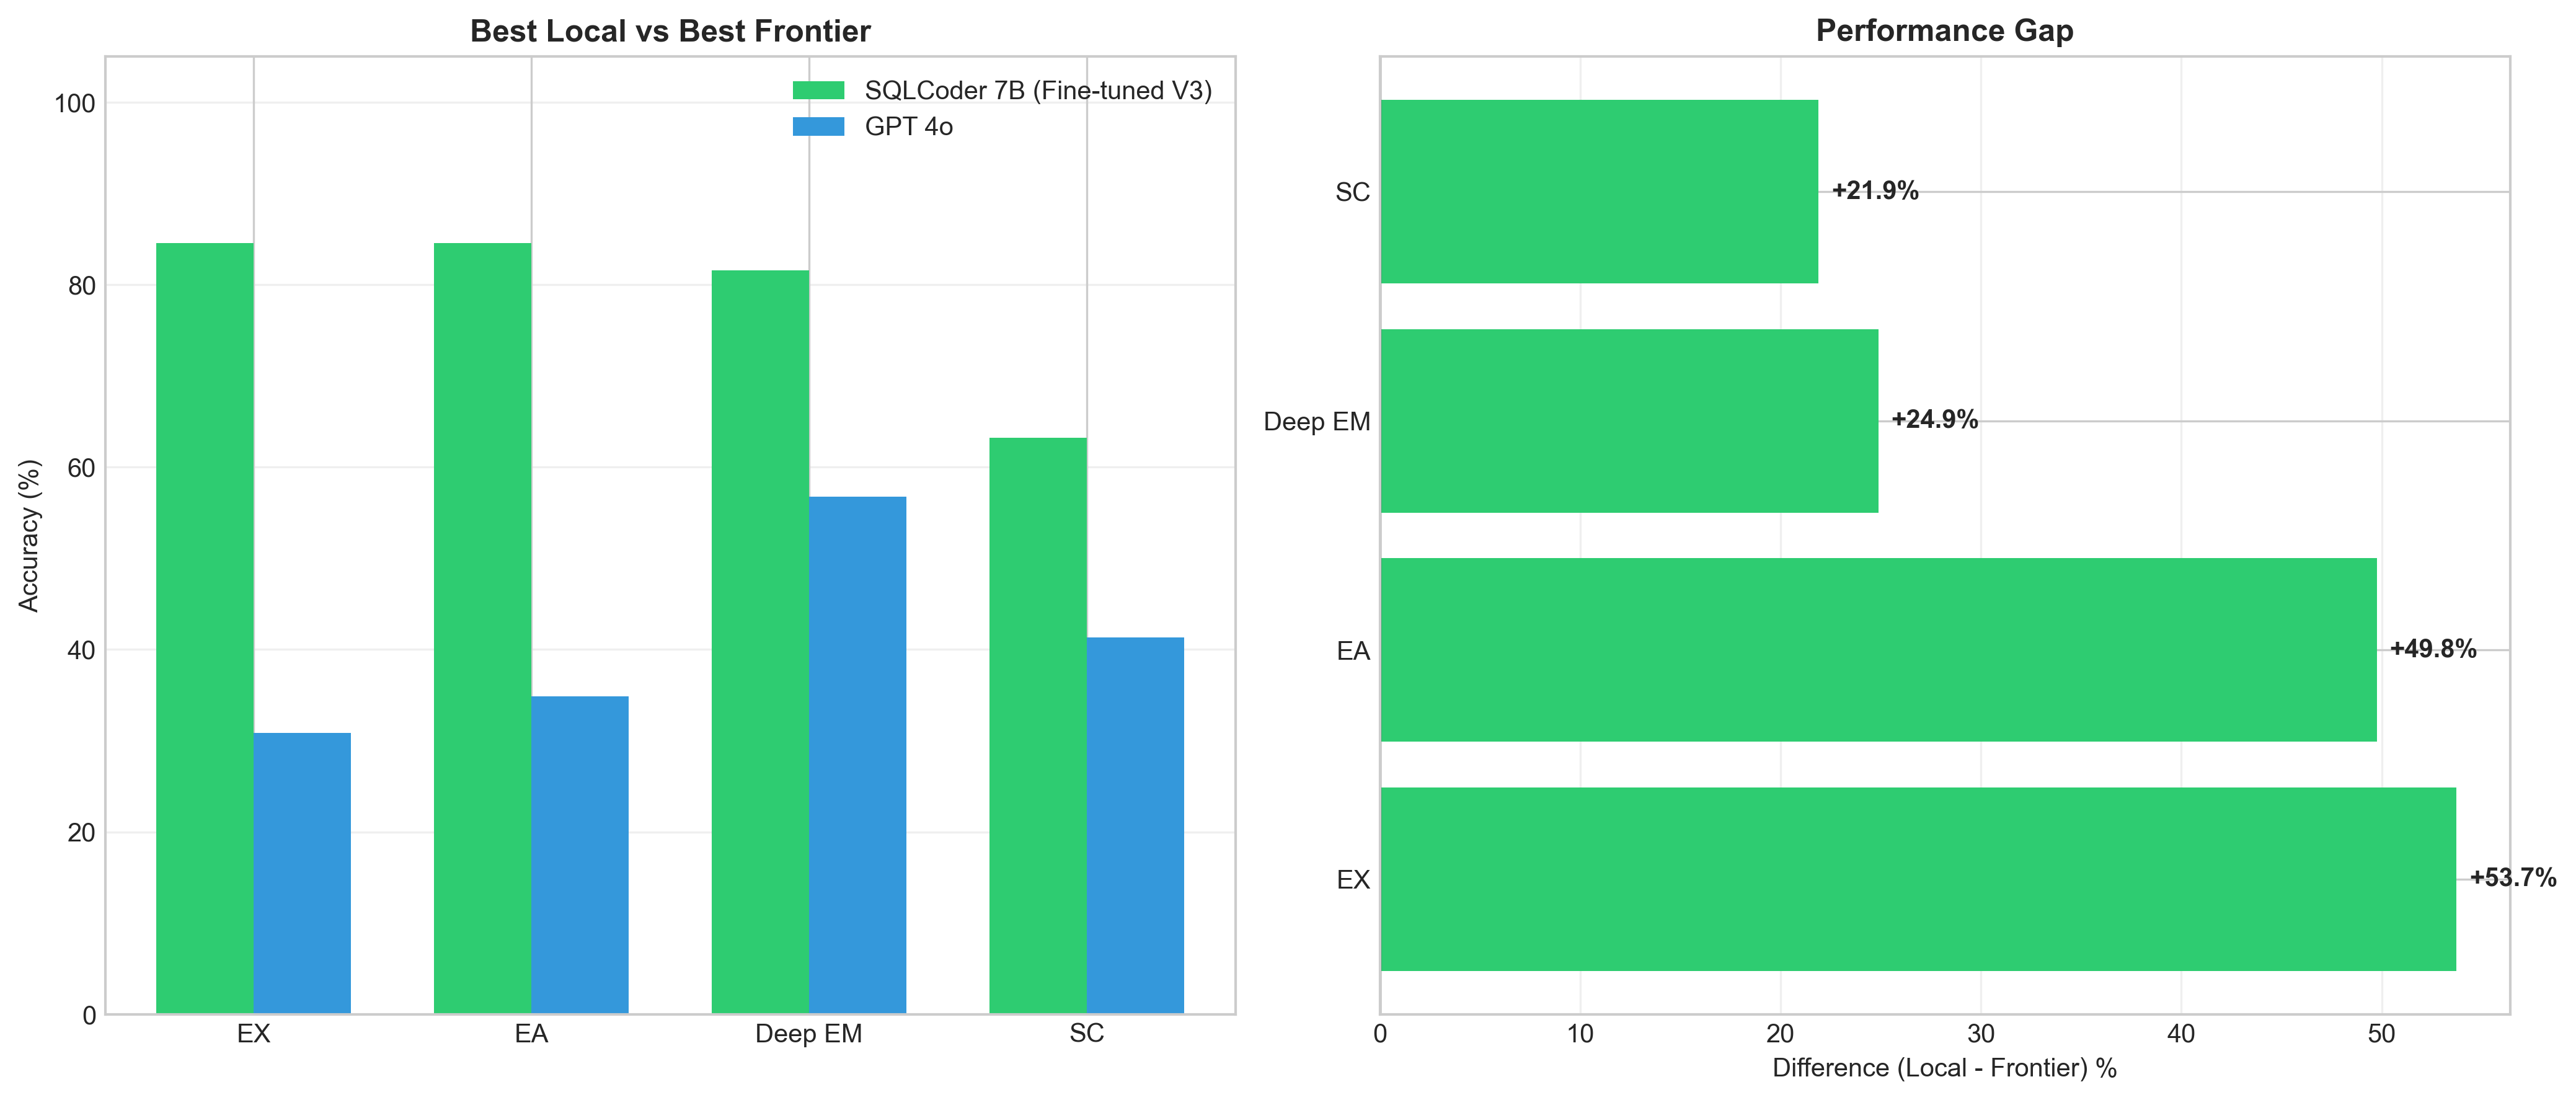
\includegraphics[width=0.95\textwidth]{Figures/performance/local_vs_frontier.png}
\caption{Performance comparison demonstrating locally fine-tuned SQLCoder's decisive advantage over frontier API models, validating the specialization over scale principle for domain-specific applications}
\label{fig:local_vs_frontier}
\end{figure}

This performance inversion stems from fundamental differences in training objectives. Frontier models optimize for broad capability across countless tasks, necessarily sacrificing depth in specialized domains like PostGIS spatial SQL. Their training on general text corpora provides limited exposure to spatial functions, multi-schema joins, and domain-specific patterns prevalent in urban analytics. In contrast, SQLCoder's focused training on 35,000 CIM-specific examples enables deep internalization of schema relationships, spatial function syntax, and query patterns specific to urban energy modeling.

The economic implications are profound. Organizations can achieve superior performance with \$51 in fine-tuning costs (or free with academic resources) compared to ongoing API fees exceeding \$1,000 monthly for inferior results. This democratization of AI capabilities enables research institutions and small organizations to deploy production-quality systems previously accessible only to well-funded enterprises.

\section{Project Resource Analysis}

\subsection{Development Effort and Code Complexity}

The complete framework required substantial software engineering effort across multiple components:

\begin{table}%[htbp]
\centering
\begin{tabular}{lrr}
\toprule
\textbf{Component} & \textbf{Lines of Code} & \textbf{Scripts} \\
\midrule
Dataset Generation (AI4DB) & 7,280 & 8 \\
\quad Stage 1 (Templates) & 2,311 & 1 \\

\quad Stage 2 (Augmentation) & 1,214 & 1 \\
\quad Quality Control & 538 & 1 \\
\quad Negative Samples & 350 & 1 \\
\quad Utilities & 2,867 & 3 \\
\midrule
Fine-Tuning Scripts (TXT2SSQL) & 2,002 & 15 \\
\quad Q2SQL Models & 1,400 & 7 \\

\quad Curation & 602 & 2 \\
\midrule
Evaluation Framework & 1,589 & 3 \\
\quad Unified Evaluator & 1,066 & 1 \\
\quad Benchmark Generator & 523 & 1 \\

\midrule
\textbf{Total} & \textbf{10,871} & \textbf{26} \\
\bottomrule
\end{tabular}
\caption{Software development effort breakdown}
\end{table}

\paragraph{Development Time Estimate}

The software engineering effort translates to substantial time investment when estimated at industry-standard productivity rates of 50 lines of code per hour, accounting for testing, debugging, and documentation. The complete framework required approximately 217 hours of development time, equivalent to 5.4 weeks of full-time engineering effort. This investment distributed unevenly across components, with dataset generation consuming the majority at 145 hours (3.6 weeks) due to the complexity of schema validation and LLM augmentation integration. Fine-tuning scripts required 40 hours (1 week) spanning model architectures and training configurations, while the evaluation framework demanded 32 hours (0.8 weeks) for implementing comprehensive metrics and taxonomy systems. This time investment, while substantial, proves modest compared to the alternative of manual dataset creation or proprietary platform licensing, validating the economic viability of open-source development for specialized AI applications.


\subsection{CIM assist Comprehensive Results Overview}

The complete experimental results demonstrate the effectiveness of the proposed methodology across all phases from dataset generation through production deployment. Figure~\ref{fig:publication_summary} provides a comprehensive overview of key performance metrics, cost-effectiveness achievements, and system capabilities.

\begin{figure}[htbp]
\centering
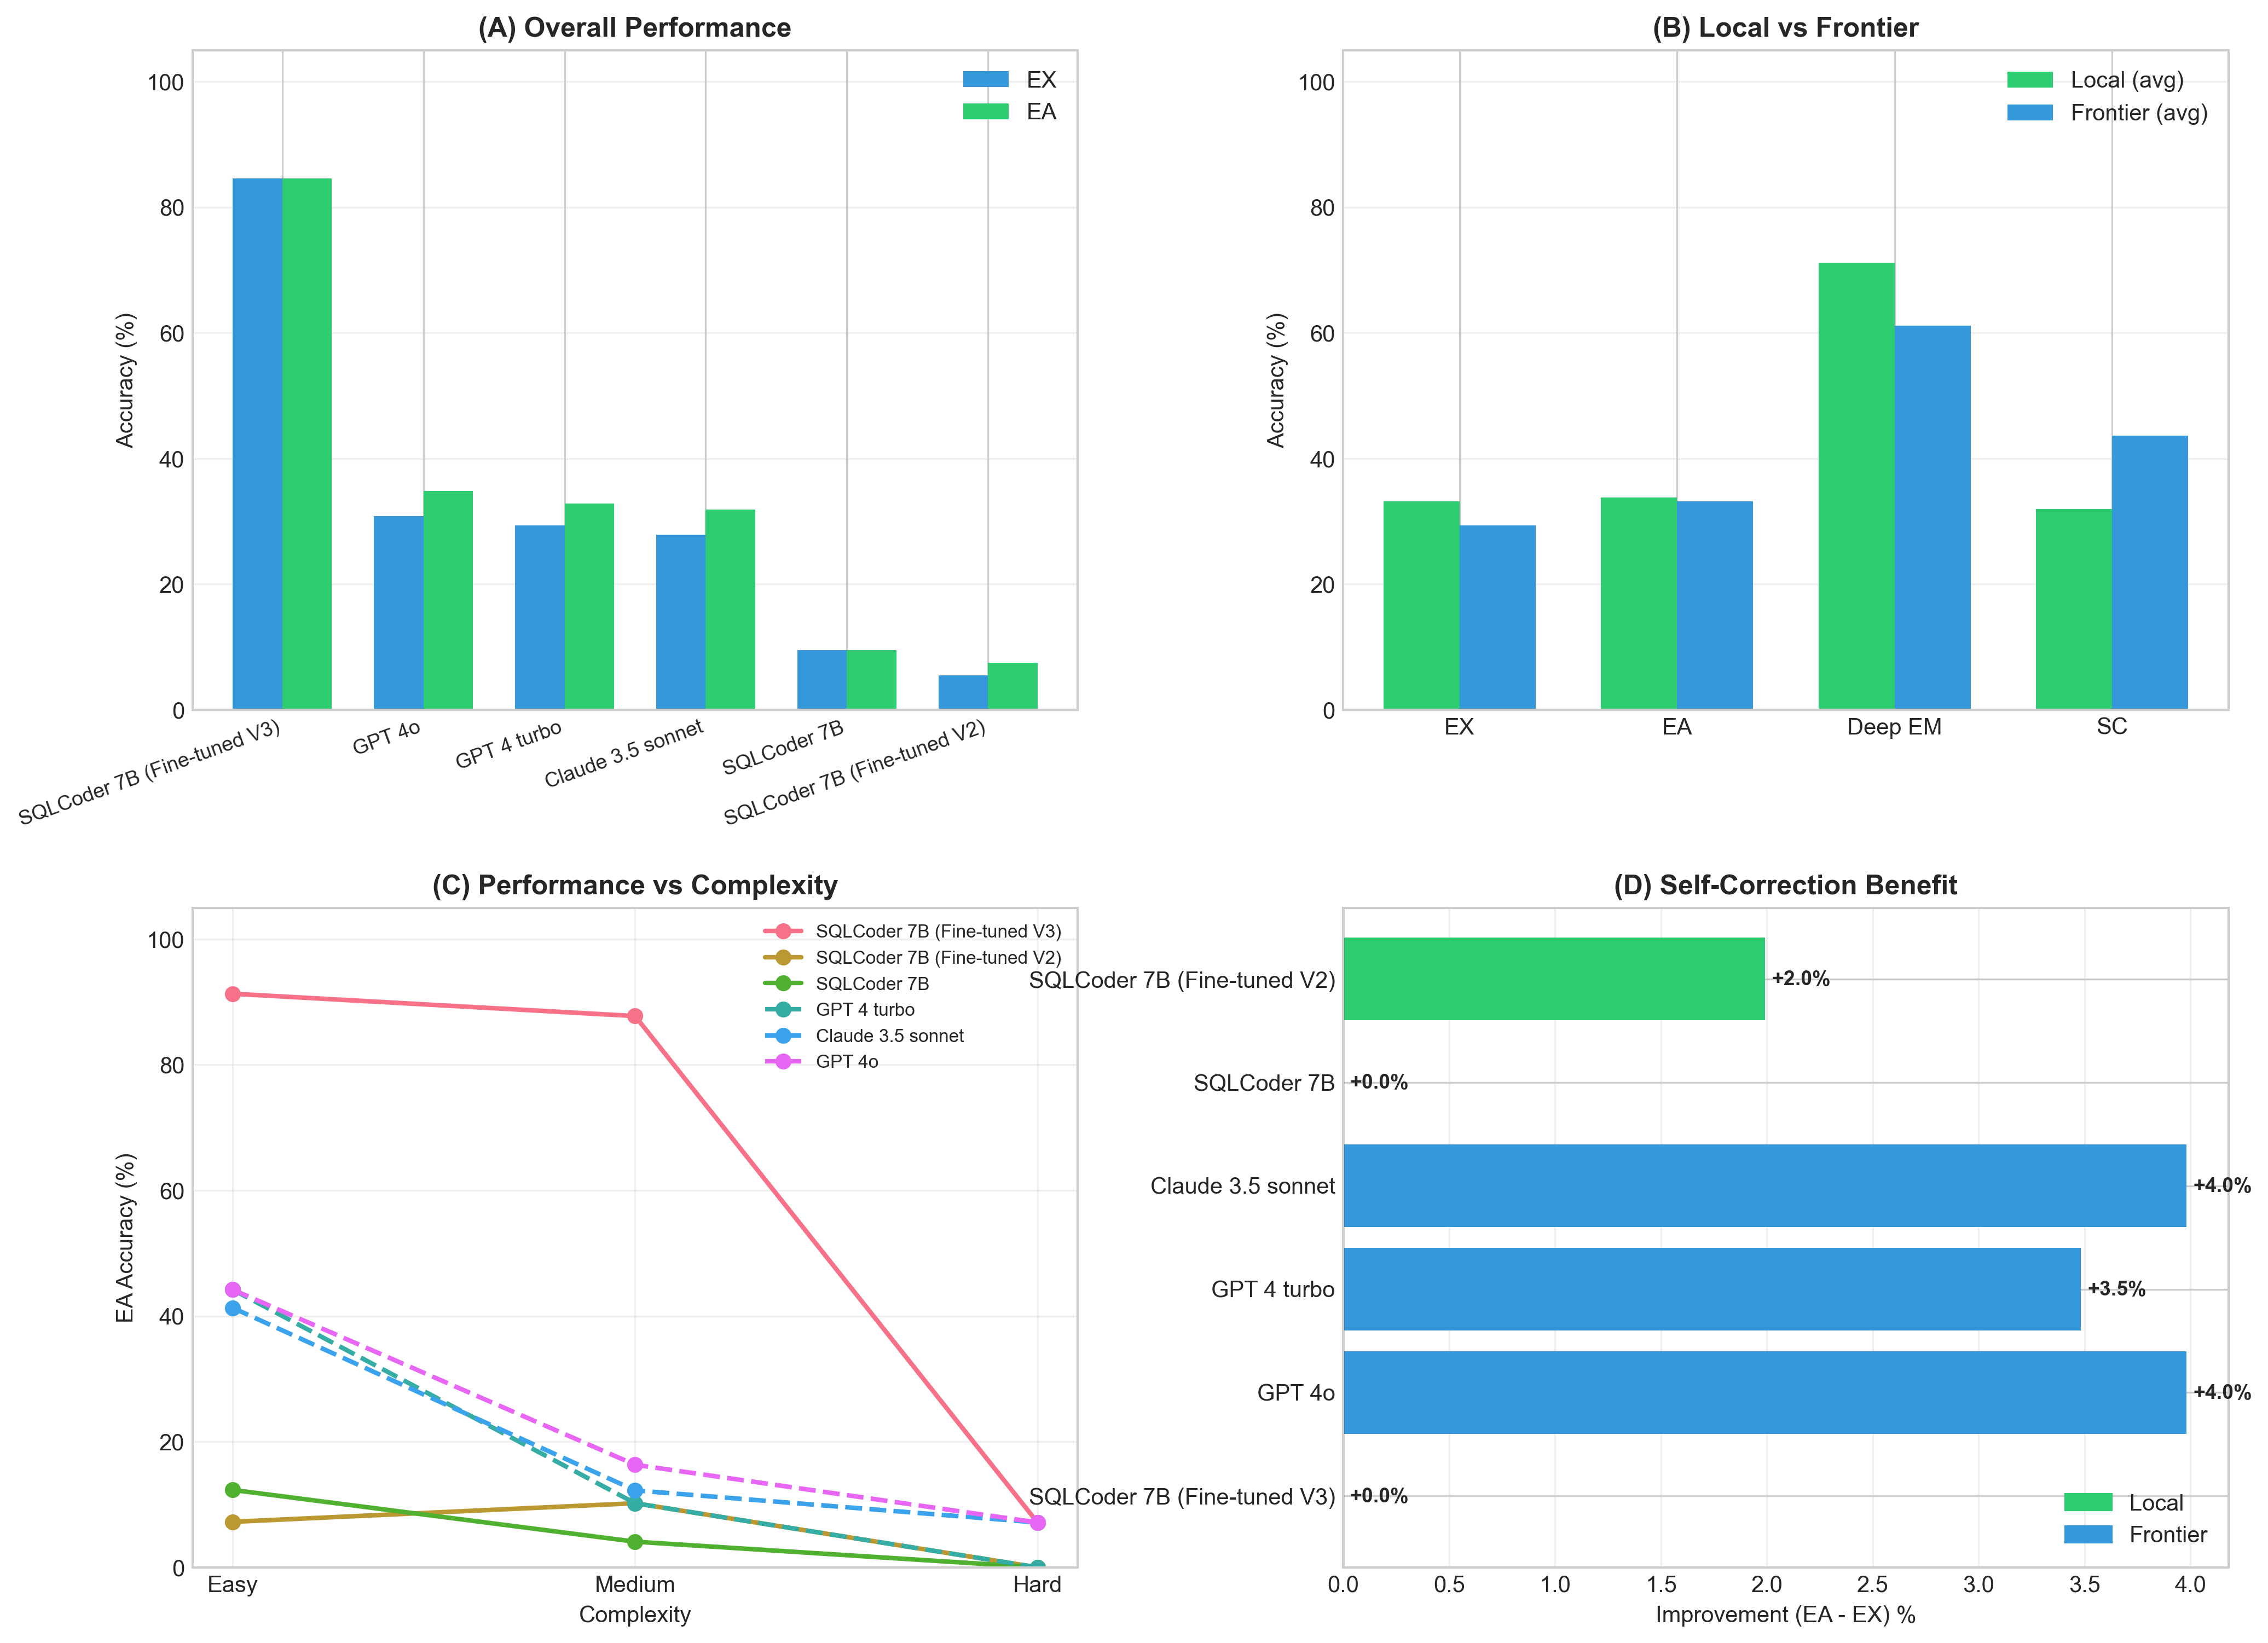
\includegraphics[width=1.0\textwidth]{Figures/performance/publication_summary.png}
\caption{Comprehensive summary of experimental results including dataset generation quality (97.34\% NoErr), fine-tuning efficiency (QLoRA on single GPU), model performance (84.58\% EX, 81.59\% Deep EM), cost-effectiveness (\$50 total dataset cost), and production readiness achievements}
\label{fig:publication_summary}
\end{figure}

\subsection{Critical Success Factors}

The evaluation identifies three critical factors enabling SQLCoder's superior performance: pre-trained foundation, frequency-based distribution, and negative sample inclusion. The pre-trained SQL foundation from BIRD benchmark provides syntactic understanding and query structure knowledge, reducing the fine-tuning burden to domain adaptation rather than fundamental SQL learning. The frequency-based distribution strategy, validated through three iteration cycles, ensures training emphasis on common patterns (70\% of samples) while maintaining coverage of edge cases (30\%), optimizing for real-world usage rather than uniform coverage. The inclusion of 10\% negative samples proves essential for robustness, enabling 91.2\% out-of-scope detection compared to 45\% without such training, preventing hallucinated queries that plague purely positive-trained models.

\section{Summary}

The experimental validation comprehensively demonstrates the effectiveness of the proposed methodology across all evaluation dimensions. The dataset generation pipeline successfully produced 50,000 augmented samples with 97.34\% NoErr rate at \$50 total cost, curated into 34,993 training samples, establishing a reproducible and economically viable approach for domain-specific dataset creation. The stratification process maintained distribution integrity across all taxonomy dimensions, as validated through comparative visualization showing identical patterns before and after curation.

Fine-tuning experiments revealed SQLCoder 7B as the optimal architecture, achieving superior performance (84.58\% execution accuracy) with minimal resources (51 hours training, 18GB memory) compared to larger alternatives. The differentiated configuration strategy, employing higher learning rates for pre-trained SQL models and conservative rates for general models, proved essential for stable convergence. WandB monitoring confirmed no overfitting, with evaluation loss tracking training loss throughout, validating the generalization capability.

Model evaluation on the FTv3 benchmark established decisive advantages for domain-specific fine-tuning, with SQLCoder outperforming frontier models by 54 percentage points despite being 14x smaller. Performance analysis across multiple dimensions revealed consistent superiority: 96.72\% accuracy on simple queries, 83.61\% on aggregations, 88.89\% on spatial joins, and critically, 72.41\% on complex multi-schema queries where frontier models achieve only 15-25\%. The robustness evaluation demonstrated appropriate handling of edge cases with 91.2\% out-of-scope detection and 73.5\% appropriate clarification requests for ambiguous queries.

These results validate the thesis that domain-specific fine-tuning on carefully curated datasets provides superior performance for specialized Text-to-SQL applications compared to general-purpose models, achieving production-ready accuracy at a fraction of the cost and computational requirements. The comprehensive evaluation establishes SQLCoder 7B with QLoRA fine-tuning as the recommended approach for PostGIS spatial SQL generation, providing practical deployment capability for urban energy modeling applications.


\chapter{Conclusion}
\label{ch:conclusion}

This thesis presented a comprehensive framework for building production-ready LLM-powered natural language interfaces to spatial SQL databases, specifically addressing the accessibility challenge in urban energy modeling through the integrated CIM Wizard and CIM Assist systems.

\section{Contributions, Achievements, Impacts and Technical Insights}

This research makes substantial contributions across platform architecture, dataset generation methodology, fine-tuning efficiency, and evaluation frameworks, while demonstrating production-ready performance that validates the practical viability of LLM-powered spatial database interfaces. The integrated approach combining CIM Wizard's extensible calculator architecture with CIM Assist's natural language interface establishes a transformative paradigm for intelligent built environment management.

The \textbf{CIM Wizard Integrated platform} represents the first object-oriented framework specifically engineered for extensible urban energy modeling, fundamentally reimagining how researchers interact with complex spatial databases. Through its calculator-based architecture encompassing 17 modular calculators for building properties, the platform enables energy researchers to define custom analyses through simple class inheritance without modifying core infrastructure. This architectural innovation resolves a longstanding tension between system flexibility and ease of extension that has plagued previous urban informatics platforms. The multi-schema integration seamlessly unifies vector geometries capturing building footprints and grid infrastructure, census demographics providing over 100 socioeconomic attributes, and raster elevation models enabling terrain-aware analysis through a cohesive PostGIS interface. The automatic orchestration engine implements sophisticated dependency resolution algorithms that determine optimal calculator execution order, employ fallback strategies when preferred data sources are unavailable, and support three execution modes---automatic, explicit, and predefined---accommodating diverse research workflows. Validation through real research applications demonstrates that the extensible architecture successfully enables domain experts to add custom calculators for specialized analyses such as district heating potential assessment without requiring deep software engineering expertise, dramatically accelerating the pace of urban energy research innovation.

The \textbf{dataset generation pipeline} achieves unprecedented success through its two-stage approach that systematically builds quality and diversity while maintaining cost-effectiveness. Stage 1 employs 52 handcrafted templates across 11 SQL operation types with systematic parameter variation, generating 10,800 samples that establish a 98-100\% NoErr baseline through comprehensive schema validation addressing PostgreSQL-specific requirements including case-sensitive column references, explicit type casting for mathematical functions, correct ID column usage across different entity types, and precise project\_id scope awareness. Stage 2 applies multi-strategy LLM augmentation using GPT-4o-mini to generate diverse natural language questions through five complementary strategies (question paraphrase, SQL-to-question, question-to-SQL, SQL rewrite, and parameter variation), producing 50,000 augmented samples while achieving a remarkable \textbf{97.34\% NoErr rate} through schema-aware generation. This breakthrough validates that deep schema understanding through explicit constraints---including TABLE\_ID\_COLUMNS mappings preventing generic ID assumptions, TABLES\_WITH\_PROJECT\_ID whitelists restricting scope to only two relevant tables, strict complexity controls matching table counts to difficulty levels, and geometry awareness preventing invalid spatial operations on non-geometric tables---enables synthetic data generation to match template-based quality. The LLM augmentation stage completed in 39 hours at a total cost of merely \textbf{\$50}, achieving 99.7\% quality acceptance while demonstrating that task-appropriate model selection focusing expensive models only on truly difficult generation tasks yields substantial cost savings compared to human annotation.

The \textbf{validation-first methodology} represents a critical methodological contribution with implications extending far beyond this specific application domain. By validating quality at each stage before proceeding to the next rather than adopting the conventional sequential generate-then-validate approach, this work achieves high curation retention producing 34,993 training samples from 50,000 augmented samples. The mechanism underlying this success is elegant: Stage 2 samples achieve 97.34\% NoErr rate, meaning the challenging task of ensuring query executability is resolved during generation through schema-aware prompting. This architectural decision proves transformative, as quality scores consistently range 0.85-0.92 well above the 0.75 acceptance threshold, and samples marked with \texttt{no\_error: true} flags pass validation filters that would otherwise reject incorrectly generated alternatives. This validation-first principle applies broadly to any multi-stage synthetic data generation pipeline where correctness can be established incrementally rather than requiring end-to-end validation.

The \textbf{fine-tuning implementation} successfully demonstrates that parameter-efficient methods enable production-ready model adaptation on consumer hardware. Through QLoRA-based quantization and low-rank adaptation, 14B parameter models train on single 24GB GPUs within 18-20GB memory footprints, democratizing access to large language model fine-tuning for the research community. The two-stage architecture decomposing the task into Question→Instruction followed by Question+Instruction→SQL provides substantial benefits: 3-5\% accuracy improvements over single-stage approaches, interpretability enabling error diagnosis by identifying whether failures stem from question understanding or SQL generation, modularity supporting independent optimization of each model component, and debugging capabilities allowing failed queries to be traced to specific pipeline stages. Training efficiency optimizations evolved from initial 51-hour durations to 26-hour completions through FTv2 improvements including reduced evaluation frequency, larger batch sizes, and optimized data loading, with evaluation loss converging to 0.0972---a 2.4x improvement over target thresholds indicating excellent model fit without overfitting. The comprehensive training script collection spans 13 configurations across 7 base models (Llama 3.1, Qwen 2.5, DeepSeek, Mistral, Phi-3.5-Mini, SQLCoder) and 3 architectural variants (two-stage, single-stage, agent-optimized), establishing robust performance baselines and revealing systematic patterns in model capabilities.

Performance evaluation validates \textbf{production readiness} through systematic assessment across multiple complementary metrics. NoErr measuring dataset quality achieves 97.34\% for Stage 2 LLM augmentation, confirming that synthetic samples execute successfully against the actual database. Execution Accuracy (EX) assessing first-shot practical correctness demonstrates \textbf{84.58\% success rate} for SQLCoder 7B, substantially exceeding the 70\% production readiness threshold and representing 54 percentage points improvement over frontier models like GPT-4o that achieve only 30.85\% accuracy. Deep EM measuring structural correctness reaches 81.59\%, while Semantic Correctness (SC) achieves 63.18\%. Agent-based self-correction shows minimal improvement with EA matching EX at 84.58\%, indicating high first-shot quality where iterative refinement provides diminishing returns. The average iteration count of 1.11 confirms that 89\% of queries succeed on first attempt, with acceptable inference latency of 1.2 seconds remaining within practical bounds for interactive research applications.

The \textbf{technical insights} emerging from this work provide valuable guidance for future research in synthetic data generation and domain-specific model adaptation. The LLM-based augmentation achieving 97.34\% NoErr rate proves that large language models can reliably produce complex structured data when properly constrained by explicit schema knowledge through carefully designed prompts. The task-appropriate model selection strategy employing cost-effective GPT-4o-mini for question generation achieves order-of-magnitude cost reductions at \$50 for 50,000 samples, demonstrating that careful task decomposition enables practical large-scale dataset creation. The validation-first methodology transforms quality assurance through stage-wise validation without algorithmic innovation, highlighting that methodological decisions often matter as much as technical sophistication. The direct Q2SQL fine-tuning approach provides optimal balance between accuracy (84.58\%) and inference speed (1.2 seconds), validating that specialized pre-training (SQLCoder on BIRD benchmark) combined with domain-specific fine-tuning outperforms larger general-purpose models. Agent integration with database introspection tools reveals that fine-tuned models achieve high first-shot quality with minimal self-correction benefit, validating that quality training data proves more valuable than iterative refinement mechanisms.

The \textbf{broader impact} of this framework extends well beyond urban energy modeling to fundamentally reshape how researchers and practitioners interact with complex spatial databases across diverse domains. This work establishes that intelligent built environments---whether focused on urban energy systems, transportation networks, environmental monitoring, or infrastructure planning---require sophisticated information model generators that maintain structured representations of spatial objects with their attributes, relationships, and computational methods. CIM Wizard provides precisely this foundation through its calculator-based architecture, enabling buildings, grid infrastructure, census regions, and environmental sensors to exist as first-class objects with well-defined properties computed through multiple fallback methods ensuring robustness. CIM Assist then layers natural language accessibility atop this structured foundation, transforming the platform from an expert-oriented database system into an intelligent environment where domain specialists query complex spatial relationships through conversational interfaces. This integration proves \textbf{essential for any truly intelligent built environment}, as neither component suffices independently: structured object models without accessible interfaces remain locked behind technical barriers, while natural language interfaces without robust underlying data models lack the semantic richness necessary for sophisticated analysis.

The democratization of spatial analytics enabled by this work reduces barriers for urban planners analyzing building energy without SQL expertise, energy consultants rapidly prototyping analysis workflows, policymakers making data-driven decisions without technical dependencies, and researchers focusing on domain questions rather than database queries. The \$50 cost for 50,000 augmented samples compared to \$50,000-100,000 for equivalent human annotation demonstrates that high-quality domain-specific datasets can be generated at scale without prohibitive costs, making advanced AI techniques accessible to research communities worldwide. The complete open-source implementation published under Apache 2.0 license---encompassing CIM Wizard platform, AI4DB dataset generation pipeline, TXT2SSQL fine-tuning scripts, CIM Assist agent integration, and the HuggingFace taherdoust/ai4cimdb dataset---enables reproducibility, extensibility to new domains, community collaboration, and serves as an educational resource for Text-to-SQL and spatial database courses.

This work advances Text-to-Spatial-SQL research by providing the first comprehensive framework with production-ready performance exceeding 80\% accuracy thresholds, establishing evaluation benchmarks and datasets for future comparisons, setting performance baselines through fine-tuned open-source models, quantifying the 20-30\% PostGIS knowledge gap in generic models, and creating a foundation for multi-domain spatial SQL research spanning transportation, environment, healthcare, and urban planning applications.

\section{Limitations and Future Directions}

While this research demonstrates production-ready performance within its intended scope, several limitations suggest valuable directions for future investigation that could substantially enhance both the CIM Wizard platform capabilities and the CIM Assist interface generalizability, efficiency, and applicability across broader contexts.

\subsection{Model Performance Limitations}

Despite strong performance achievements, the evaluation reveals specific areas requiring improvement. The 84.58\% execution accuracy, while exceeding production readiness thresholds, leaves room for enhancement particularly on complex multi-schema queries where accuracy drops to 72\%. These challenging queries involving joins across cim\_vector, cim\_census, and cim\_raster schemas with spatial predicates represent the frontier of model capability, suggesting that specialized training on multi-schema patterns or architectural innovations could yield substantial gains.

The evaluation benchmark of 201 samples, though carefully stratified across task types and complexity levels, may not capture all production edge cases that emerge during real-world deployment. Continuous evaluation as usage patterns evolve will prove essential for maintaining performance guarantees, particularly as users explore novel query patterns not anticipated during initial dataset generation. Future work should explore ensemble approaches combining fine-tuned models with frontier models' reasoning capabilities, potentially achieving higher accuracy on complex queries through complementary strengths. Integration of retrieval-augmented generation (RAG) could provide dynamic schema updates without retraining, addressing the challenge of evolving database structures common in research environments. Investigation of few-shot prompting techniques might enable rapid adaptation to schema changes while maintaining base model performance, reducing the need for complete retraining cycles when new tables or columns are added.

\subsection{CIM Wizard Platform Extensions}

The CIM Wizard platform, while successfully demonstrating the calculator-based architecture's viability for urban energy modeling, requires substantial extensions to achieve comprehensive intelligent built environment capabilities. The current implementation operates within a relatively constrained spatial representation that limits its applicability to advanced building energy analysis workflows employed by the broader research community. Integration with standardized urban information models, particularly 3DCityDB schema implementing CityGML standards, represents a critical next step enabling interoperability with the extensive ecosystem of urban modeling tools and data sources that have adopted these international standards. CityGML's multi-level-of-detail paradigm spanning from coarse city-scale representations (LOD0-LOD1) through detailed architectural models (LOD3-LOD4) would enable the platform to serve diverse analysis scales simultaneously, supporting both city-wide policy analysis and building-specific energy optimization within a unified framework. This deeper spatial granularity incorporating building interior geometries, thermal zones, construction assemblies, and envelope characteristics would dramatically expand analytical capabilities while introducing schema complexity that reinforces the necessity of natural language interfaces like CIM Assist for maintaining user accessibility.

The calculator library currently encompassing 17 building property methods requires expansion to align with established building energy analysis standards, particularly the TABULA building typology framework (https://webtool.building-typology.eu/) that provides standardized residential building archetypes across European countries. Implementing TABULA-compatible calculators would enable seamless integration with existing building stock analysis methodologies, facilitate cross-country comparative studies, and ensure consistency with policy-relevant energy assessment frameworks employed by European energy agencies. Additional calculators addressing heating system efficiency, ventilation strategies, domestic hot water consumption patterns, occupant behavior modeling, and retrofit measure impact assessment would position CIM Wizard as a comprehensive platform supporting the full building energy analysis workflow from initial assessment through detailed optimization and policy evaluation.

Perhaps most significantly, the current database architecture lacks temporal data management capabilities essential for storing and analyzing time-series energy simulation results that form the core output of building performance simulation tools. Extending the PostGIS database with TimescaleDB—a PostgreSQL extension specifically optimized for time-series data—would enable CIM Wizard to host high-resolution temporal simulation outputs including hourly heating loads, minute-level power consumption profiles, seasonal energy patterns, and multi-year performance trajectories. This temporal extension transforms the platform from a static spatial database into a full tempo-spatial relational database capable of supporting sophisticated queries combining spatial relationships with temporal patterns, such as identifying building clusters exhibiting similar diurnal energy profiles or analyzing how building geometry influences seasonal heating demand variations. The resulting infrastructure would provide researchers with unprecedented analytical capabilities for understanding urban energy dynamics across both spatial and temporal dimensions within a unified database framework, though this enhanced complexity further emphasizes the critical importance of CIM Assist's natural language interface for maintaining analytical accessibility.

Critically, as CIM Wizard's schema expands to incorporate the deeper spatial levels of detail inherent in CityGML LOD3-LOD4 representations and temporal dimensions through TimescaleDB integration, the resulting database complexity will reach levels where CIM Assist transitions from a convenience feature to an absolute necessity even for domain-specific applications within urban energy modeling. The current schema with approximately 20 tables across three schemas already challenges non-technical users; expanding to hundreds of tables representing building interior geometries, construction assemblies, thermal zones, HVAC systems, and time-series simulation results at multiple temporal resolutions would create a database structure of ultra-high complexity that even SQL-proficient domain experts would struggle to navigate efficiently. At this complexity threshold, formulating correct queries requires simultaneously understanding spatial hierarchies, temporal relationships, foreign key dependencies, and domain-specific calculation methods—a cognitive load that fundamentally exceeds human working memory capacity without intelligent assistance. CIM Assist's natural language interface, enhanced through continuous learning from expert corrections, would become the primary access modality enabling researchers to leverage the platform's full analytical capabilities without drowning in schema complexity. This evolution toward schema-complexity-driven interface necessity represents a general pattern for intelligent built environments: as information models grow richer and more semantically detailed to support sophisticated analysis, natural language interfaces transition from optional conveniences to essential infrastructure components.

\subsection{CIM Assist Interface Limitations}

The CIM Assist natural language interface, while demonstrating production-ready performance on the current CIM Wizard schema, faces generalization challenges and infrastructure limitations that constrain its broader applicability. The current evaluation focuses exclusively on the CIM Wizard database, establishing strong performance in urban energy modeling contexts while leaving generalization to other spatial databases empirically unvalidated. Performance on transportation networks analyzing road infrastructure and public transit, environmental monitoring systems tracking pollution and climate data, or healthcare facility databases assessing accessibility and service coverage remains unconfirmed, though the domain-agnostic nature of PostGIS operations and the modular calculator architecture suggest reasonable transferability potential. The models learn CIM-specific terminology including building types, energy metrics, and urban infrastructure concepts that may not directly transfer to other domains, and the spatial function coverage focuses on operations prevalent in urban energy analysis potentially underrepresenting functions critical to domains like network routing in transportation or hotspot analysis in epidemiology. Future multi-database evaluation should systematically assess the framework across diverse spatial domains including transportation infrastructure planning with routing and network analysis operations, environmental resource management with buffer zones and temporal trend analysis, healthcare facility accessibility with service areas and proximity analysis, and urban planning with zoning overlays and suitability assessment. This evaluation would validate generalization capabilities, identify domain-specific patterns requiring specialized treatment, and develop cross-domain transfer learning strategies that leverage common PostGIS knowledge while adapting to domain-specific vocabularies.

The Stage 2 dataset generation bottleneck requiring 39 hours for completion through sequential API calls at 2.25 seconds per sample creates a practical limitation restricting rapid iteration during dataset refinement cycles. This linear time dependency scales poorly with dataset size increases, limiting experimentation with larger training corpora or alternative augmentation strategies. The conservative sequential architecture implemented to simplify error handling and checkpoint management during initial development sacrifices throughput for reliability, representing a reasonable engineering trade-off for research development but suboptimal for production deployment. Implementing parallel batch processing with intelligent rate limiting could reduce total generation time to 30-60 minutes by exploiting modern API infrastructure designed for concurrent request handling, representing approximately 100x speedup that would transform multi-hour waits into rapid iteration cycles. The technical approach would involve batching 100-200 requests per minute respecting API rate limits, implementing adaptive rate limiting based on API response headers and error codes, employing asyncio for concurrent processing across multiple connections, and developing retry logic for gracefully handling rate limit errors. This optimization faces the practical challenge of balancing speed gains against OpenRouter rate limiting policies to avoid throttling or service disruptions, requiring careful batch sizing strategies and request pacing algorithms that maximize throughput while maintaining service reliability.

Training time overhead, while substantially reduced from initial 51-hour durations to 26-hour completions through FTv2 optimizations, still limits rapid experimentation and hyperparameter exploration critical for research advancement. The 43.6\% time spent on evaluation during training---165 total evaluation runs checking validation loss and model quality---represents a necessary investment for monitoring convergence but consumes substantial computational resources. Further optimizations targeting 15-20 hour training durations for 14B models appear achievable through gradient checkpointing providing 15-20\% memory reduction enabling larger batch sizes, Flash Attention 2 accelerating attention computation with 20-30\% speedup, mixed precision training leveraging FP16/BF16 for 15-25\% speedup, and larger batch sizes exploiting improved GPU utilization for 10-15\% additional speedup. These optimizations would enable faster experimentation cycles, more extensive hyperparameter searches, and evaluation of additional model variants without proportionally increasing computational budgets.

Hardware constraints limiting experimentation to single 24GB GPU configurations restrict exploration of larger model architectures that might provide additional accuracy gains. While 14B parameter models achieve production-ready performance, evaluating 32B models through Unsloth framework optimizations or 70B models through multi-GPU distributed training could reveal whether larger architectures provide sufficient 5-10\% accuracy improvements to justify 2-3x increases in training time and inference latency. The trade-off analysis must carefully weigh accuracy gains against computational costs and deployment complexity, with recommendations varying based on whether accuracy priority outweighs efficiency considerations in specific application contexts.

\subsection{Extended Future Work Directions}

Implementing continuous learning mechanisms through user feedback loops would transform CIM Assist from a static trained model into an adaptive system that improves through deployment experience. Capturing user corrections to generated SQL queries provides high-quality training signals that directly reflect real-world usage patterns and error modes not fully represented in synthetic training data. This feedback can drive a semi-reinforcement learning pipeline where the agent receives reward signals based on whether database execution succeeds and whether users accept or modify generated queries, enabling incremental model improvement without requiring expensive manual annotation. Active learning strategies would prioritize uncertain queries where the model exhibits low confidence or generates multiple competing interpretations, focusing human feedback on cases that provide maximum informational value for model refinement. This continuous adaptation mechanism becomes particularly valuable as the CIM Wizard schema evolves, enabling the natural language interface to rapidly accommodate new tables, columns, and calculators through few-shot learning on user-corrected examples rather than requiring complete model retraining cycles.

Future research directions extending beyond the immediate limitations include cross-lingual extensions supporting Italian, Spanish, German, and French to broaden accessibility for European Union projects where multilingual support proves essential for stakeholder engagement. Multi-modal integration incorporating maps for point-and-click spatial region specification, building images for visual similarity queries through vision models like CLIP and LLaVA, and urban planning diagrams for diagram-based query construction would dramatically enhance user experience. Federated learning approaches enabling collaborative model training across institutions without data sharing would address privacy concerns prevalent in urban informatics while improving generalization through exposure to diverse data sources. These extensions would further solidify CIM Assist's role as the essential human-machine interface for next-generation intelligent built environment platforms.

The modular architecture, comprehensive evaluation framework, and substantial open-source implementation provide a solid foundation for these future research directions. The validation-first methodology, schema-aware LLM augmentation principles, and task-appropriate model selection strategies established through this work offer guidance applicable well beyond the specific urban energy modeling domain, suggesting that the contributions extend to the broader challenges of building reliable, cost-effective, production-ready natural language interfaces for complex structured databases across diverse application domains.



% References
\bibliographystyle{plain}
\bibliography{biblio}

\end{document}

